\documentclass[11pt,a4paper]{article}

\usepackage[margin=1in]{geometry}
\usepackage{amsmath,amssymb,amsfonts,mathtools}
\usepackage{bm}
\usepackage{physics}
\usepackage{tikz}
\usetikzlibrary{arrows.meta, positioning, fit, shapes.geometric, calc, decorations.pathmorphing, backgrounds, decorations.markings}
\usepackage{caption}
\usepackage{subcaption}
\usepackage{array}
\usepackage{booktabs}
\usepackage{enumitem}
\usepackage{xcolor}
\usepackage{listings}
\usepackage[most]{tcolorbox}
\usepackage{hyperref}
\usepackage{fancyhdr}
\usepackage{graphicx}
\usepackage{float}

% ============================================================================
% COLOR PALETTE (matching Computed_Torque_PyDrake_Implementation.tex)
% ============================================================================
\definecolor{drakeblue}{RGB}{30,90,180}
\definecolor{drakecyan}{RGB}{0,150,180}
\definecolor{drakegreen}{RGB}{40,140,60}
\definecolor{darkred}{RGB}{180,30,30}
\definecolor{resultbg}{RGB}{230,255,230}
\definecolor{resultbar}{RGB}{40,140,60}
\definecolor{warnbg}{RGB}{255,245,220}
\definecolor{warnbar}{RGB}{200,140,0}
\definecolor{lightgray}{RGB}{245,245,245}
\definecolor{seaorange}{RGB}{220,120,20}
\definecolor{springgold}{RGB}{200,160,40}

% --- Equation-after-code box ---
\definecolor{eqboxbg}{RGB}{236,244,255}
\definecolor{eqboxbar}{RGB}{45,95,165}
\definecolor{eqboxlabel}{RGB}{35,80,145}

\newtcolorbox{codemath}{%
    enhanced,
    breakable,
    colback=eqboxbg,
    colframe=eqboxbar,
    boxrule=0pt,
    leftrule=3.5pt,
    arc=0pt,
    outer arc=0pt,
    top=8pt,
    bottom=8pt,
    left=10pt,
    right=10pt,
    before skip=4pt,
    after skip=10pt,
    before upper={\noindent\textcolor{eqboxlabel}{\sffamily\bfseries\small%
        \raisebox{0.3pt}{$\blacktriangleright$}~Equations implemented by the above code}\par\medskip},
}

% --- Result highlight box ---
\newtcolorbox{resultbox}[1][]{%
    enhanced,
    breakable,
    colback=resultbg,
    colframe=resultbar,
    boxrule=0pt,
    leftrule=4pt,
    arc=0pt,
    outer arc=0pt,
    top=8pt,
    bottom=8pt,
    left=10pt,
    right=10pt,
    before skip=6pt,
    after skip=10pt,
    title={\textcolor{resultbar}{\sffamily\bfseries {\large $\checkmark$}~Key Result} #1},
}

% --- Warning box ---
\newtcolorbox{warnbox}[1][]{%
    enhanced,
    breakable,
    colback=warnbg,
    colframe=warnbar,
    boxrule=0pt,
    leftrule=4pt,
    arc=0pt,
    outer arc=0pt,
    top=8pt,
    bottom=8pt,
    left=10pt,
    right=10pt,
    before skip=6pt,
    after skip=10pt,
    title={\textcolor{warnbar}{\sffamily\bfseries {\large $\triangle$}~Important} #1},
}

% --- Architecture box ---
\newtcolorbox{archbox}[1][]{%
    enhanced,
    breakable,
    colback=blue!3,
    colframe=drakeblue,
    boxrule=0.8pt,
    arc=3pt,
    outer arc=3pt,
    top=8pt,
    bottom=8pt,
    left=10pt,
    right=10pt,
    before skip=8pt,
    after skip=10pt,
    title={\textcolor{drakeblue}{\sffamily\bfseries #1}},
}

% --- Python code style ---
\definecolor{pybg}{RGB}{248,252,248}
\definecolor{pyframe}{RGB}{160,190,160}
\definecolor{pykw}{RGB}{0,110,0}
\definecolor{pycmt}{RGB}{100,100,100}
\definecolor{pystr}{RGB}{160,32,240}

\lstdefinestyle{python}{
    language=Python,
    basicstyle=\small\ttfamily,
    keywordstyle=\color{pykw}\bfseries,
    commentstyle=\color{pycmt}\itshape,
    stringstyle=\color{pystr},
    backgroundcolor=\color{pybg},
    frame=single,
    rulecolor=\color{pyframe},
    framesep=4pt,
    xleftmargin=6pt,
    xrightmargin=6pt,
    breaklines=true,
    breakatwhitespace=false,
    showstringspaces=false,
    tabsize=4,
    captionpos=b,
    numbers=left,
    numberstyle=\tiny\color{gray},
    aboveskip=8pt,
    belowskip=4pt,
    morekeywords={np,self,True,False,None,float},
}
\lstset{style=python}

% ============================================================================
% HEADER / FOOTER
% ============================================================================
\pagestyle{fancy}
\fancyhf{}
\fancyhead[L]{\small\textcolor{seaorange}{\textbf{SEA Cable --- PyDrake Implementation}}}
\fancyhead[R]{\small\textcolor{gray}{Cup Manipulator Tendon}}
\fancyfoot[C]{\thepage}
\renewcommand{\headrulewidth}{0.5pt}
\renewcommand{\headrule}{\hbox to\headwidth{\color{seaorange}\leaders\hrule height \headrulewidth\hfill}}

% ============================================================================
% COMMANDS
% ============================================================================
\newcommand{\rp}{r_{\mathrm{p}}}
\newcommand{\bq}{\bm{q}}
\newcommand{\bdq}{\dot{\bm{q}}}
\newcommand{\bddq}{\ddot{\bm{q}}}
\newcommand{\btau}{\bm{\tau}}
\newcommand{\bM}{\bm{M}}
\newcommand{\bh}{\bm{h}}
\newcommand{\bJ}{\bm{J}}
\newcommand{\lm}{l_{\mathrm{m}}}
\newcommand{\lmd}{\dot{l}_{\mathrm{m}}}
\newcommand{\ks}{k_{\mathrm{s}}}
\newcommand{\bc}{b_{\mathrm{c}}}
\newcommand{\wm}{\omega_{\mathrm{m}}}
\newcommand{\wb}{\omega_{\mathrm{b}}}
\newcommand{\Jm}{J_{\mathrm{m}}}
\newcommand{\bmotor}{b_{\mathrm{m}}}
\newcommand{\thetam}{\theta_{\mathrm{m}}}

\title{%
    \textcolor{seaorange}{\rule{\linewidth}{1.5pt}}\\[0.4cm]
    {\Huge\bfseries Series Elastic Actuator (SEA)}\\[0.15cm]
    {\Huge\bfseries Cable Model}\\[0.3cm]
    {\Large\textcolor{drakecyan}{Cable-Driven 2R Planar Manipulator --- PyDrake Implementation}}\\[0.2cm]
    \textcolor{seaorange}{\rule{\linewidth}{1.5pt}}
}
\author{Isaac Sim Robotics Project}
\date{April 2026}

\begin{document}
\maketitle
\thispagestyle{empty}

% ============================================================================
\section*{Key Results at a Glance}
% ============================================================================

\begin{resultbox}
\begin{itemize}[leftmargin=1.5em]
    \item \textbf{New physics layer}: Series elastic spring between joint-2 big pulley and link-2 anchor
    \item \textbf{Antagonistic cables}: Both green and red cables can transmit force (push + pull)
    \item \textbf{Physically motivated}: Models steel cable elasticity + explicit compliance element
    \item \textbf{Tunable compliance}: $\ks$ from 20\,N/m (very soft) to 5000+\,N/m (near-rigid)
    \item \textbf{Two motor modes}: \textbf{Torque mode} (2nd-order rotor dynamics, default) and \textbf{Position mode} (1st-order servo, legacy).  Switchable via \texttt{--sea-mode}
    \item \textbf{Pluggable motor dynamics}: \texttt{MotorDynamics} ABC with \texttt{TorqueMotor} and \texttt{PositionServoMotor} subclasses (\texttt{actuators/motor\_dynamics.py})
    \item \textbf{Dynamic visualization}: Meshcat spring coil stretches in real-time with $\delta$
    \item \textbf{Comparison mode}: \texttt{--compare} overlays compliant vs.\ rigid on the same plot
\end{itemize}
\end{resultbox}

\tableofcontents
\newpage

% ============================================================================
\section{Motivation: Why Add Cable Compliance?}
\label{sec:motivation}
% ============================================================================

The \textbf{Computed-Torque (CT) controller} described in the companion document (\texttt{Computed\_Torque\_PyDrake\_Implementation.tex}) treats the cable as a \textbf{rigid, inextensible tendon}.  Joint torque $\tau_2$ is applied instantaneously---there is no delay, no elasticity, and no cable dynamics.

In the real robot, the cable path is:

\begin{center}
\textbf{Motor drum} $\;\longrightarrow\;$ \textbf{Steel cable} $\;\longrightarrow\;$ \textbf{Big Pulley} $\;\longrightarrow\;$ \textbf{SPRING} $\;\longrightarrow\;$ \textbf{Link\,2 anchor}
\end{center}

The spring (which may be an explicit compliance element or the intrinsic belt/cable elasticity) introduces:
\begin{enumerate}[leftmargin=2em]
    \item \textbf{Torque lag}: The joint torque depends on spring extension, not directly on the motor command.
    \item \textbf{Energy storage}: The spring stores elastic energy, causing oscillations if underdamped.
    \item \textbf{Motor--joint decoupling}: The motor and joint move at different rates; the spring absorbs the difference.
\end{enumerate}

This document describes the \texttt{script\_cup\_manipulator\_pendulam\_tendon\_with\_spring\_sea\_pydrake.py} implementation, which adds a \textbf{Series Elastic Actuator (SEA)} model to joint~2 while keeping joint~1 as rigid direct-drive.


% ============================================================================
\section{Physical Model}
\label{sec:physics}
% ============================================================================

\subsection{Physical Cable Routing}

\begin{archbox}{Real-World Cable Topology (Joint 2)}
\begin{center}
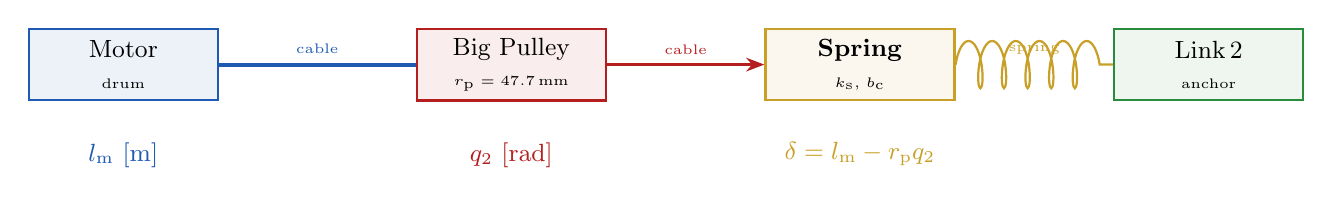
\begin{tikzpicture}[
    >=Stealth,
    block/.style={rectangle, draw=#1, thick, fill=#1!8,
                  minimum height=0.9cm, minimum width=2.4cm, align=center, font=\small},
    spring/.style={decorate, decoration={coil, aspect=0.3, segment length=3mm, amplitude=3mm}},
    cable/.style={line width=1.5pt, #1},
    arr/.style={-Stealth, thick, #1},
]
    \node[block=drakeblue] (motor)  {Motor\\{\tiny drum}};
    \node[block=darkred, right=2.5cm of motor] (pulley) {Big Pulley\\{\tiny $\rp = 47.7$\,mm}};
    \node[block=springgold, right=2.0cm of pulley] (spring) {\textbf{Spring}\\{\tiny $\ks$, $\bc$}};
    \node[block=drakegreen, right=2.0cm of spring] (link2)  {Link\,2\\{\tiny anchor}};

    \draw[cable=drakeblue] (motor.east) -- (pulley.west)
        node[midway, above, font=\tiny] {cable};
    \draw[arr=darkred] (pulley.east) -- (spring.west)
        node[midway, above, font=\tiny] {cable};
    \draw[spring, thick, springgold] (spring.east) -- (link2.west)
        node[midway, above, font=\tiny] {spring};

    % Labels
    \node[below=0.4cm of motor, font=\small, text=drakeblue] {$\lm$ [m]};
    \node[below=0.4cm of pulley, font=\small, text=darkred] {$q_2$ [rad]};
    \node[below=0.4cm of spring, font=\small, text=springgold] {$\delta = \lm - \rp q_2$};
\end{tikzpicture}
\end{center}
\end{archbox}

\subsection{State Variables}

The SEA model adds \textbf{one new state variable} to the system:

\begin{table}[H]
\centering
\caption{SEA state variable (joint~2 cable).}
\begin{tabular}{clcl}
\toprule
\textbf{Symbol} & \textbf{Description} & \textbf{Units} & \textbf{Drake storage} \\
\midrule
$\lm$ & Motor-side cable displacement (paid out by drum) & m & Discrete state \\
\bottomrule
\end{tabular}
\end{table}

The spring extension is a \emph{derived} quantity:
\begin{equation}
\boxed{\delta = \lm - \rp \, q_2}
\label{eq:delta}
\end{equation}
where $\rp$ is the big pulley radius and $q_2$ is the joint angle.  Positive $\delta$ means the spring is stretched (motor has paid out more cable than the joint has consumed).


\subsection{Spring--Damper Force}

The cable force is a linear spring--damper:
\begin{equation}
\boxed{F_{\mathrm{raw}} = \ks \, \delta + \bc \, \dot{\delta}}
\label{eq:Fraw}
\end{equation}
where:
\begin{equation}
    \dot{\delta} = \lmd - \rp \, \dot{q}_2
    \label{eq:delta_dot}
\end{equation}
Here $\lmd$ is the motor-side cable velocity, whose computation depends on the motor mode (see Section~\ref{sec:motor}).


\subsection{Antagonistic Cable Decomposition}
\label{sec:antagonistic}

The joint has \textbf{two cables} routed in opposite directions around the big pulley:

\begin{itemize}[leftmargin=2em]
    \item \textbf{Green cable} (retracting): wraps \emph{Drive $\to$ IdlerR $\to$ BigPulley $\to$ EndL}
    \item \textbf{Red cable} (extending): wraps \emph{Drive $\to$ IdlerL $\to$ BigPulley $\to$ EndR}
\end{itemize}

Cables can only \emph{pull} (tension $T \geq 0$).  The net cable force $F_{\mathrm{raw}}$ is decomposed:

\begin{equation}
\boxed{
    T_{\mathrm{green}} = \max(F_{\mathrm{raw}},\; 0), \qquad
    T_{\mathrm{red}} = \max(-F_{\mathrm{raw}},\; 0)
}
\label{eq:tensions}
\end{equation}

The \textbf{net signed cable force} applied to the joint is:
\begin{equation}
    F_{\mathrm{cable}} = T_{\mathrm{green}} - T_{\mathrm{red}} = F_{\mathrm{raw}}
\label{eq:Fnet}
\end{equation}

\begin{warnbox}
\textbf{Antagonistic means bidirectional.}  Unlike a single-cable system (which can only pull), the two-cable antagonistic arrangement allows the cable drive to produce \emph{both positive and negative} joint torque.  When $F_{\mathrm{raw}} > 0$ the green cable is taut and the red is slack; when $F_{\mathrm{raw}} < 0$ the red cable is taut and the green is slack.  Only one cable carries load at any instant (no pre-tension model).
\end{warnbox}


\subsection{Joint Torque}

The cable force maps to joint-2 torque through the pulley radius:
\begin{equation}
\boxed{\tau_2 = \rp \cdot F_{\mathrm{cable}}}
\label{eq:tau2}
\end{equation}

Joint~1 receives its torque directly from the CT controller (rigid direct-drive):
\begin{equation}
    \tau_1 = \tau_{1,\mathrm{des}}
\label{eq:tau1}
\end{equation}


% ============================================================================
\section{Motor Model}
\label{sec:motor}
% ============================================================================

The motor model is \textbf{pluggable}: two modes are supported, selectable at runtime via \texttt{--sea-mode}.  Both share the same cable spring--damper physics; only the motor dynamics differ.

\subsection{Torque Mode (Default --- 2nd-Order Rotor Dynamics)}
\label{sec:torque_mode}

In torque mode the motor runs in MIT torque/impedance mode (the default for quasi-direct-drive actuators like CubeMars AK60-6).  The rotor is modelled as an inertia $\Jm$ with viscous damping $b_{\mathrm{m}}$, driven by the commanded torque and loaded by the spring reaction through the gearbox:

\begin{equation}
\boxed{\Jm \, \ddot{\thetam} = \frac{\tau_{2,\mathrm{des}}}{N} - b_{\mathrm{m}} \, \dot{\thetam} - \frac{\rp \cdot F}{N}}
\label{eq:torque_mode}
\end{equation}

where $\thetam$ is the motor-side angle, $N$ is the gear ratio, and $F$ is the cable spring force in Newtons.

\textbf{Spring extension in linear coordinates:}
\begin{equation}
    \delta = \rp \!\left(\frac{\thetam}{N} - q_2\right), \qquad
    \dot{\delta} = \rp \!\left(\frac{\dot{\thetam}}{N} - \dot{q}_2\right)
\label{eq:delta_torque}
\end{equation}

\textbf{Cable force:}
\begin{equation}
    F = \ks \, \delta + \bc \, \dot{\delta}
\label{eq:F_torque}
\end{equation}

\textbf{Motor-side resonance frequency} (effective torsional spring at the rotor):
\begin{equation}
    \omega_n = \sqrt{\frac{\rp^2 \, \ks}{N^2 \, \Jm}}
\label{eq:omega_n}
\end{equation}

For AK60-6 with $\ks = 300$\,N/m, $\rp = 47.75$\,mm, $N = 6$: $\omega_n \approx 24$\,rad/s (4\,Hz).

\textbf{Discrete integration} (semi-implicit Euler, velocity first):
\begin{align}
    \dot{\thetam}[k{+}1] &= \dot{\thetam}[k] + \Delta t \cdot \ddot{\thetam}[k] \\
    \thetam[k{+}1] &= \thetam[k] + \Delta t \cdot \dot{\thetam}[k{+}1]
\label{eq:torque_discrete}
\end{align}

State: $[\thetam, \dot{\thetam}]$ (2 scalars, motor-side).

\begin{codemath}
The motor equation derives from Newton's second law on the rotor:
\[
    \underbrace{\Jm \, \ddot{\thetam}}_{\text{rotor inertia}} =
    \underbrace{\frac{\tau_{2,\mathrm{des}}}{N}}_{\substack{\text{motor-side}\\\text{command}}} -
    \underbrace{b_{\mathrm{m}} \, \dot{\thetam}}_{\substack{\text{viscous}\\\text{friction}}} -
    \underbrace{\frac{\rp \cdot F}{N}}_{\substack{\text{spring load}\\\text{reflected to motor}}}
\]
The spring load is computed in the \emph{linear} domain ($\delta$ in metres) to keep $\ks$ in N/m consistent across modes.
\end{codemath}


\subsection{Position Mode (Legacy --- 1st-Order Servo)}
\label{sec:position_mode}

When the motor runs a factory position controller (CAN position commands), it is modelled as a \textbf{first-order low-pass filter}:

\begin{equation}
\boxed{\lmd = \wb \, (\lm^{\mathrm{des}} - \lm)}
\label{eq:motor_servo}
\end{equation}

where $\wb$ is the position-servo bandwidth.  Discretized via forward Euler:
\begin{equation}
    \lm[k+1] = \lm[k] + \Delta t \cdot \wb \, (\lm^{\mathrm{des}}[k] - \lm[k])
\label{eq:motor_discrete}
\end{equation}

The desired motor cable position is computed by \textbf{steady-state spring inversion}:
\begin{equation}
\boxed{\lm^{\mathrm{des}} = \rp \, q_2 + \frac{\tau_{2,\mathrm{des}}}{\ks \, \rp}}
\label{eq:lm_des}
\end{equation}

State: $[\lm]$ (1 scalar, cable displacement in metres).

\begin{warnbox}
\textbf{Position-servo bandwidth is $\wb = 1/\tau_m$, NOT the no-load joint speed.}

The mechanical time constant $\tau_m = 2.5$\,ms gives an open-loop upper bound of $\wb = 1/\tau_m \approx 400$\,rad/s.  However, the closed-loop position-servo bandwidth is 2--5$\times$ lower (depends on the motor's internal PID tuning, which CubeMars does not publish).  The default is a conservative $\wb = 100$\,rad/s.

The no-load joint speed ($\omega_{\mathrm{NL,joint}} = 11.17$\,rad/s) limits \emph{maximum cable velocity}, not servo bandwidth.  These are different quantities.
\end{warnbox}


\subsection{Effect of Parameters}

\begin{table}[H]
\centering
\caption{Parameter effects on SEA behaviour.}
\begin{tabular}{ccl}
\toprule
\textbf{Parameter} & \textbf{Range} & \textbf{Effect} \\
\midrule
$\ks$ high (5000+\,N/m) & stiff & Small $\delta_{\mathrm{ss}}$ $\to$ fast torque $\to$ near-rigid \\
$\ks$ low (20--50\,N/m)  & soft  & Large $\delta_{\mathrm{ss}}$ $\to$ slow torque $\to$ high lag \\
$\wb$ high (100+\,rad/s)  & fast motor (pos.\ mode) & Tracks $\lm^{\mathrm{des}}$ quickly $\to$ less lag \\
$\wb$ low (5--10\,rad/s)  & slow motor (pos.\ mode) & Can't keep up $\to$ more lag at high speed \\
$\bc$ high & heavy damping & Suppresses oscillation, adds velocity-dependent drag \\
$\bc$ low  & light damping & Allows spring oscillation at natural frequency \\
\bottomrule
\end{tabular}
\end{table}

The SEA introduces a \textbf{fundamental bandwidth limit}: even with perfect CT, the closed-loop cannot be faster than the cable spring natural frequency:
\begin{equation}
    \omega_{\mathrm{spring}} = \sqrt{\frac{\ks \, \rp^2}{I_2}}
\end{equation}
where $I_2$ is the reflected inertia at joint~2.


% ============================================================================
\section{CubeMars AK60-6 KV80 Motor}
\label{sec:cubemars}
% ============================================================================

The elbow (joint~2) is driven by a \textbf{CubeMars AK60-6 V3.0 KV80} quasi-direct-drive actuator, which integrates a brushless DC motor with a 6:1 planetary gearbox in a compact package.  This section explains every datasheet parameter, what it physically means, and how it affects the manipulator's motion.

\subsection{Datasheet Specifications}

\begin{table}[H]
\centering
\caption{CubeMars AK60-6 KV80 --- full specification table.  All values are \emph{joint side} (after gearbox) unless marked ``motor side.''}
\label{tab:ak60_specs}
\begin{tabular}{llrl}
\toprule
\textbf{Parameter} & \textbf{Symbol} & \textbf{Value} & \textbf{Unit} \\
\midrule
\multicolumn{4}{l}{\textit{Mechanical}} \\
Gear ratio                      & $N$                  & 6       & --- \\
Peak torque (joint)             & $\tau_{\mathrm{peak}}$ & 9.0   & Nm \\
Continuous torque (joint)       & $\tau_{\mathrm{cont}}$ & 3.0   & Nm \\
No-load speed (motor side)      & $\omega_{\mathrm{NL,motor}}$ & 640 & rpm \\
No-load speed (joint side)      & $\omega_{\mathrm{NL,joint}}$ & 11.17 & rad/s \\
Rated speed (motor / joint)     &                              & 400 / 66.7 & rpm \\
Rotor inertia (motor side)      & $I_{\mathrm{r,motor}}$       & 3.3191$\times 10^{-5}$  & kg$\cdot$m$^2$ \\
Reflected inertia (joint side)  & $I_{\mathrm{r,joint}}$       & 1.195$\times 10^{-3}$  & kg$\cdot$m$^2$ \\
Viscous damping (joint)         & $b_{\mathrm{v}}$             & 0.12  & Nm$\cdot$s/rad \\
Back-drive torque               & $\tau_{\mathrm{bd}}$         & 0.2   & Nm \\
Mass                            & $m_{\mathrm{motor}}$         & 0.460 & kg \\
\midrule
\multicolumn{4}{l}{\textit{Electrical}} \\
Torque constant (motor side)    & $K_T$                & 0.11937 & Nm/A \\
Velocity constant               & $K_V$                & 80      & rpm/V \\
Rated voltage                   & $V_{\mathrm{bus}}$   & 24/48   & V \\
Rated current                   & $I_{\mathrm{rated}}$ & 4.0     & A DC \\
Peak current                    & $I_{\mathrm{peak}}$  & 11.2    & A DC \\
Pole pairs                      & $p$                  & 14      & --- \\
Phase resistance                & $R$                  & 0.595   & $\Omega$ \\
Phase inductance                & $L$                  & 675     & $\mu$H \\
Motor constant                  & $K_m$                & 0.1541  & Nm/$\sqrt{\text{W}}$ \\
Mechanical time constant        & $\tau_m$             & 2.5     & ms \\
Electrical time constant        & $\tau_e = L/R$       & 1.13    & ms \\
\bottomrule
\end{tabular}
\end{table}


\subsection{What Each Parameter Means (Plain Language)}

\begin{description}[leftmargin=2em, style=nextline, font=\bfseries\sffamily\color{seaorange}]

\item[Gear ratio ($N = 6$)]
The motor shaft turns 6 times for every single turn of the joint.  This multiplies torque by 6 but divides speed by 6.  A lower gear ratio makes the joint feel ``lighter'' and more backdrivable; a higher ratio provides more torque but adds friction and inertia.

\textit{Effect on manipulator:}  With $N=6$, the motor can push with up to 9\,Nm at the joint, which is enough for a small planar arm.  If we needed more force (e.g., lifting heavy objects), we would pick a higher gear ratio, but the arm would move slower.

\item[Peak torque ($\tau_{\mathrm{peak}} = 9.0$\,Nm)]
The \emph{maximum instantaneous} torque the motor can exert at the joint.  This is only available for short bursts (milliseconds to a few seconds) before the motor overheats.

\textit{Effect on manipulator:}  Sets the hard limit on how quickly the arm can accelerate or decelerate.  The CT controller clips torque commands to $\pm\tau_{\mathrm{peak}}$.  If the trajectory demands more torque than 9\,Nm, the arm will track poorly.

\item[Continuous torque ($\tau_{\mathrm{cont}} = 3.0$\,Nm)]
The torque the motor can sustain \emph{indefinitely} without overheating.  Think of peak torque as a sprint and continuous torque as a marathon pace.

\textit{Effect on manipulator:}  During steady-state trajectory tracking (constant speed on a rectangle), the required torque must stay below 3\,Nm or the motor will thermally shut down over time.  Gravity compensation for the arm typically requires 1--2\,Nm, well within this limit.

\item[No-load joint speed ($\omega_{\mathrm{NL,joint}} = 11.17$\,rad/s $\approx$ 107\,rpm)]
The fastest the joint can spin when there is zero torque load.  Derived from the motor's 640\,rpm no-load speed divided by the gear ratio:
\begin{equation}
    \omega_{\mathrm{NL,joint}} = \frac{640 \;\text{rpm}}{6} \times \frac{2\pi}{60} = 11.17 \;\text{rad/s}
\end{equation}

\textit{Effect on manipulator:}  Limits how fast the end-effector can sweep.  This is a \emph{velocity} limit, not a servo bandwidth.  In simulation, the motor dynamics mode determines how this is used: torque mode derives motor acceleration from rotor inertia; position mode uses $\wb = 1/\tau_m$ as the servo bandwidth (not $\omega_{\mathrm{NL,joint}}$).

\item[Reflected rotor inertia ($I_{\mathrm{r,joint}} = 1.20 \times 10^{-3}$\,kg$\cdot$m$^2$)]
How much the spinning motor rotor ``feels like'' at the joint, amplified by the square of the gear ratio:
\begin{equation}
    I_{\mathrm{r,joint}} = N^2 \cdot I_{\mathrm{r,motor}} = 36 \times 3.3191 \times 10^{-5} = 1.195 \times 10^{-3} \;\text{kg$\cdot$m$^2$}
\end{equation}

\textit{Effect on manipulator:}  Adds to the link-2 inertia that the CT controller must cancel.  For our small arm (link-2 inertia $\approx 10^{-3}$\,kg$\cdot$m$^2$), the reflected inertia is \emph{larger} than the link itself, so the arm feels noticeably heavier than its mass alone would suggest.

\item[Viscous damping ($b_{\mathrm{v}} = 0.12$\,Nm$\cdot$s/rad)]
A friction torque proportional to joint speed: $\tau_{\mathrm{friction}} = b_{\mathrm{v}} \cdot \dot{q}_2$.  Comes from the gearbox, bearings, and back-EMF effects.

\textit{Effect on manipulator:}  Acts as a natural velocity damper.  At the typical trajectory speed of $\dot{q}_2 \approx 1$\,rad/s, this contributes only 0.12\,Nm of drag---small compared to the continuous torque limit, so it does not significantly limit motion.

\item[Back-drive torque ($\tau_{\mathrm{bd}} = 0.2$\,Nm)]
The minimum external torque needed to push the joint when the motor is off.  Represents static friction (Coulomb friction + cogging torque).

\textit{Effect on manipulator:}  A low back-drive torque (0.2\,Nm for this motor) means the arm is \textbf{highly backdrivable}---you can easily push it with your finger.  This is desirable for safe human-robot interaction and for force sensing without dedicated sensors.  In simulation, this parameter is captured by Drake's joint damping.

\item[Torque constant ($K_T = 0.11937$\,Nm/A)]
Maps electric current (amps) to motor-shaft torque.  Higher $K_T$ means more torque per amp, but lower speed per volt.

\textit{Effect on manipulator:}  Determines how much current the motor driver must supply.  At peak joint torque: $I_{\mathrm{peak}} = \tau_{\mathrm{peak}} / (N \cdot K_T) = 9 / (6 \times 0.11937) = 12.6$\,A.  The datasheet reports 11.2\,A peak (driver-limited), so the motor cannot quite reach full 9\,Nm in practice.

\item[Rated voltage ($V_{\mathrm{bus}} = 48$\,V)]
The supply voltage that determines maximum speed.  Higher voltage $\to$ higher no-load speed.

\textit{Effect on manipulator:}  At 48\,V, the motor achieves its rated 640\,rpm.  Running at 24\,V would halve the max speed but keep torque the same (current-limited).  In simulation, voltage is not modelled; motor bandwidth emerges from rotor inertia (torque mode) or position-servo bandwidth $\wb$ (position mode).

\end{description}


\subsection{Mapping Motor Specs to Simulation Parameters}
\label{sec:motor_mapping}

The simulation does \emph{not} model the full electrical dynamics (current loop, PWM, etc.).  Instead, the motor's complex electromechanical behaviour is captured by a few parameters whose mapping depends on the motor mode:

\begin{table}[H]
\centering
\caption{Datasheet $\to$ simulation parameter mapping.}
\label{tab:motor_mapping}
\begin{tabular}{llll}
\toprule
\textbf{Sim.\ Parameter} & \textbf{Derived From} & \textbf{Formula / Value} & \textbf{Mode} \\
\midrule
$\Jm$ [kg$\cdot$m$^2$] — rotor inertia & Datasheet (motor side) & $3.3191\times10^{-5}$ & Torque \\
$b_{\mathrm{m}}$ [Nm$\cdot$s/rad] — motor damping & $b_{\mathrm{v,joint}} / N^2$ & $0.12 / 36 = 3.33\times10^{-3}$ & Torque \\
$N$ — gear ratio & Gearbox spec & $6$ & Both \\
$\wb$ [rad/s] — servo bandwidth & $1 / \tau_m$ (open-loop) & $1 / 0.0025 = 400$ (default: 100) & Position \\
$\tau_{\max}$ [Nm] — torque clip & Peak torque & $\tau_{\mathrm{peak}} = 9.0$ & Both \\
Joint damping [Nm$\cdot$s/rad] & Viscous damping & $b_{\mathrm{v}} = 0.12$ & Both \\
\bottomrule
\end{tabular}
\end{table}

\begin{warnbox}
\textbf{Position-mode bandwidth: $\wb = 1/\tau_m$, not $\omega_{\mathrm{NL,joint}}$.}

The mechanical time constant $\tau_m = \Jm \cdot R / K_T^2 = 2.5$\,ms gives an open-loop upper bound $\wb = 400$\,rad/s.  The no-load joint speed $\omega_{\mathrm{NL,joint}} = 11.17$\,rad/s is a \emph{velocity} limit, not a bandwidth.  CubeMars does not publish closed-loop position-servo bandwidth, so the CLI default is a conservative 100\,rad/s ($\approx 4\times$ below the open-loop limit).

In \textbf{torque mode} (default), there is no explicit $\wb$; motor bandwidth emerges from the rotor inertia, damping, and spring dynamics (see Section~\ref{sec:torque_mode}).
\end{warnbox}

\begin{archbox}{Motor Torque--Speed Tradeoff}
\begin{center}
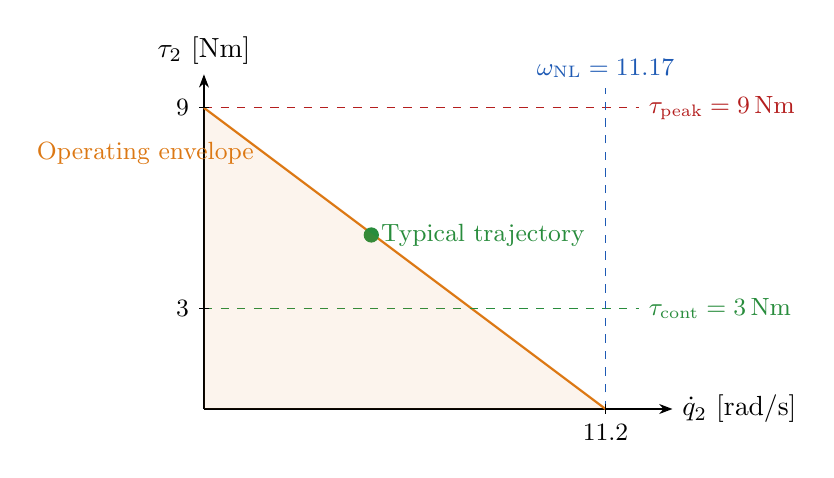
\begin{tikzpicture}[>=Stealth, scale=0.85]
    % Axes
    \draw[->] (0,0) -- (7,0) node[right] {$\dot{q}_2$ [rad/s]};
    \draw[->] (0,0) -- (0,5) node[above] {$\tau_2$ [Nm]};

    % Torque-speed line
    \draw[thick, seaorange] (0,4.5) -- (6,0)
        node[pos=0.15, left, font=\small] {Operating envelope};

    % Peak torque
    \draw[dashed, darkred] (0,4.5) -- (6.5,4.5)
        node[right, font=\small, text=darkred] {$\tau_{\mathrm{peak}} = 9$\,Nm};

    % Continuous torque
    \draw[dashed, drakegreen] (0,1.5) -- (6.5,1.5)
        node[right, font=\small, text=drakegreen] {$\tau_{\mathrm{cont}} = 3$\,Nm};

    % No-load speed
    \draw[dashed, drakeblue] (6,0) -- (6,4.8)
        node[above, font=\small, text=drakeblue] {$\omega_{\mathrm{NL}} = 11.17$};

    % Typical operating point
    \filldraw[drakegreen] (2.5,2.6) circle (3pt)
        node[right, font=\small] {Typical trajectory};

    % Shaded region
    \fill[seaorange, opacity=0.08] (0,0) -- (0,4.5) -- (6,0) -- cycle;

    % Axis ticks
    \foreach \y/\label in {1.5/3, 4.5/9}
        \draw (0.08,\y) -- (-0.08,\y) node[left, font=\small] {\label};
    \draw (6,0.08) -- (6,-0.08) node[below, font=\small] {11.2};
\end{tikzpicture}
\end{center}
The motor can produce high torque at low speed or high speed at low torque, but not both simultaneously.  Trajectory tracking typically operates in the green region.
\end{archbox}


% ============================================================================
\section{SEA Equations: Derivation from First Principles}
\label{sec:sea_derivation}
% ============================================================================

This section derives the complete SEA cable model step by step, starting from the physical setup and ending with the equations implemented in code.

\subsection{Step 1: Define the Spring Extension}

Consider the cable path: the motor drum pays out a cable of length $\lm$ [m].  This cable wraps around the big pulley (radius $\rp$) and connects to a spring anchored on link~2.  The amount of cable ``consumed'' by the joint rotation is $\rp \cdot q_2$.

The \textbf{spring extension} is simply the difference between what the motor has paid out and what the joint has consumed:
\begin{equation}
\boxed{\delta = \lm - \rp \, q_2}
\end{equation}

\begin{itemize}[leftmargin=2em]
    \item $\delta > 0$: motor has paid out more cable than needed $\to$ spring is stretched $\to$ it pulls the joint forward
    \item $\delta < 0$: joint has rotated further than the motor $\to$ spring is compressed $\to$ it pushes back
    \item $\delta = 0$: spring at rest, no force
\end{itemize}


\subsection{Step 2: Spring--Damper Force}

The cable element between the pulley and link~2 behaves as a \textbf{parallel spring--damper}:
\begin{equation}
\boxed{F_{\mathrm{raw}} = \underbrace{\ks \, \delta}_{\text{elastic}} + \underbrace{\bc \, \dot{\delta}}_{\text{viscous}}}
\end{equation}

The spring stiffness $\ks$ [N/m] is the cable/belt elasticity (or an explicit compliance element).  The damping $\bc$ [N$\cdot$s/m] models internal friction in the cable.

The spring extension rate $\dot{\delta}$ is:
\begin{equation}
    \dot{\delta} = \lmd - \rp \, \dot{q}_2
\end{equation}
That is, the spring stretches when the motor pulls cable in faster than the joint rotates, and compresses when the joint outruns the motor.


\subsection{Step 3: Motor Dynamics}

The motor does not jump instantly to the desired state.  The dynamics depend on the selected mode:

\medskip
\textbf{Torque mode} (default).  The rotor is an inertia loaded by the spring:
\begin{equation}
\boxed{\Jm \, \ddot{\thetam} = \frac{\tau_{2,\mathrm{des}}}{N} - b_{\mathrm{m}} \, \dot{\thetam} - \frac{\rp \cdot F}{N}}
\end{equation}

The motor's bandwidth is \emph{not} a single number---it emerges from the coupled motor--spring dynamics.  The motor-side resonance is $\omega_n = \sqrt{\rp^2 \ks / (N^2 \Jm)}$, which for AK60-6 and $\ks = 300$\,N/m is $\approx 24$\,rad/s.

\medskip
\textbf{Position mode} (legacy).  The motor tracks a target cable position as a first-order lag:
\begin{equation}
\boxed{\lmd = \wb \, (\lm^{\mathrm{des}} - \lm)}
\end{equation}

\textbf{Where does $\wb$ come from?}  It is the position-servo bandwidth, derived from the mechanical time constant: $\wb = 1/\tau_m \approx 400$\,rad/s (open-loop upper bound for AK60-6).  The CLI default is a conservative 100\,rad/s because the closed-loop bandwidth is lower (see Section~\ref{sec:motor_mapping}).

In discrete time (simulation timestep $\Delta t = 2$\,ms):
\begin{equation}
    \lm[k+1] = \lm[k] + \Delta t \cdot \wb \cdot (\lm^{\mathrm{des}}[k] - \lm[k])
\end{equation}

\begin{codemath}
\textbf{Transfer function} of the position-mode motor servo (Laplace domain):
\[
    \frac{L_m(s)}{L_m^{\mathrm{des}}(s)} = \frac{\wb}{s + \wb}
\]
This is a first-order low-pass with cutoff frequency $\wb$.  At frequencies above $\wb$, the motor cannot track the commanded cable position---this is the fundamental source of lag in position-mode SEA.
\end{codemath}


\subsection{Step 4: Steady-State Spring Inversion}

The controller needs to tell the motor \emph{where} to position the cable so that the spring produces the desired torque.  At steady state (motor has reached its target, spring extension rate is zero):
\begin{align}
    \tau_{2,\mathrm{des}} &= \rp \cdot F_{\mathrm{cable}} = \rp \cdot \ks \cdot \delta_{\mathrm{ss}} \\
    \Rightarrow\quad \delta_{\mathrm{ss}} &= \frac{\tau_{2,\mathrm{des}}}{\ks \, \rp} \\
    \Rightarrow\quad \lm^{\mathrm{des}} &= \underbrace{\rp \, q_2}_{\text{joint position}} + \underbrace{\frac{\tau_{2,\mathrm{des}}}{\ks \, \rp}}_{\text{spring stretch needed}}
\end{align}

\begin{equation}
\boxed{\lm^{\mathrm{des}} = \rp \, q_2 + \frac{\tau_{2,\mathrm{des}}}{\ks \, \rp}}
\end{equation}

\textbf{Plain language}: ``The motor must pay out enough cable to match the joint angle, \emph{plus} a little extra to stretch the spring by the amount needed to produce the desired force.''


\subsection{Step 5: From Cable Force to Joint Torque}

The cable force maps to joint torque through the pulley radius (moment arm):
\begin{equation}
\boxed{\tau_2 = \rp \cdot F_{\mathrm{cable}}}
\end{equation}

With the antagonistic cable arrangement (Section~\ref{sec:antagonistic}), the net cable force is:
\[
    F_{\mathrm{cable}} = T_{\mathrm{green}} - T_{\mathrm{red}} = F_{\mathrm{raw}}
\]
where each tension is non-negative (cables only pull).


\subsection{Step 6: Effect of Spring Stiffness on Tracking}

The effect of $\ks$ on tracking quality depends on the motor mode.  The two modes exhibit \emph{opposite} trends.

\medskip
\textbf{Torque mode (default) --- stiffer is better.}\quad
In torque mode the motor bandwidth is \emph{not} fixed; it emerges from the coupled rotor--spring dynamics.  The motor-side resonance frequency scales with $\sqrt{\ks}$:
\begin{equation}
    \omega_n = \sqrt{\frac{\rp^2 \, \ks}{N^2 \, \Jm}}
    \qquad \Longrightarrow \qquad
    \omega_n \propto \sqrt{\ks}
\end{equation}
Increasing $\ks$ raises $\omega_n$, making the motor--spring system respond \emph{faster}.  Simultaneously, the steady-state spring deflection needed to produce a given torque \emph{decreases}:
\begin{equation}
    \delta_{\mathrm{ss}} = \frac{\tau_{2,\mathrm{des}}}{\ks \, \rp}
    \quad \xrightarrow{\;\ks \uparrow\;}
    \quad 0
\end{equation}
Both effects work in the same direction: \textbf{stiffer springs yield better tracking in torque mode}.  In the limit $\ks \to \infty$, the SEA degenerates to a rigid tendon.  This is confirmed by simulation (Section~\ref{sec:results}): $\ks = 30{,}000$\,N/m achieves near-rigid performance ($<5$\,mm EE error, $\tau$ RMS error $0.004$\,Nm), while $\ks = 30$\,N/m produces $\sim$25\,mm EE error with 10$\times$ worse torque tracking.

\medskip
\textbf{Position mode (legacy) --- stiffer is worse.}\quad
In position mode the motor servo has a \emph{fixed} bandwidth $\wb$, so the motor position error $\varepsilon$ is approximately constant regardless of $\ks$.  The resulting \textbf{torque error} scales linearly with stiffness:
\begin{equation}
\boxed{\Delta\tau_{\mathrm{pos}} \;\approx\; \rp \cdot \ks \cdot \varepsilon}
\end{equation}

With a soft spring ($\ks = 30$\,N/m): $\Delta\tau \approx 0.048 \times 30 \times \varepsilon \approx 1.4\,\varepsilon$\,Nm.

With a stiff spring ($\ks = 3000$\,N/m): $\Delta\tau \approx 0.048 \times 3000 \times \varepsilon \approx 144\,\varepsilon$\,Nm.

The stiff spring amplifies the same small motor position lag into a \emph{much larger} torque error.  The fix: increase $\wb$ proportionally to $\ks$.

\begin{resultbox}
\textbf{Torque mode (default):}\quad Stiffer spring $\;\to\;$ higher motor--spring resonance $\omega_n \propto \sqrt{\ks}$ $\;\to\;$ \textbf{better tracking}.  No bandwidth tuning required---the 2nd-order rotor dynamics adapt naturally to stiffer springs.

\medskip
\textbf{Position mode (legacy):}\quad Stiffer spring $\;\to\;$ larger torque error $\Delta\tau \propto \ks \cdot \varepsilon$ if $\wb$ is held constant.  To maintain tracking accuracy:
\[
    \frac{\ks}{\wb} = \text{const} \qquad \Longrightarrow \qquad \text{constant torque tracking error}
\]
If $\ks$ increases by $100\times$, $\wb$ should also increase by $100\times$.  Physically limited by motor hardware ($\omega_{\mathrm{b,max}} \approx 400$\,rad/s for AK60-6).
\end{resultbox}


% ============================================================================
\section{Control Architecture}
\label{sec:control}
% ============================================================================

\subsection{Two-Layer Architecture}

\begin{archbox}{SEA Control Loop}
\begin{center}
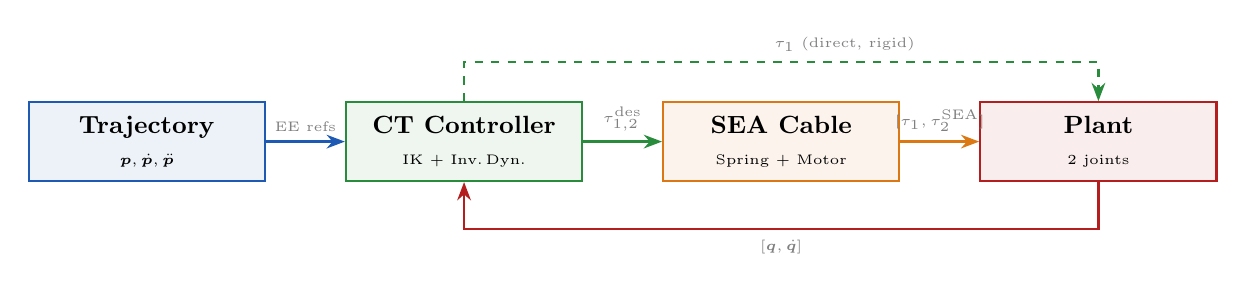
\begin{tikzpicture}[
    node distance=0.6cm and 1.2cm,
    block/.style={rectangle, draw=#1, thick, fill=#1!8,
                  minimum height=1cm, minimum width=3cm, align=center, font=\small},
    arr/.style={-Stealth, thick, #1},
    port/.style={font=\tiny, text=gray},
]
    \node[block=drakeblue] (ref) {\textbf{Trajectory}\\{\tiny $\bm{p}, \dot{\bm{p}}, \ddot{\bm{p}}$}};
    \node[block=drakegreen, right=1cm of ref] (ct) {\textbf{CT Controller}\\{\tiny IK + Inv.\,Dyn.}};
    \node[block=seaorange, right=1cm of ct] (sea) {\textbf{SEA Cable}\\{\tiny Spring + Motor}};
    \node[block=darkred, right=1cm of sea] (plant) {\textbf{Plant}\\{\tiny 2 joints}};

    \draw[arr=drakeblue] (ref) -- (ct) node[midway, above, port] {EE refs};
    \draw[arr=drakegreen] (ct) -- (sea) node[midway, above, port] {$\tau_{1,2}^{\mathrm{des}}$};
    \draw[arr=seaorange] (sea) -- (plant) node[midway, above, port] {$[\tau_1, \tau_2^{\mathrm{SEA}}]$};
    \draw[arr=darkred] (plant.south) -- ++(0,-0.6) -| (ct.south)
        node[pos=0.25, below, port] {$[\bq, \dot{\bq}]$};

    % Joint 1 shortcut
    \draw[arr=drakegreen, dashed] (ct.north) -- ++(0,0.5) -| (plant.north)
        node[pos=0.3, above, port] {$\tau_1$ (direct, rigid)};
\end{tikzpicture}
\end{center}
\end{archbox}

\subsection{Per-Timestep Algorithm}

At each simulation step ($\Delta t = 2$\,ms), the two blocks execute in sequence:

\medskip
\textbf{Block 1 --- \texttt{ComputedTorqueController}} (controller/controller.py):
\begin{enumerate}[leftmargin=2em]
    \item \textbf{Read plant state} $(q_1, q_2, \dot{q}_1, \dot{q}_2)$
    \item \textbf{Analytical 2R IK}: $\bm{p}_{\mathrm{ref}} \to (q_{1}^{\mathrm{des}}, q_{2}^{\mathrm{des}})$
    \item \textbf{Differential IK}: $\dot{\bm{p}}_{\mathrm{ref}} \xrightarrow{\bJ^{-1}} \dot{\bq}_{\mathrm{ref}}$, \quad $\ddot{\bm{p}}_{\mathrm{ref}} \xrightarrow{\bJ^{-1}} \ddot{\bq}_{\mathrm{ref}}$
    \item \textbf{PD + feedforward}: $\bm{a}_{\mathrm{des}} = \ddot{\bq}_{\mathrm{ref}} + K_p(\bq_{\mathrm{des}} - \bq) + K_d(\dot{\bq}_{\mathrm{ref}} - \dot{\bq})$
    \item \textbf{Inverse dynamics}: $\btau_{\mathrm{des}} = \bM(\bq)\,\bm{a}_{\mathrm{des}} + \bh(\bq, \dot{\bq})$
\end{enumerate}

\textbf{Block 2 --- \texttt{SEACableActuator}} (actuators/sea.py), delegating to a \texttt{MotorDynamics} subclass:

\medskip
\textit{Torque mode} (default, \texttt{TorqueMotor}):
\begin{enumerate}[leftmargin=2em, start=6]
    \item \textbf{Motor command}: $\tau_m = \tau_{2,\mathrm{des}} / N$
    \item \textbf{Cable force}: $\delta = \rp(\thetam/N - q_2)$, \quad $F = \ks\,\delta + \bc\,\dot{\delta}$
    \item \textbf{Rotor update} (semi-implicit Euler): $\ddot{\thetam} = (\tau_m - b_{\mathrm{m}}\,\dot{\thetam} - \rp F/N) / \Jm$, \quad update $[\thetam, \dot{\thetam}]$
    \item \textbf{Tension decomposition}: $T_{\mathrm{green}} = \max(F, 0)$, \quad $T_{\mathrm{red}} = \max(-F, 0)$
    \item \textbf{Apply torque}: $\tau_1 = \tau_{1,\mathrm{des}}$ (rigid), \quad $\tau_2 = \rp \cdot (T_{\mathrm{green}} - T_{\mathrm{red}})$
\end{enumerate}

\textit{Position mode} (legacy, \texttt{PositionServoMotor}):
\begin{enumerate}[leftmargin=2em, start=6]
    \item \textbf{Motor target} (steady-state inversion): $\lm^{\mathrm{des}} = \rp \, q_2 + \tau_{2,\mathrm{des}} / (\ks \, \rp)$
    \item \textbf{Motor update} (Euler step): $\lm \gets \lm + \Delta t \cdot \wb \cdot (\lm^{\mathrm{des}} - \lm)$
    \item \textbf{Spring force}: $\delta = \lm - \rp q_2$, \quad $F = \ks \delta + \bc \dot{\delta}$
    \item \textbf{Tension decomposition}: $T_{\mathrm{green}} = \max(F, 0)$, \quad $T_{\mathrm{red}} = \max(-F, 0)$
    \item \textbf{Apply torque}: $\tau_1 = \tau_{1,\mathrm{des}}$ (rigid), \quad $\tau_2 = \rp \cdot (T_{\mathrm{green}} - T_{\mathrm{red}})$
\end{enumerate}

Steps 1--5 are the standard CT pipeline (identical to the rigid-tendon controller).  Steps 6--10 are the SEA cable layer.  Because these are separate Drake \texttt{LeafSystem}s, any controller that outputs $[\tau_1, \tau_2]$ can be substituted for the CT block.


\subsection{Detailed Signal-Flow Block Diagram}
\label{sec:block_diagram}

Figure~\ref{fig:block_diagram} shows the complete signal-flow graph for the two-block architecture.

\begin{figure}[H]
\centering
\resizebox{\textwidth}{!}{%
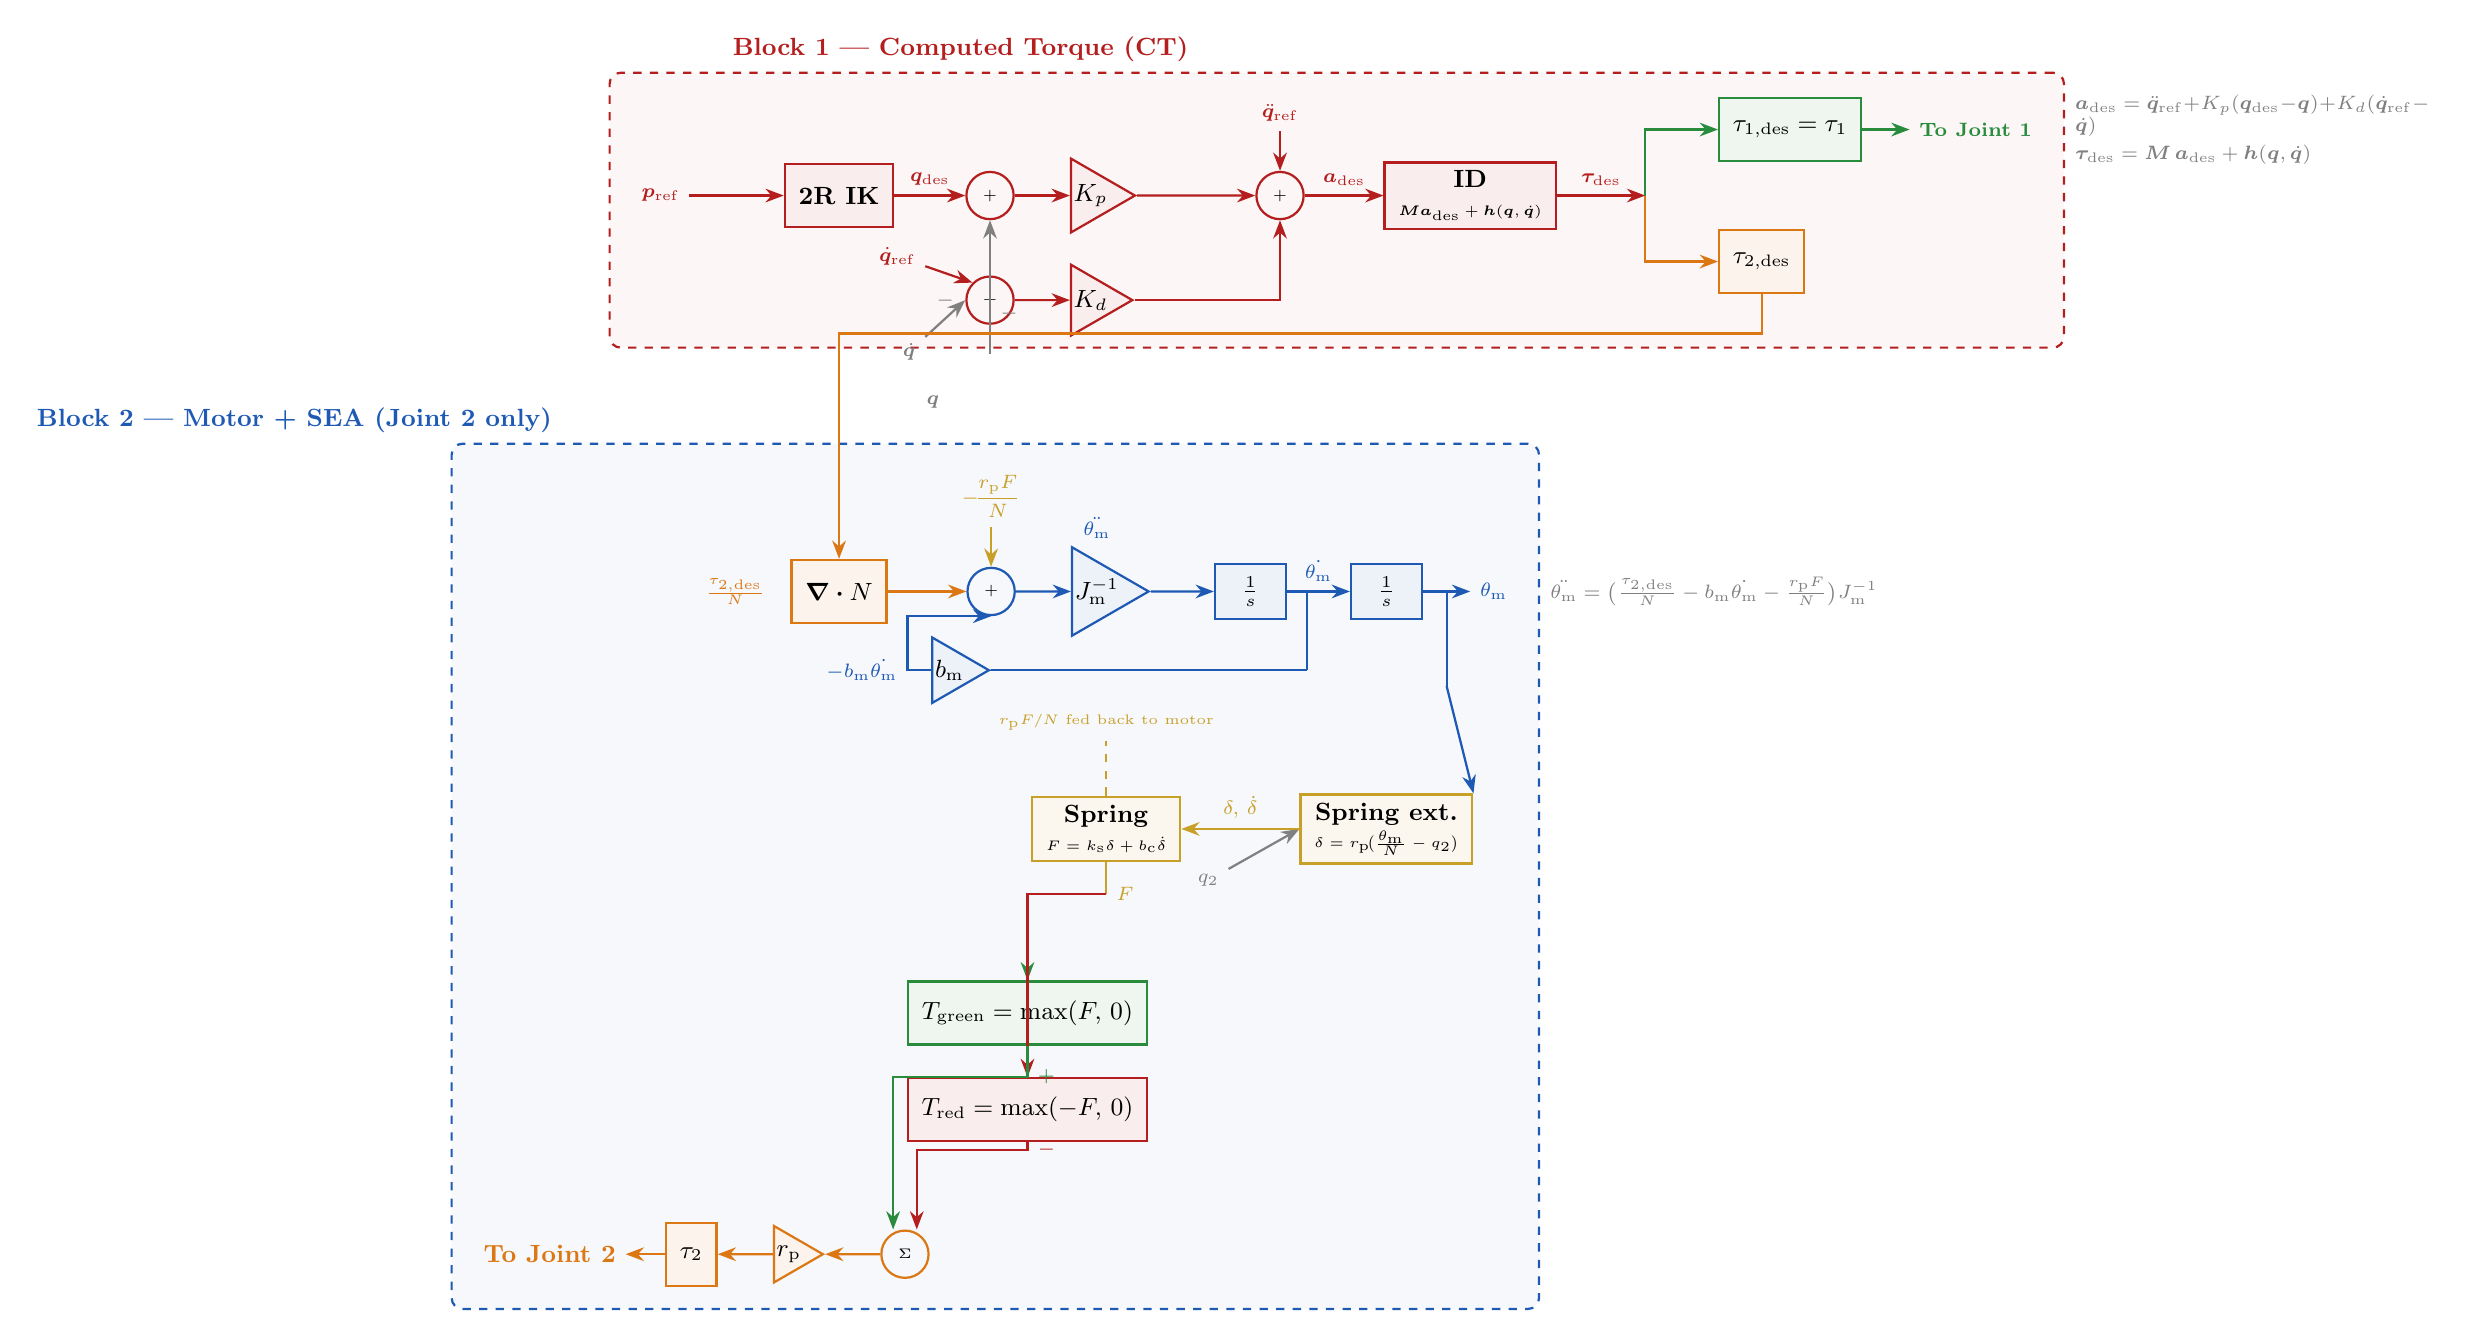
\begin{tikzpicture}[
    >=Stealth,
    % --- node styles ---
    sumnode/.style={circle, draw=#1, thick, inner sep=0pt,
                    minimum size=6mm, font=\scriptsize},
    block/.style={rectangle, draw=#1, thick, fill=#1!8,
                  minimum height=8mm, align=center, font=\small,
                  inner xsep=5pt, inner ysep=3pt},
    gain/.style={isosceles triangle, draw=#1, thick, fill=#1!8,
                 isosceles triangle apex angle=60,
                 minimum width=7mm, minimum height=5mm,
                 shape border rotate=0, font=\small, inner sep=1pt},
    integ/.style={rectangle, draw=drakeblue, thick, fill=drakeblue!8,
                  minimum height=7mm, minimum width=9mm,
                  align=center, font=\small},
    arr/.style={-Stealth, thick, #1},
    sig/.style={font=\scriptsize, text=#1},
    note/.style={font=\scriptsize\itshape, text=gray},
    % --- group boxes ---
    groupbox/.style={draw=#1, thick, dashed, rounded corners=4pt,
                     fill=#1!4, inner sep=8pt},
]

% ========================================================================
%  BLOCK 1: Computed Torque Controller (upper half)
% ========================================================================

% ── IK ──
\node[block=darkred] (ik) {\textbf{2R IK}};
\node[left=1.2cm of ik, sig=darkred] (pref) {$\bm{p}_{\mathrm{ref}}$};
\draw[arr=darkred] (pref) -- (ik);

% ── Sum node (q error) ──
\node[sumnode=darkred, right=0.9cm of ik] (qsum) {};
\draw (qsum.center) node[font=\tiny] {$+$};
\draw[arr=darkred] (ik) -- (qsum)
    node[midway, above, sig=darkred] {$\bq_{\mathrm{des}}$};

% ── Kp gain ──
\node[gain=darkred, right=0.7cm of qsum] (kp) {$K_p$};
\draw[arr=darkred] (qsum) -- (kp);

% ── Bottom path: Kd gain (velocity error) ──
\node[sumnode=darkred, below=0.7cm of qsum] (qdotsum) {};
\draw (qdotsum.center) node[font=\tiny] {$+$};
\node[gain=darkred, right=0.7cm of qdotsum] (kd) {$K_d$};
\draw[arr=darkred] (qdotsum) -- (kd);

% ── a_des sum node ──
\node[sumnode=darkred, right=1.5cm of kp] (asum) {};
\draw (asum.center) node[font=\tiny] {$+$};
\draw[arr=darkred] (kp) -- (asum);
\draw[arr=darkred] (kd.east) -| (asum);

% ── q_ref_ddot feedforward ──
\node[above=0.5cm of asum, sig=darkred] (qddref) {$\ddot{\bq}_{\mathrm{ref}}$};
\draw[arr=darkred] (qddref) -- (asum);

% ── ID block ──
\node[block=darkred, right=1.0cm of asum] (id) {\textbf{ID}\\[-1pt]{\tiny $\bM\bm{a}_{\mathrm{des}} + \bh(\bq,\dot{\bq})$}};
\draw[arr=darkred] (asum) -- (id)
    node[midway, above, sig=darkred] {$\bm{a}_{\mathrm{des}}$};

% ── τ_des output ──
\node[right=1.0cm of id] (tdes_split) {};
\draw[arr=darkred] (id) -- (tdes_split.center)
    node[midway, above, sig=darkred] {$\btau_{\mathrm{des}}$};

% ── τ_1,des = τ_1 (direct) ──
\node[block=drakegreen, above right=0.3cm and 0.8cm of tdes_split] (tau1) {$\tau_{1,\mathrm{des}} = \tau_1$};
\draw[arr=drakegreen] (tdes_split.center) |- (tau1);
\node[right=0.6cm of tau1, sig=drakegreen] (tau1out) {\textbf{To Joint 1}};
\draw[arr=drakegreen] (tau1) -- (tau1out);

% ── τ_2,des output ──
\node[block=seaorange, below right=0.3cm and 0.8cm of tdes_split] (tau2box) {$\tau_{2,\mathrm{des}}$};
\draw[arr=seaorange] (tdes_split.center) |- (tau2box);

% ── feedback arrows ──
% q feedback to qsum
\coordinate (qfb_entry) at ($(qsum.south) + (0, -1.7)$);
\node[below left=2.2cm and 0.3cm of qsum, sig=gray] (qfb_label) {$\bq$};
\draw[arr=gray] (qfb_entry) -- (qsum.south)
    node[pos=0.3, right, sig=gray] {$-$};
% qdot feedback to qdotsum
\node[below left=0.2cm and 0.6cm of qdotsum, sig=gray] (qdotfb_label) {$\dot{\bq}$};
\draw[arr=gray] (qdotfb_label) -- (qdotsum.west)
    node[pos=0.5, above, sig=gray] {$-$};
% qdot_ref from IK
\node[above left=0.1cm and 0.6cm of qdotsum, sig=darkred] (qdotref) {$\dot{\bq}_{\mathrm{ref}}$};
\draw[arr=darkred] (qdotref) -- (qdotsum.north west);

% ── Block 1 group box ──
\begin{scope}[on background layer]
    \node[groupbox=darkred,
          fit=(pref)(ik)(qsum)(qdotsum)(kp)(kd)(asum)(qddref)(id)(tau1)(tau1out)(tau2box),
          label={[font=\bfseries\small, text=darkred]above left:Block 1 --- Computed Torque (CT)}] (b1box) {};
\end{scope}

% ========================================================================
%  BLOCK 2: Motor + SEA (lower half)
% ========================================================================

% Position Block 2 below Block 1
\coordinate (b2origin) at ($(ik.south) + (0, -4.2)$);

% ── τ_2,des / N ──
\node[block=seaorange, anchor=north] at (b2origin) (divN) {$\div N$};
\draw[arr=seaorange] (tau2box.south) -- ++(0,-0.5) -| (divN.north);
\node[left=0.2cm of divN, sig=seaorange] (tauN_lab) {$\frac{\tau_{2,\mathrm{des}}}{N}$};

% ── Motor dynamics sum node ──
\node[sumnode=drakeblue, right=1.0cm of divN] (msum) {};
\draw (msum.center) node[font=\tiny] {$+$};
\draw[arr=seaorange] (divN) -- (msum);

% ── 1/Jm gain ──
\node[gain=drakeblue, right=0.7cm of msum] (invJm) {$\Jm^{-1}$};
\draw[arr=drakeblue] (msum) -- (invJm);

% ── θ̈_m label ──
\node[above=0.15cm of invJm, sig=drakeblue] (thetaddm_lab) {$\ddot{\thetam}$};

% ── Integrator 1: θ̈_m → θ̇_m ──
\node[integ, right=0.8cm of invJm] (int1) {$\frac{1}{s}$};
\draw[arr=drakeblue] (invJm) -- (int1);

% ── Integrator 2: θ̇_m → θ_m ──
\node[integ, right=0.8cm of int1] (int2) {$\frac{1}{s}$};
\draw[arr=drakeblue] (int1) -- (int2)
    node[midway, above, sig=drakeblue] {$\dot{\thetam}$};

% ── θ_m output ──
\node[right=0.6cm of int2, sig=drakeblue] (thetam_out) {$\thetam$};
\draw[arr=drakeblue] (int2) -- (thetam_out);

% ── b_m feedback loop ──
\coordinate (bm_fb_right) at ($(int1.east) + (0.25, 0)$);
\coordinate (bm_fb_down) at ($(bm_fb_right) + (0, -1.0)$);
\node[gain=drakeblue, anchor=east] at ($(msum.center) + (0, -1.0)$) (bm) {$b_{\mathrm{m}}$};
\draw[drakeblue, thick] (bm_fb_right) -- (bm_fb_down);
\draw[drakeblue, thick] (bm_fb_down) -| (bm.east);
\draw[arr=drakeblue] (bm.west) -- ++(- 0.3, 0) |- (msum.south)
    node[pos=0.0, left, sig=drakeblue] {$-b_{\mathrm{m}} \dot{\thetam}$};

% ── r_pF/N feedback into motor sum ──
\coordinate (rpFN_entry) at ($(msum.north) + (0, 0.5)$);
\node[above=0.5cm of msum, sig=springgold] (rpFN_lab) {$-\!\dfrac{\rp F}{N}$};
\draw[arr=springgold] (rpFN_lab) -- (msum.north);

% ── Spring computation (below θ_m path) ──
% δ computation
\node[block=springgold, below=2.2cm of int2] (delta_block)
    {\textbf{Spring ext.}\\[-1pt]{\tiny $\delta = \rp\!\bigl(\frac{\thetam}{N} - q_2\bigr)$}};

% Route θ_m down to δ block
\coordinate (thetam_down) at ($(int2.east) + (0.3, 0)$);
\draw[drakeblue, thick] (thetam_down) -- ++(0, -1.2);
\draw[arr=drakeblue] ($(thetam_down) + (0, -1.2)$) -- (delta_block.north east);

% q₂ input to δ block
\node[below left=0.0cm and 0.9cm of delta_block, sig=gray] (q2in) {$q_2$};
\draw[arr=gray] (q2in) -- (delta_block.west);

% ── Spring force ──
\node[block=springgold, left=1.5cm of delta_block] (spring_f)
    {\textbf{Spring}\\[-1pt]{\tiny $F = \ks\delta + \bc\dot{\delta}$}};
\draw[arr=springgold] (delta_block) -- (spring_f)
    node[midway, above, sig=springgold] {$\delta,\,\dot{\delta}$};

% ── Unilateral split ──
\node[block=drakegreen, below=1.5cm of spring_f, xshift=-1.0cm] (tgreen)
    {$T_{\mathrm{green}} = \max(F,\,0)$};
\node[block=darkred, below=0.4cm of tgreen] (tred)
    {$T_{\mathrm{red}} = \max(-F,\,0)$};

\coordinate (F_split) at ($(spring_f.south) + (0, -0.4)$);
\draw[springgold, thick] (spring_f.south) -- (F_split)
    node[right, sig=springgold] {$F$};
\draw[arr=drakegreen] (F_split) -| (tgreen.north);
\draw[arr=darkred] (F_split) -| (tred.north);

% ── τ₂ = r_p(T_green - T_red) ──
\node[sumnode=seaorange, below left=1.2cm and -0.2cm of tred] (tausum) {};
\draw (tausum.center) node[font=\tiny] {$\Sigma$};
\draw[arr=drakegreen] (tgreen.south) -- ++(0,-0.4) -| ($(tausum.north) + (-0.15, 0)$)
    node[pos=0.0, right, sig=drakegreen] {$+$};
\draw[arr=darkred] (tred.south) -- ++(0,-0.1) -| ($(tausum.north) + (0.15, 0)$)
    node[pos=0.0, right, sig=darkred] {$-$};

\node[gain=seaorange, left=0.7cm of tausum] (rp_gain) {$\rp$};
\draw[arr=seaorange] (tausum) -- (rp_gain);

% ── τ₂ output ──
\node[block=seaorange, left=0.7cm of rp_gain] (tau2out)
    {$\tau_2$};
\draw[arr=seaorange] (rp_gain) -- (tau2out);
\node[left=0.5cm of tau2out, sig=seaorange, font=\small\bfseries] (jt2out) {\textbf{To Joint 2}};
\draw[arr=seaorange] (tau2out) -- (jt2out);

% ── r_pF/N feedback path from spring to motor sum ──
\draw[springgold, thick, dashed] (spring_f.north) -- ++(0, 0.7)
    node[above, sig=springgold] {\tiny $\rp F / N$ fed back to motor};

% ── Block 2 group box ──
\begin{scope}[on background layer]
    \node[groupbox=drakeblue,
          fit=(divN)(msum)(invJm)(int1)(int2)(thetam_out)(bm)(delta_block)(spring_f)(tgreen)(tred)(tausum)(rp_gain)(tau2out)(jt2out)(q2in)(rpFN_lab)(tauN_lab),
          label={[font=\bfseries\small, text=drakeblue]above left:Block 2 --- Motor + SEA (Joint 2 only)}] (b2box) {};
\end{scope}

% ========================================================================
%  ANNOTATION: key equations
% ========================================================================
\node[note, right=0.3cm of tau1out, text width=4.5cm] (eq_ct)
    {$\bm{a}_{\mathrm{des}} = \ddot{\bq}_{\mathrm{ref}} + K_p(\bq_{\mathrm{des}} - \bq) + K_d(\dot{\bq}_{\mathrm{ref}} - \dot{\bq})$\\[2pt]
     $\btau_{\mathrm{des}} = \bM\,\bm{a}_{\mathrm{des}} + \bh(\bq,\dot{\bq})$};

\node[note, right=0.3cm of thetam_out, text width=4.5cm] (eq_motor)
    {$\ddot{\thetam} = \bigl(\frac{\tau_{2,\mathrm{des}}}{N} - b_{\mathrm{m}}\dot{\thetam} - \frac{\rp F}{N}\bigr) \Jm^{-1}$};

\end{tikzpicture}
}% end resizebox
\caption{Detailed signal-flow block diagram.
    \textbf{Block~1} (upper, red): Computed-Torque controller---2R inverse kinematics, PD error with feedforward, inverse dynamics.
    $\tau_1$ goes directly to joint~1 (rigid).
    $\tau_{2,\mathrm{des}}$ enters \textbf{Block~2} (lower, blue): motor rotor dynamics with viscous damping $b_{\mathrm{m}}$, cable spring--damper, unilateral tension split, and pulley radius mapping to joint torque $\tau_2$.}
\label{fig:block_diagram}
\end{figure}


% ============================================================================
\section{Exosuit Co-Contraction Stiffness}
\label{sec:exosuit}
% ============================================================================

The exosuit adds a \textbf{parallel stiffness layer} on joint~2 using two
antagonistic cable--spring--motor chains (right and left) routed around a
shared centred elbow pulley (Method~B, see cable documentation).
It does \emph{not} replace the drive SEA; the net torque on joint~2 becomes
$\tau_2^{\mathrm{total}} = \tau_2^{\mathrm{drive}} + \tau_{\mathrm{exo}}$.

\begin{resultbox}
\textbf{Key idea ---} symmetric co-contraction.
Both exo motors push their springs equally beyond the current joint state,
creating a restoring torque proportional to any joint deflection:
\[
    k_{\mathrm{eff}} = 2\,k_{\mathrm{exo}}\,r_{\mathrm{exo}}^{2}
\]
With $k_{\mathrm{exo}} = 200$\,N/m and $r_{\mathrm{exo}} = 47.75$\,mm this
gives $k_{\mathrm{eff}} \approx 0.91$\,Nm/rad of tuneable passive stiffness.
\end{resultbox}


\subsection{Physical Cable Routing (Method B --- Centred Elbow Pulley)}

\begin{archbox}{Exosuit Cable Routing (Joint 2)}
\begin{center}
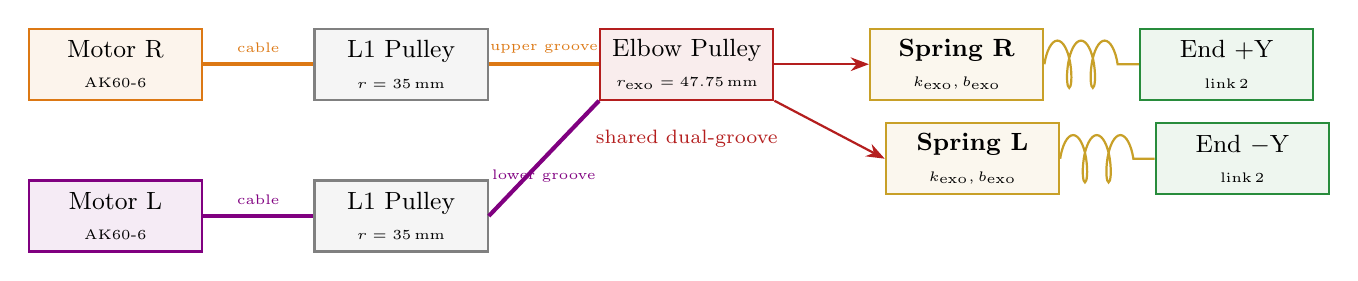
\begin{tikzpicture}[
    >=Stealth,
    block/.style={rectangle, draw=#1, thick, fill=#1!8,
                  minimum height=0.9cm, minimum width=2.2cm, align=center, font=\small},
    spring/.style={decorate, decoration={coil, aspect=0.3, segment length=3mm, amplitude=3mm}},
    cable/.style={line width=1.5pt, #1},
    arr/.style={-Stealth, thick, #1},
]
    % Right (upper groove) cable path
    \node[block=seaorange] (motorR) {Motor R\\{\tiny AK60-6}};
    \node[block=gray, right=1.4cm of motorR] (link1R) {L1 Pulley\\{\tiny $r = 35$\,mm}};
    \node[block=darkred, right=1.4cm of link1R] (elbow) {Elbow Pulley\\{\tiny $r_{\mathrm{exo}} = 47.75$\,mm}};
    \node[block=springgold, right=1.2cm of elbow] (springR) {\textbf{Spring R}\\{\tiny $k_{\mathrm{exo}}, b_{\mathrm{exo}}$}};
    \node[block=drakegreen, right=1.2cm of springR] (endR) {End +Y\\{\tiny link\,2}};

    \draw[cable=seaorange] (motorR.east) -- (link1R.west) node[midway, above, font=\tiny] {cable};
    \draw[cable=seaorange] (link1R.east) -- (elbow.west) node[midway, above, font=\tiny] {upper groove};
    \draw[arr=darkred] (elbow.east) -- (springR.west);
    \draw[spring, thick, springgold] (springR.east) -- (endR.west);

    % Left (lower groove) cable path — below
    \node[block=violet, below=1.0cm of motorR] (motorL) {Motor L\\{\tiny AK60-6}};
    \node[block=gray, right=1.4cm of motorL] (link1L) {L1 Pulley\\{\tiny $r = 35$\,mm}};
    \node[block=springgold, right=1.4cm of elbow, yshift=-1.2cm] (springL) {\textbf{Spring L}\\{\tiny $k_{\mathrm{exo}}, b_{\mathrm{exo}}$}};
    \node[block=drakegreen, right=1.2cm of springL] (endL) {End $-$Y\\{\tiny link\,2}};

    \draw[cable=violet] (motorL.east) -- (link1L.west) node[midway, above, font=\tiny] {cable};
    \draw[cable=violet] (link1L.east) -- (elbow.south west) node[midway, below, font=\tiny] {lower groove};
    \draw[arr=darkred] (elbow.south east) -- (springL.west);
    \draw[spring, thick, springgold] (springL.east) -- (endL.west);

    % Labels
    \node[below=0.25cm of elbow, font=\scriptsize, text=darkred] {shared dual-groove};
\end{tikzpicture}
\end{center}
\end{archbox}

The two cables are routed on \textbf{separate Z-planes} (3\,mm apart) through the same elbow pulley.
The \textbf{right/orange cable} (upper groove) wraps from the $-Y$ motor start, through a link-1 idler, crosses via an \emph{internal tangent} to the $+Y$ side, and terminates at the link-2 anchor.
The \textbf{left/purple cable} (lower groove) mirrors this on the opposite side.

Because the elbow pulley is centred on the joint axis, the moment arm is \textbf{constant}:
$l_c' = r_{\mathrm{exo}}$ for all $q_2$.


\subsection{Exosuit State Variables}

The exosuit adds \textbf{four motor-side state variables} (two per antagonistic channel):

\begin{table}[H]
\centering
\caption{Exosuit discrete state vector (6D).}
\begin{tabular}{clcl}
\toprule
\textbf{Symbol} & \textbf{Description} & \textbf{Units} & \textbf{Index} \\
\midrule
$\theta_{\mathrm{m,R}}$ & Right motor rotor angle & rad & 0 \\
$\dot{\theta}_{\mathrm{m,R}}$ & Right motor angular velocity & rad/s & 1 \\
$\theta_{\mathrm{m,L}}$ & Left motor rotor angle & rad & 2 \\
$\dot{\theta}_{\mathrm{m,L}}$ & Left motor angular velocity & rad/s & 3 \\
$q_2^{\dagger}$ & Elbow angle captured at activation (anchor) & rad & 4 \\
\texttt{was\_active} & Activation flag from previous timestep & bool & 5 \\
\bottomrule
\end{tabular}
\end{table}

\begin{warnbox}
\textbf{Motor-side angles.}
$\theta_{\mathrm{m,R}}$ and $\theta_{\mathrm{m,L}}$ are motor-side (before the gearbox).
The joint-side equivalent is $\theta_{\mathrm{m}} / N$.
\end{warnbox}


\subsection{Spring Extensions and Cable Forces}
\label{sec:exo_spring}

\subsubsection{Right Cable (Upper Groove)}
The right cable wraps so that positive motor motion drives $+q_2$:
\begin{equation}
\boxed{\delta_R = r_{\mathrm{exo}} \!\left(\frac{\theta_{\mathrm{m,R}}}{N} - q_2\right)}
\label{eq:delta_R}
\end{equation}
\begin{equation}
    \dot{\delta}_R = r_{\mathrm{exo}} \!\left(\frac{\dot{\theta}_{\mathrm{m,R}}}{N} - \dot{q}_2\right)
\label{eq:delta_R_dot}
\end{equation}

\subsubsection{Left Cable (Lower Groove)}
The left cable wraps in the opposite direction (virtual joint $= -q_2$):
\begin{equation}
\boxed{\delta_L = r_{\mathrm{exo}} \!\left(\frac{\theta_{\mathrm{m,L}}}{N} + q_2\right)}
\label{eq:delta_L}
\end{equation}
\begin{equation}
    \dot{\delta}_L = r_{\mathrm{exo}} \!\left(\frac{\dot{\theta}_{\mathrm{m,L}}}{N} + \dot{q}_2\right)
\label{eq:delta_L_dot}
\end{equation}

\subsubsection{Unilateral Cable Forces}
Cables can only pull ($T \geq 0$):
\begin{equation}
\boxed{
    F_R = \max\!\bigl(k_{\mathrm{exo}}\,\delta_R + b_{\mathrm{exo}}\,\dot{\delta}_R,\;0\bigr), \qquad
    F_L = \max\!\bigl(k_{\mathrm{exo}}\,\delta_L + b_{\mathrm{exo}}\,\dot{\delta}_L,\;0\bigr)
}
\label{eq:exo_forces}
\end{equation}


\subsection{Net Exosuit Torque}

Using the virtual-work signs ($\partial\delta_R / \partial q_2 = -r_{\mathrm{exo}}$, $\partial\delta_L / \partial q_2 = +r_{\mathrm{exo}}$):
\begin{equation}
\boxed{\tau_{\mathrm{exo}} = r_{\mathrm{exo}} \cdot (F_R - F_L)}
\label{eq:tau_exo}
\end{equation}

Joint~2 receives the \textbf{sum} of drive and exo torques:
\begin{equation}
    \tau_2^{\mathrm{total}} = \underbrace{\rp \cdot F_{\mathrm{cable}}}_{\text{drive SEA}} + \underbrace{r_{\mathrm{exo}} (F_R - F_L)}_{\text{exosuit}}
\label{eq:tau2_total}
\end{equation}


\subsection{Motor Encoder Tracking (Torque Mode)}
\label{sec:exo_motor}

Each exo motor uses the same 2nd-order MIT torque-mode rotor dynamics as the
drive SEA (Section~\ref{sec:torque_mode}), but the \textbf{motor command} is
generated by an internal \textbf{PD encoder-tracking} law rather than by the
CT controller.

The exosuit has two operating modes, selectable at runtime:

% ── MODE 1 ─────────────────────────────────────────────────────────────────
\subsubsection{Mode~1: Transparency (Deactivated)}
\label{sec:exo_transparent}

When deactivated ($\Delta\theta = 0$), both motors continuously track the
elbow encoder so that each spring extension stays at zero:
\begin{align}
    q_{\mathrm{des,R}} &=  q_2   &  \dot{q}_{\mathrm{des,R}} &=  \dot{q}_2 \notag\\
    q_{\mathrm{des,L}} &= -q_2   &  \dot{q}_{\mathrm{des,L}} &= -\dot{q}_2
\label{eq:exo_deactivated}
\end{align}

\textbf{What happens physically:}
As the elbow moves (driven by the CT+SEA pipeline), the PD tracker keeps each
motor angle at $\theta_{\mathrm{m,R}}/N \approx q_2$ and
$\theta_{\mathrm{m,L}}/N \approx -q_2$.  The spring extensions therefore
remain:
\[
    \delta_R = r_{\mathrm{exo}}\!\left(\frac{\theta_{\mathrm{m,R}}}{N} - q_2\right) \approx 0, \qquad
    \delta_L = r_{\mathrm{exo}}\!\left(\frac{\theta_{\mathrm{m,L}}}{N} + q_2\right) \approx 0
\]
Because $\delta \approx 0$ in both cables, $F_R \approx 0$ and $F_L \approx 0$, giving
$\tau_{\mathrm{exo}} \approx 0$.

\begin{resultbox}
\textbf{Transparency means zero additional stiffness.}
The exosuit does not resist the elbow motion at all.  The motors ``follow''
the joint, paying out and taking up cable exactly as fast as the elbow moves.
The robot behaves as if the exosuit were not present.
\end{resultbox}

In practice, transparency is imperfect: the PD tracker has finite bandwidth,
so at high joint velocities there is a small transient $\delta \neq 0$ (and
hence a small parasitic torque).  With $K_P = 200$\,Nm/rad and
$\omega_{\mathrm{pd}} \approx 450$\,rad/s this residual is negligible for
typical trajectory speeds ($\dot{q}_2 < 5$\,rad/s).


% ── MODE 2 ─────────────────────────────────────────────────────────────────
\subsubsection{Mode~2: Activated (Co-Contraction)}
\label{sec:exo_activated}

When activated, a symmetric angular offset $\Delta\theta > 0$ is added to
both motor targets.  The reference is the CT \textbf{desired} joint angle
$q_{2,\mathrm{des}}$ (from the trajectory IK), not the actual $q_2$
(see Section~\ref{sec:exo_qdes} for the rationale):
\begin{align}
    q_{\mathrm{des,R}} &=  q_{2,\mathrm{des}} + \Delta\theta  &  \dot{q}_{\mathrm{des,R}} &=  \dot{q}_{2,\mathrm{des}} \notag\\
    q_{\mathrm{des,L}} &= -q_{2,\mathrm{des}} + \Delta\theta  &  \dot{q}_{\mathrm{des,L}} &= -\dot{q}_{2,\mathrm{des}}
\label{eq:exo_activated}
\end{align}

\textbf{What happens physically:}
Both motors advance \emph{beyond} the CT desired joint state by
$\Delta\theta$.  Each motor pays out (or retracts) extra cable
$r_{\mathrm{exo}}\,\Delta\theta$ metres, pretensioning its spring.

When the motors have converged, the steady-state extensions are:
\begin{align}
    \delta_R^{\mathrm{ss}} &= r_{\mathrm{exo}}\,\Delta\theta > 0
        & &\Longrightarrow & F_R &= k_{\mathrm{exo}}\,r_{\mathrm{exo}}\,\Delta\theta > 0 \notag\\
    \delta_L^{\mathrm{ss}} &= r_{\mathrm{exo}}\,\Delta\theta > 0
        & &\Longrightarrow & F_L &= k_{\mathrm{exo}}\,r_{\mathrm{exo}}\,\Delta\theta > 0
\label{eq:pretension}
\end{align}
Both cables carry \textbf{equal pre-tension}.  Since $F_R = F_L$, the net
torque is:
\[
    \tau_{\mathrm{exo}}^{\mathrm{ss}}
      = r_{\mathrm{exo}}(F_R - F_L) = 0
\]
At the nominal position the exosuit adds \textbf{no net torque}; it only
creates latent stiffness that activates when the joint is disturbed.


% ── q_des REFERENCE PORT ────────────────────────────────────────────────────
\subsubsection{Motor Reference Port: Tracking $q_{2,\mathrm{des}}$}
\label{sec:exo_qdes}

\texttt{SEAExoActuator} exposes a \textbf{\texttt{q\_des}} input port (2-element
vector) that, when connected, supplies the CT controller's desired joint
positions as the motor reference in activated mode.

\begin{lstlisting}[language=Python, style=python,
    caption={Drake diagram wiring: CT desired positions to exosuit reference.}]
# In run_simulation() after building CT and exo systems:
builder.Connect(
    ct.GetOutputPort("joint_positions"),   # 2D: [q1_des, q2_des]
    exo.GetInputPort("q_des"),
)
\end{lstlisting}

The anchor logic inside \texttt{\_update\_motors()} selects the reference
depending on mode:
\begin{lstlisting}[language=Python, style=python,
    caption={Reference selection in \texttt{SEAExoActuator.\_update\_motors()}.}]
if activated:
    if self._qdes_port.HasValue(context):
        q_des_vec = self._qdes_port.Eval(context)
        q2_ref = float(q_des_vec[1])   # track q2_des (CT reference)
    else:
        q2_ref = q2_anchor             # fallback: frozen anchor
else:
    q2_ref = q2                        # transparent: follow actual joint

q_des_R =  q2_ref + delta_theta       # right motor target (joint side)
q_des_L = -q2_ref + delta_theta       # left motor target (joint side)
\end{lstlisting}

\begin{table}[H]
\centering
\caption{Motor reference selection by mode.}
\begin{tabular}{llll}
\toprule
\textbf{Mode} & \textbf{$q_{2,\mathrm{ref}}$} & \textbf{Spring behaviour} & \textbf{$\tau_{\mathrm{exo}}$} \\
\midrule
Transparent (off) & $q_2$ (actual) & $\delta \approx 0$ at all times & $\approx 0$ \\
Activated (on, \texttt{q\_des} connected) & $q_{2,\mathrm{des}}$ (CT) & $\delta = r_{\mathrm{exo}}(\pm\Delta\theta \mp (q_2-q_{2,\mathrm{des}}))$ & $-k_{\mathrm{eff}}(q_2 - q_{2,\mathrm{des}})$ \\
Activated (on, fallback) & $q_2^{\dagger}$ (frozen anchor) & spring pulls back to activation pose & large, fights CT \\
\bottomrule
\end{tabular}
\end{table}

\begin{resultbox}
\textbf{Why $q_{2,\mathrm{des}}$ instead of $q_2$?}

If the reference were the \emph{actual} $q_2$, the motor targets would follow
the joint, and the spring extensions would stay near $\pm r_{\mathrm{exo}}\Delta\theta$
even during trajectory motion.  No net torque would be produced except
transiently (relying on motor lag).

With $q_{2,\mathrm{des}}$:
\begin{itemize}[leftmargin=2em, itemsep=1pt]
    \item During \textbf{clean tracking} ($q_2 \approx q_{2,\mathrm{des}}$):
          $\tau_{\mathrm{exo}} \approx 0$ --- exosuit is transparent.
    \item During a \textbf{disturbance} ($q_2 \neq q_{2,\mathrm{des}}$):
          $\tau_{\mathrm{exo}} = -k_{\mathrm{eff}}(q_2 - q_{2,\mathrm{des}})$
          acts \emph{immediately}, without relying on motor bandwidth lag.
    \item The exosuit provides \emph{elastic stiffness} around the CT reference
          trajectory, not around a fixed pose.
\end{itemize}
\end{resultbox}


% ── DISTURBANCE REJECTION ─────────────────────────────────────────────────
\subsubsection{Disturbance Rejection: Restoring the Elbow}
\label{sec:exo_disturbance}

\paragraph{Key insight.}
The motor targets track the CT \emph{desired} joint angle $q_{2,\mathrm{des}}$
(from the trajectory planner and IK solver), \textbf{not} the actual joint
angle $q_2$.  When a disturbance deflects $q_2$ away from $q_{2,\mathrm{des}}$,
the motor targets do \textbf{not change}---they remain anchored to the CT
reference.  The joint moves while the motors stay in place, immediately
creating asymmetric spring extensions proportional to the deflection:
\[
    \tau_{\mathrm{exo}} = -k_{\mathrm{eff}}\,(q_2 - q_{2,\mathrm{des}})
\]
This acts as a direct \textbf{elastic stiffness} around the CT trajectory
reference---no motor bandwidth lag required.

\begin{warnbox}
\textbf{Contrast with earlier implementations.}

An earlier version of the code used a \emph{frozen anchor}
$q_2^{\dagger}$ captured at the moment of activation:
\[
    q_{\mathrm{des,R}} = q_2^{\dagger} + \Delta\theta \quad\text{(original bug)}
\]
This caused the exosuit to behave as a stiff spring anchored to the
\emph{activation pose}, creating large continuous $\tau_{\mathrm{exo}}$
that fought the CT controller whenever the arm moved away from the activation
configuration (e.g.\ on circular or rectangular trajectories).
The current fix replaces the frozen anchor with $q_{2,\mathrm{des}}$ from
the CT's \texttt{joint\_positions} output port
(Section~\ref{sec:exo_qdes}).
\end{warnbox}

\bigskip
% ── PRE-CONDITION ────────────────────────────────────────────────────────────
\paragraph{Pre-condition: nominal steady state at $q_2^{*}$.}

In the activated mode the motor targets are:
\begin{equation}
    q_{\mathrm{des,R}} = q_2^{*} + \Delta\theta, \qquad
    q_{\mathrm{des,L}} = -q_2^{*} + \Delta\theta
\label{eq:nom_targets}
\end{equation}

Once the motors have converged, their joint-side positions equal the targets:
\begin{equation}
    \frac{\theta_{\mathrm{m,R}}}{N} = q_2^{*} + \Delta\theta, \qquad
    \frac{\theta_{\mathrm{m,L}}}{N} = -q_2^{*} + \Delta\theta
\label{eq:nom_motors}
\end{equation}

Substituting into the spring extension formulae (Eqs.~\ref{eq:delta_R}
and~\ref{eq:delta_L}) at $q_2 = q_2^{*}$:
\begin{align}
    \delta_R^{\mathrm{ss}}
      &= r_{\mathrm{exo}}\!\left(\frac{\theta_{\mathrm{m,R}}}{N} - q_2^{*}\right)
       = r_{\mathrm{exo}}\bigl[(q_2^{*}+\Delta\theta)-q_2^{*}\bigr]
       = r_{\mathrm{exo}}\,\Delta\theta
    \label{eq:nom_deltaR}\\[4pt]
    \delta_L^{\mathrm{ss}}
      &= r_{\mathrm{exo}}\!\left(\frac{\theta_{\mathrm{m,L}}}{N} + q_2^{*}\right)
       = r_{\mathrm{exo}}\bigl[(-q_2^{*}+\Delta\theta)+q_2^{*}\bigr]
       = r_{\mathrm{exo}}\,\Delta\theta
    \label{eq:nom_deltaL}
\end{align}

Both springs carry the same stretch $r_{\mathrm{exo}}\,\Delta\theta$, so:
\begin{equation}
    F_R^{\mathrm{ss}} = k_{\mathrm{exo}}\,r_{\mathrm{exo}}\,\Delta\theta
    = F_L^{\mathrm{ss}}
\end{equation}

The net exo torque at the nominal position is therefore \textbf{zero}:
\begin{equation}
    \tau_{\mathrm{exo}}^{\mathrm{ss}}
      = r_{\mathrm{exo}}\!\left(F_R^{\mathrm{ss}} - F_L^{\mathrm{ss}}\right) = 0
\label{eq:tau_nom_zero}
\end{equation}

\begin{resultbox}
\textbf{Preloaded but balanced.}
At the nominal joint position both cables carry equal tension
$F_0 = k_{\mathrm{exo}}\,r_{\mathrm{exo}}\,\Delta\theta > 0$ and the net
joint torque is zero.  The exosuit is preloaded --- both springs are stretched
--- but the antagonistic torques cancel perfectly.
\end{resultbox}

\bigskip
% ── DISTURBANCE ─────────────────────────────────────────────────────────────
\paragraph{Disturbance event.}

An external force pushes the elbow from $q_2^{*}$ to
$q_2 = q_2^{*} + \Delta q$ with $\Delta q > 0$ (further flexion).

\bigskip
% ── STEP 1 ──────────────────────────────────────────────────────────────────
\textbf{Step~1 --- Motor targets remain anchored to the CT reference $q_{2,\mathrm{des}}$.}

Because the motor reference is $q_{2,\mathrm{des}}$ (set by the trajectory, not
the actual joint), the disturbance \emph{does not change} the motor targets:
\begin{equation}
    q_{\mathrm{des,R}} = q_2^{*} + \Delta\theta, \qquad
    q_{\mathrm{des,L}} = -q_2^{*} + \Delta\theta
\label{eq:new_targets}
\end{equation}
where $q_2^* = q_{2,\mathrm{des}}$ is the CT desired angle (unchanged by the
disturbance).

The motors, already converged to the nominal positions, remain:
\begin{equation}
    \frac{\theta_{\mathrm{m,R}}}{N} \approx q_2^{*}+\Delta\theta, \qquad
    \frac{\theta_{\mathrm{m,L}}}{N} \approx -q_2^{*}+\Delta\theta
\label{eq:motors_still_nominal}
\end{equation}

The restoring torque arises \emph{immediately} (not through motor lag): as soon
as $q_2$ deviates from $q_2^* = q_{2,\mathrm{des}}$, the spring extensions
become asymmetric.

\bigskip
% ── STEP 2 ──────────────────────────────────────────────────────────────────
\textbf{Step~2 --- Spring extensions become asymmetric.}

With the joint at $q_2 = q_2^{*}+\Delta q$ and the motors still at their
nominal positions (Eq.~\ref{eq:motors_still_nominal}):

\medskip
\emph{Right cable}:
\begin{align}
    \delta_R
      &= r_{\mathrm{exo}}\!\left(\frac{\theta_{\mathrm{m,R}}}{N} - q_2\right)
       = r_{\mathrm{exo}}\bigl[(q_2^{*}+\Delta\theta)-(q_2^{*}+\Delta q)\bigr] \notag\\
      &= r_{\mathrm{exo}}(\Delta\theta - \Delta q)
       \quad \underbrace{\vphantom{X}< r_{\mathrm{exo}}\,\Delta\theta}_{\text{right unloads}}
    \label{eq:dist_deltaR}
\end{align}

\emph{Left cable}:
\begin{align}
    \delta_L
      &= r_{\mathrm{exo}}\!\left(\frac{\theta_{\mathrm{m,L}}}{N} + q_2\right)
       = r_{\mathrm{exo}}\bigl[(-q_2^{*}+\Delta\theta)+(q_2^{*}+\Delta q)\bigr] \notag\\
      &= r_{\mathrm{exo}}(\Delta\theta + \Delta q)
       \quad \underbrace{\vphantom{X}> r_{\mathrm{exo}}\,\Delta\theta}_{\text{left loads more}}
    \label{eq:dist_deltaL}
\end{align}

\begin{center}
\begin{tabular}{lcc}
\toprule
& \textbf{Before disturbance} & \textbf{After disturbance ($\Delta q > 0$)} \\
\midrule
$\delta_R$ & $r_{\mathrm{exo}}\,\Delta\theta$ & $r_{\mathrm{exo}}(\Delta\theta - \Delta q)\;\downarrow$ \\
$\delta_L$ & $r_{\mathrm{exo}}\,\Delta\theta$ & $r_{\mathrm{exo}}(\Delta\theta + \Delta q)\;\uparrow$ \\
$F_R - F_L$ & $0$ (balanced) & $-2\,k_{\mathrm{exo}}\,r_{\mathrm{exo}}\,\Delta q < 0$ \\
\bottomrule
\end{tabular}
\end{center}

\bigskip
% ── STEP 3 ──────────────────────────────────────────────────────────────────
\textbf{Step~3 --- Full derivation of the restoring torque.}

Assuming both cables remain taut ($|\Delta q| < \Delta\theta$), the cable forces are:
\begin{align}
    F_R &= k_{\mathrm{exo}}\,\delta_R = k_{\mathrm{exo}}\,r_{\mathrm{exo}}\,(\Delta\theta - \Delta q)
    \label{eq:FR_disturbed}\\[4pt]
    F_L &= k_{\mathrm{exo}}\,\delta_L = k_{\mathrm{exo}}\,r_{\mathrm{exo}}\,(\Delta\theta + \Delta q)
    \label{eq:FL_disturbed}
\end{align}

Net exo torque (expanding fully so all terms are visible):
\begin{align}
    \tau_{\mathrm{exo}}
      &= r_{\mathrm{exo}}\,(F_R - F_L) \notag\\
      &= r_{\mathrm{exo}}\Bigl[k_{\mathrm{exo}}\,r_{\mathrm{exo}}(\Delta\theta-\Delta q)
                              - k_{\mathrm{exo}}\,r_{\mathrm{exo}}(\Delta\theta+\Delta q)\Bigr]\notag\\
      &= k_{\mathrm{exo}}\,r_{\mathrm{exo}}^{2}\,
         \bigl[\underbrace{(\Delta\theta - \Delta q) - (\Delta\theta + \Delta q)}_{\Delta\theta\text{ cancels}}\bigr]\notag\\
      &= k_{\mathrm{exo}}\,r_{\mathrm{exo}}^{2}\,(-2\,\Delta q)
\end{align}

\begin{equation}
\boxed{\tau_{\mathrm{exo}} = -2\,k_{\mathrm{exo}}\,r_{\mathrm{exo}}^2\;\Delta q
                           = -k_{\mathrm{eff}}\;\Delta q}
\label{eq:restoring}
\end{equation}

\begin{warnbox}
\textbf{Why does $\Delta\theta$ vanish from the restoring torque?}

$\Delta\theta$ creates equal preload on \emph{both} cables.  When you compute
the \emph{difference} $F_R - F_L$, the common preload cancels exactly.  The
incremental restoring force comes only from the change in imbalance, which is
driven by $\Delta q$, not by $\Delta\theta$.

Consequence: $\Delta\theta$ is necessary to keep both cables taut (prevents
slack), but it does not set the restoring stiffness.  Only $k_{\mathrm{exo}}$
and $r_{\mathrm{exo}}$ determine $k_{\mathrm{eff}}$.
\end{warnbox}

\bigskip
% ── STEP 4 ──────────────────────────────────────────────────────────────────
\textbf{Step~4 --- The elbow returns to nominal.}

The restoring torque $\tau_{\mathrm{exo}} = -k_{\mathrm{eff}}\,\Delta q$
acts on the joint \emph{in addition to} whatever the CT+SEA pipeline
already provides.  It accelerates the elbow back toward $q_2^{*}$.

Simultaneously, the motor PD trackers update $\theta_{\mathrm{m}}$ toward the
new (displaced) targets (Eq.~\ref{eq:new_targets}).  As the elbow returns
($\Delta q \to 0$) two things happen together:
\begin{itemize}[leftmargin=2em]
    \item the spring asymmetry disappears: $\delta_R \to \delta_L \to r_{\mathrm{exo}}\Delta\theta$,
    \item the restoring torque fades: $\tau_{\mathrm{exo}} \to 0$.
\end{itemize}

The motors converge to their now-updated targets \emph{after} the joint
returns, re-establishing the symmetric preload at the new nominal trajectory
point.

\begin{resultbox}
\textbf{Disturbance rejection --- full step-by-step.}
\begin{enumerate}[leftmargin=2em, itemsep=2pt]
    \item \textbf{Nominal}: both cables carry equal preload
          $F_0 = k_{\mathrm{exo}}\,r_{\mathrm{exo}}\,\Delta\theta$.
          Net torque $= 0$.
    \item \textbf{Disturbance} displaces $q_2$ by $\Delta q > 0$.
    \item \textbf{Motors lag}: joint moves, motors are still at old positions.
    \item \textbf{Asymmetric stretch}: right cable unloads
          ($\delta_R \downarrow$), left cable loads ($\delta_L \uparrow$).
    \item \textbf{Restoring torque}:
          $\tau_{\mathrm{exo}} = -k_{\mathrm{eff}}\,\Delta q$ (opposes displacement).
    \item \textbf{Return}: exo torque drives elbow back; as $\Delta q \to 0$,
          $\tau_{\mathrm{exo}} \to 0$ and symmetric preload is restored.
\end{enumerate}
\textbf{Analogy:} two preloaded antagonistic muscles around the elbow joint.
If the arm is pushed, one muscle tightens and the other relaxes; the net
difference restores the arm.
\end{resultbox}

% ── SLACK LIMIT ─────────────────────────────────────────────────────────────
\begin{warnbox}
\textbf{Cable slack limit.}
The linear law (Eq.~\ref{eq:restoring}) holds only while \textbf{both cables
remain taut}, i.e.\ $\delta_R \geq 0 \Rightarrow \Delta q \leq \Delta\theta$.
If the disturbance is large enough to slack one cable, the piecewise torque
law applies:
\[
    \tau_{\mathrm{exo}} =
    \begin{cases}
        -k_{\mathrm{eff}}\,\Delta q
          & |\Delta q| \leq \Delta\theta \quad\text{(bilateral stiffness)} \\[6pt]
        +k_{\mathrm{exo}}\,r_{\mathrm{exo}}^{2}\,(\Delta\theta - \Delta q)
          & \Delta q > +\Delta\theta \quad\text{(right slack, left only)} \\[6pt]
        -k_{\mathrm{exo}}\,r_{\mathrm{exo}}^{2}\,(\Delta\theta + \Delta q)
          & \Delta q < -\Delta\theta \quad\text{(left slack, right only)}
    \end{cases}
\]
Beyond the slack threshold the effective stiffness halves and becomes
\textbf{unilateral}.  Increasing $\Delta\theta$ widens the bilateral zone
without changing its slope (since $k_{\mathrm{eff}}$ is independent of
$\Delta\theta$).
\end{warnbox}


\subsubsection{PD Tracking Torque (Joint Side)}

The motor torque command fed to each rotor is a saturated PD:
\begin{equation}
\boxed{
    \tau_{\mathrm{m},i} = \mathrm{clip}\!\Bigl(
        K_P\!\left(q_{\mathrm{des},i} - \frac{\theta_{\mathrm{m},i}}{N}\right)
      + K_D\!\left(\dot{q}_{\mathrm{des},i} - \frac{\dot{\theta}_{\mathrm{m},i}}{N}\right),\;
      -\tau_{\max},\; \tau_{\max}
    \Bigr)
}
\label{eq:exo_pd}
\end{equation}
where $K_P = 200$\,Nm/rad, $K_D = 2$\,Nm\,$\cdot$\,s/rad, $\tau_{\max} = 9$\,Nm (AK60-6 peak).

\subsubsection{Rotor Dynamics (Per Motor, Sub-Stepped)}

Each rotor integrates the same 2nd-order ODE as the drive motor
(Eq.~\ref{eq:torque_mode}):
\begin{equation}
    \Jm\,\ddot{\theta}_{\mathrm{m},i}
      = \frac{\tau_{\mathrm{m},i}}{N}
      - b_{\mathrm{m}}\,\dot{\theta}_{\mathrm{m},i}
      - \frac{r_{\mathrm{exo}} \cdot F_i}{N}
\label{eq:exo_rotor}
\end{equation}

\begin{warnbox}
\textbf{Sub-stepping is essential.}
The PD natural frequency $\omega_{\mathrm{pd}} = \sqrt{K_P / (\Jm N^2)} \approx 450$\,rad/s is much higher than the drive motor's spring resonance.
Without sub-stepping ($N_{\mathrm{sub}} = 10$ per $\Delta t$), the integrator becomes unstable.
\end{warnbox}


\subsection{Effective Co-Contraction Stiffness}
\label{sec:co_contraction}

When both exo motors track $q_2 \pm \Delta\theta$ perfectly, a small joint
perturbation $\Delta q$ from the current position produces:
\begin{align}
    \delta_R &= r_{\mathrm{exo}}(\Delta\theta - \Delta q)  \\
    \delta_L &= r_{\mathrm{exo}}(\Delta\theta + \Delta q)
\end{align}
so the restoring torque is:
\begin{align}
    \tau_{\mathrm{exo}} &= r_{\mathrm{exo}}\bigl(k_{\mathrm{exo}}\,r_{\mathrm{exo}}(\Delta\theta - \Delta q) - k_{\mathrm{exo}}\,r_{\mathrm{exo}}(\Delta\theta + \Delta q)\bigr) \notag \\
                        &= -2\,k_{\mathrm{exo}}\,r_{\mathrm{exo}}^2\,\Delta q
\end{align}

\begin{resultbox}
\textbf{Effective co-contraction stiffness:}
\begin{equation}
\boxed{k_{\mathrm{eff}} = 2\,k_{\mathrm{exo}}\,r_{\mathrm{exo}}^2}
\label{eq:keff}
\end{equation}
This is \textbf{independent of $\Delta\theta$} (the offset sets pre-tension, not stiffness) and \textbf{independent of $q_2$} (constant moment arm, Method~B).
\end{resultbox}

\begin{table}[H]
\centering
\caption{Effective stiffness for typical exo spring values ($r_{\mathrm{exo}} = 47.75$\,mm).}
\begin{tabular}{rr}
\toprule
$k_{\mathrm{exo}}$ [N/m] & $k_{\mathrm{eff}}$ [Nm/rad] \\
\midrule
60   & 0.27 \\
100  & 0.46 \\
200  & 0.91 \\
500  & 2.28 \\
\bottomrule
\end{tabular}
\end{table}


\subsection{Exosuit Parameters}

\begin{table}[H]
\centering
\caption{Default exosuit parameters (\texttt{SEAExoActuator} constructor).}
\begin{tabular}{llrl}
\toprule
\textbf{Parameter} & \textbf{Symbol} & \textbf{Default} & \textbf{Unit} \\
\midrule
\multicolumn{4}{l}{\textit{Cable \& Spring}} \\
Spring stiffness         & $k_{\mathrm{exo}}$         & 200       & N/m \\
Cable damping            & $b_{\mathrm{exo}}$         & 2.0       & N$\cdot$s/m \\
Elbow pulley radius      & $r_{\mathrm{exo}}$         & 47.75     & mm \\
\midrule
\multicolumn{4}{l}{\textit{Motor (CubeMars AK60-6, each)}} \\
Gear ratio               & $N$          & 6         & --- \\
Rotor inertia            & $\Jm$        & $3.32 \times 10^{-5}$  & kg$\cdot$m$^2$ \\
Viscous damping          & $\bmotor$    & derived   & N$\cdot$m$\cdot$s/rad \\
Peak torque              & $\tau_{\max}$& 9.0       & Nm \\
\midrule
\multicolumn{4}{l}{\textit{PD Tracking}} \\
Position gain            & $K_P$        & 200       & Nm/rad \\
Velocity gain            & $K_D$        & 2.0       & Nm$\cdot$s/rad \\
Sub-steps per $\Delta t$ & $N_{\mathrm{sub}}$ & 10 & --- \\
\midrule
\multicolumn{4}{l}{\textit{Activation}} \\
Co-contraction offset    & $\Delta\theta$ & 0.1    & rad \\
Activation time          & $t_{\mathrm{act}}$ & 5.0 & s \\
\bottomrule
\end{tabular}
\end{table}


\subsection{Exosuit Control Architecture}
\label{sec:exo_arch}

\begin{archbox}{Three-Layer Architecture: CT + Drive SEA + Exosuit}
\begin{center}
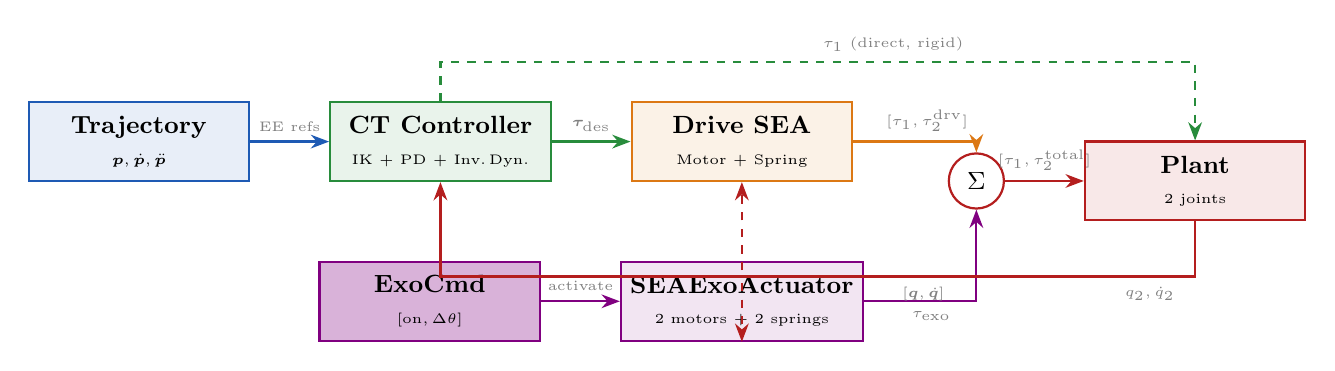
\begin{tikzpicture}[
    node distance=0.5cm and 0.8cm,
    block/.style={rectangle, draw=#1, thick, fill=#1!10!white,
                  minimum height=1cm, minimum width=2.8cm, align=center, font=\small},
    arr/.style={-Stealth, thick, #1},
    port/.style={font=\tiny, text=gray},
]
    % Block 1: CT
    \node[block=drakegreen] (ct) {\textbf{CT Controller}\\{\tiny IK + PD + Inv.\,Dyn.}};
    \node[block=drakeblue, left=1.0cm of ct] (traj) {\textbf{Trajectory}\\{\tiny $\bm{p}, \dot{\bm{p}}, \ddot{\bm{p}}$}};

    % Block 2: Drive SEA
    \node[block=seaorange, right=1.0cm of ct] (sea) {\textbf{Drive SEA}\\{\tiny Motor + Spring}};

    % Block 3: Exo
    \node[block=violet, below=1.0cm of sea] (exo) {\textbf{SEAExoActuator}\\{\tiny 2 motors + 2 springs}};
    \node[rectangle, draw=violet, thick, fill=violet!30!white,
          minimum height=1cm, minimum width=2.8cm, align=center, font=\small,
          left=1.0cm of exo] (cmd) {\textbf{ExoCmd}\\{\tiny $[\mathrm{on}, \Delta\theta]$}};

    % Summation → Plant
    \node[circle, draw=darkred, thick, inner sep=0pt, minimum size=7mm,
          right=1.2cm of sea, yshift=-0.5cm, font=\small] (sum) {$\Sigma$};
    \node[block=darkred, right=1.0cm of sum] (plant) {\textbf{Plant}\\{\tiny 2 joints}};

    % Wiring
    \draw[arr=drakeblue] (traj) -- (ct) node[midway, above, port] {EE refs};
    \draw[arr=drakegreen] (ct) -- (sea) node[midway, above, port] {$\btau_{\mathrm{des}}$};
    \draw[arr=seaorange] (sea.east) -| (sum) node[pos=0.3, above, port] {$[\tau_1, \tau_2^{\mathrm{drv}}]$};
    \draw[arr=violet] (exo.east) -| (sum) node[pos=0.3, below, port] {$\tau_{\mathrm{exo}}$};
    \draw[arr=darkred] (sum) -- (plant) node[midway, above, port] {$[\tau_1, \tau_2^{\mathrm{total}}]$};

    % Exo command
    \draw[arr=violet] (cmd) -- (exo) node[midway, above, port] {activate};

    % Feedback
    \draw[arr=darkred] (plant.south) -- ++(0,-0.7) -| (ct.south)
        node[pos=0.18, below, port] {$[\bq, \dot{\bq}]$};
    \draw[arr=darkred, dashed] (plant.south) -- ++(0,-0.7) -| (sea.south);
    \draw[arr=darkred, dashed] (plant.south) -- ++(0,-0.7) -| (exo.south)
        node[pos=0.05, below, port] {$q_2, \dot{q}_2$};

    % Direct τ₁ shortcut
    \draw[arr=drakegreen, dashed] (ct.north) -- ++(0,0.5) -| (plant.north)
        node[pos=0.3, above, port] {$\tau_1$ (direct, rigid)};
\end{tikzpicture}
\end{center}
\end{archbox}

\begin{warnbox}
\textbf{Additional wire (not shown):} the CT controller also sends
$q_{2,\mathrm{des}}$ to the exosuit via its \texttt{q\_des} input port
(Section~\ref{sec:exo_qdes}).  This allows the exosuit to track the desired
trajectory rather than a frozen anchor.
\end{warnbox}

\subsection{Detailed Signal-Flow Block Diagram (Exosuit Only)}
\label{sec:exo_block_diagram}

Figure~\ref{fig:exo_block_diagram} shows the signal-flow graph for a
\textbf{single exo motor--spring channel} (right cable shown; the left is
identical with virtual joint $-q_2$).

\begin{figure}[H]
\centering
\resizebox{\textwidth}{!}{%
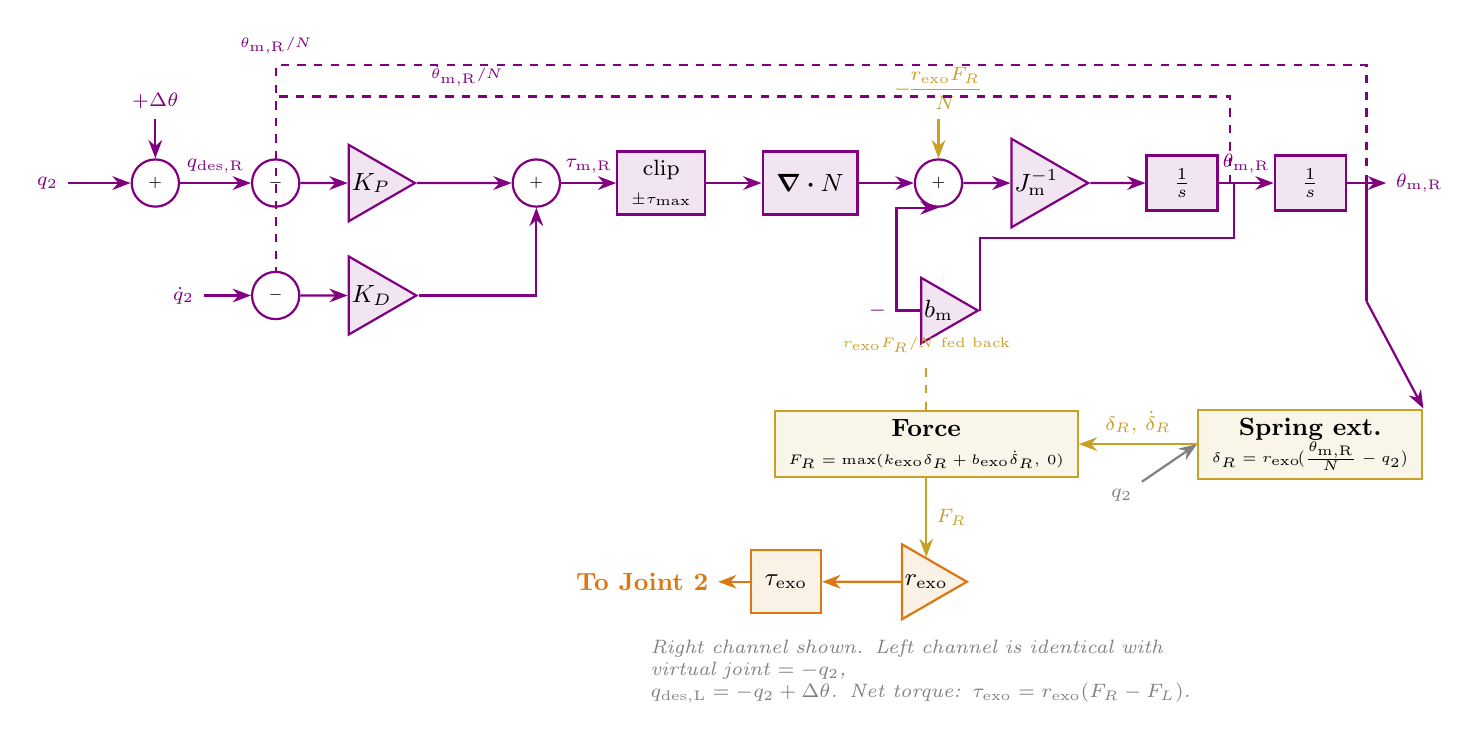
\begin{tikzpicture}[
    >=Stealth,
    sumnode/.style={circle, draw=#1, thick, inner sep=0pt,
                    minimum size=6mm, font=\scriptsize},
    block/.style={rectangle, draw=#1, thick, fill=#1!10!white,
                  minimum height=8mm, align=center, font=\small,
                  inner xsep=5pt, inner ysep=3pt},
    gain/.style={isosceles triangle, draw=#1, thick, fill=#1!10!white,
                 isosceles triangle apex angle=60,
                 minimum width=7mm, minimum height=5mm,
                 shape border rotate=0, font=\small, inner sep=1pt},
    integ/.style={rectangle, draw=violet, thick, fill=violet!10!white,
                  minimum height=7mm, minimum width=9mm,
                  align=center, font=\small},
    arr/.style={-Stealth, thick, #1},
    sig/.style={font=\scriptsize, text=#1},
    note/.style={font=\scriptsize\itshape, text=gray},
    groupbox/.style={draw=#1, thick, dashed, rounded corners=4pt,
                     fill=#1!4, inner sep=8pt},
]

% ── PD Tracking ──────────────────────────────────────────────────────────────
\node[sig=violet] (q2_in) {$q_2$};
\node[sumnode=violet, right=0.8cm of q2_in] (pd_sum_p) {};
\draw (pd_sum_p.center) node[font=\tiny] {$+$};
\node[above=0.5cm of pd_sum_p, sig=violet] (dtheta_in) {$+\Delta\theta$};
\draw[arr=violet] (q2_in) -- (pd_sum_p);
\draw[arr=violet] (dtheta_in) -- (pd_sum_p);

% position error
\node[sumnode=violet, right=0.9cm of pd_sum_p] (err_p) {};
\draw (err_p.center) node[font=\tiny] {$-$};
\draw[arr=violet] (pd_sum_p) -- (err_p)
    node[midway, above, sig=violet] {$q_{\mathrm{des,R}}$};

% Kp gain
\node[gain=violet, right=0.6cm of err_p] (Kp_exo) {$K_P$};
\draw[arr=violet] (err_p) -- (Kp_exo);

% Kd branch (velocity error, below)
\node[sumnode=violet, below=0.8cm of err_p] (err_v) {};
\draw (err_v.center) node[font=\tiny] {$-$};
\node[gain=violet, right=0.6cm of err_v] (Kd_exo) {$K_D$};
\draw[arr=violet] (err_v) -- (Kd_exo);

% velocity refs
\node[left=0.6cm of err_v, sig=violet] (qdot_des) {$\dot{q}_2$};
\draw[arr=violet] (qdot_des) -- (err_v);

% sum PD
\node[sumnode=violet, right=1.2cm of Kp_exo] (pd_out) {};
\draw (pd_out.center) node[font=\tiny] {$+$};
\draw[arr=violet] (Kp_exo) -- (pd_out);
\draw[arr=violet] (Kd_exo.east) -| (pd_out);

% clip
\node[block=violet, right=0.7cm of pd_out] (clip) {\footnotesize clip\\[-1pt]{\tiny $\pm\tau_{\max}$}};
\draw[arr=violet] (pd_out) -- (clip)
    node[midway, above, sig=violet] {$\tau_{\mathrm{m,R}}$};

% ── Rotor Dynamics ───────────────────────────────────────────────────────────
% ÷N
\node[block=violet, right=0.7cm of clip] (divN) {$\div N$};
\draw[arr=violet] (clip) -- (divN);

% Motor sum
\node[sumnode=violet, right=0.7cm of divN] (msum) {};
\draw (msum.center) node[font=\tiny] {$+$};
\draw[arr=violet] (divN) -- (msum);

% 1/Jm
\node[gain=violet, right=0.6cm of msum] (invJm) {$\Jm^{-1}$};
\draw[arr=violet] (msum) -- (invJm);

% Integrators
\node[integ, right=0.7cm of invJm] (int1) {$\frac{1}{s}$};
\draw[arr=violet] (invJm) -- (int1);
\node[integ, right=0.7cm of int1] (int2) {$\frac{1}{s}$};
\draw[arr=violet] (int1) -- (int2)
    node[midway, above, sig=violet] {$\dot{\theta}_{\mathrm{m,R}}$};
\node[right=0.5cm of int2, sig=violet] (thetam_out) {$\theta_{\mathrm{m,R}}$};
\draw[arr=violet] (int2) -- (thetam_out);

% b_m feedback
\coordinate (bm_fb) at ($(int1.east) + (0.2, 0)$);
\node[gain=violet, below=1.0cm of msum] (bm) {$\bmotor$};
\draw[violet, thick] (bm_fb) -- ++(0,-0.7) -| (bm.east);
\draw[arr=violet] (bm.west) -- ++(-0.3, 0) |- (msum.south)
    node[pos=0.0, left, sig=violet] {$-$};

% r_exo·F/N feedback
\node[above=0.5cm of msum, sig=springgold] (rpF_lab) {$-\!\dfrac{r_{\mathrm{exo}} F_R}{N}$};
\draw[arr=springgold] (rpF_lab) -- (msum.north);

% ── θ_m/N feedback to position error ─────────────────────────────────────
\coordinate (theta_fb) at ($(int2.east) + (0.25, 0)$);
\draw[violet, thick, dashed] (theta_fb) -- ++(0, 1.5) -| (err_p.north)
    node[pos=0.5, above, sig=violet] {\tiny $\theta_{\mathrm{m,R}}/N$};
% velocity feedback to Kd
\coordinate (thetadot_fb) at ($(int1.east) + (0.15, 0)$);
\draw[violet, thick, dashed] (thetadot_fb) -- ++(0, 1.1) -| (err_v.north)
    node[pos=0.4, above, sig=violet] {\tiny $\dot{\theta}_{\mathrm{m,R}}/N$};

% ── Spring & Force ───────────────────────────────────────────────────────────
\node[block=springgold, below=2.5cm of int2] (delta_blk)
    {\textbf{Spring ext.}\\[-1pt]{\tiny $\delta_R = r_{\mathrm{exo}}\!\bigl(\frac{\theta_{\mathrm{m,R}}}{N} - q_2\bigr)$}};

% θ_m → δ
\draw[violet, thick] ($(int2.east) + (0.25, 0)$) -- ++(0, -1.5);
\draw[arr=violet] ($(int2.east) + (0.25, -1.5)$) -- (delta_blk.north east);

% q₂ → δ
\node[below left=0.0cm and 0.7cm of delta_blk, sig=gray] (q2_delta) {$q_2$};
\draw[arr=gray] (q2_delta) -- (delta_blk.west);

% F = ks·δ + bc·δ̇
\node[block=springgold, left=1.5cm of delta_blk] (F_blk)
    {\textbf{Force}\\[-1pt]{\tiny $F_R = \max(k_{\mathrm{exo}}\delta_R + b_{\mathrm{exo}}\dot{\delta}_R,\,0)$}};
\draw[arr=springgold] (delta_blk) -- (F_blk)
    node[midway, above, sig=springgold] {$\delta_R,\,\dot{\delta}_R$};

% τ_exo = r_exo · (F_R - F_L)
\node[gain=seaorange, below=1.0cm of F_blk] (rp_exo) {$r_{\mathrm{exo}}$};
\draw[arr=springgold] (F_blk.south) -- (rp_exo.north)
    node[midway, right, sig=springgold] {$F_R$};

\node[block=seaorange, left=1.0cm of rp_exo] (tau_exo_out) {$\tau_{\mathrm{exo}}$};
\draw[arr=seaorange] (rp_exo) -- (tau_exo_out);
\node[left=0.4cm of tau_exo_out, sig=seaorange, font=\small\bfseries] (jt2_exo) {\textbf{To Joint 2}};
\draw[arr=seaorange] (tau_exo_out) -- (jt2_exo);

% Spring feedback to motor
\draw[springgold, thick, dashed] (F_blk.north) -- ++(0, 0.6)
    node[above, sig=springgold] {\tiny $r_{\mathrm{exo}} F_R / N$ fed back};

% ── Annotation ───────────────────────────────────────────────────────────────
\node[note, below=0.3cm of rp_exo, text width=7cm] {%
    Right channel shown.  Left channel is identical with virtual joint $=-q_2$,\\
    $q_{\mathrm{des,L}} = -q_2 + \Delta\theta$.  Net torque: $\tau_{\mathrm{exo}} = r_{\mathrm{exo}}(F_R - F_L)$.};

\end{tikzpicture}
}% end resizebox
\caption{Signal-flow block diagram for one exosuit motor--spring channel (right cable).
    A PD encoder-tracking law generates motor torque $\tau_{\mathrm{m,R}}$;
    the 2nd-order rotor integrates with viscous damping and spring-load
    feedback; the unilateral spring force $F_R$ maps through the elbow pulley
    radius to a torque contribution.  The left channel mirrors this with
    virtual joint $-q_2$.  The net exosuit torque is
    $\tau_{\mathrm{exo}} = r_{\mathrm{exo}}\,(F_R - F_L)$.}
\label{fig:exo_block_diagram}
\end{figure}


\subsection{Per-Timestep Algorithm (Torque Mode)}
\label{sec:exo_algorithm}

At each simulation step ($\Delta t = 2$\,ms), the exosuit executes in parallel
with the drive SEA (both read the same plant state):

\medskip
\textbf{Block~3 --- \texttt{SEAExoActuator}} (\texttt{actuators/sea\_exo.py}):
\begin{enumerate}[leftmargin=2em]
    \item \textbf{Read activation command}: \texttt{[on/off, $\Delta\theta$]}
    \item \textbf{Read joint state}: extract $(q_2, \dot{q}_2)$ from plant
    \item \textbf{Compute motor targets} (use $q_{2,\mathrm{des}}$ from \texttt{q\_des} port when
          activated; use $q_2$ when transparent):
    \[
        q_{\mathrm{des,R}} = q_{2,\mathrm{ref}} + \Delta\theta, \qquad
        q_{\mathrm{des,L}} = -q_{2,\mathrm{ref}} + \Delta\theta
    \]
    where $q_{2,\mathrm{ref}} = q_{2,\mathrm{des}}$ if activated, $q_2$ if transparent.
    \item \textbf{Sub-stepped loop} ($N_{\mathrm{sub}} = 10$ iterations):
        \begin{enumerate}[label=(\alph*)]
            \item PD tracking torque (Eq.~\ref{eq:exo_pd}): $\tau_{\mathrm{m},i}$ for each motor
            \item Rotor dynamics (Eq.~\ref{eq:exo_rotor}): update $[\theta_{\mathrm{m},i}, \dot{\theta}_{\mathrm{m},i}]$
        \end{enumerate}
    \item \textbf{Spring forces} (Eq.~\ref{eq:exo_forces}): $F_R$, $F_L$ (unilateral)
    \item \textbf{Net exo torque} (Eq.~\ref{eq:tau_exo}): $\tau_{\mathrm{exo}} = r_{\mathrm{exo}}(F_R - F_L)$
    \item \textbf{Clamp and output}: $\tau_{\mathrm{exo}} \gets \mathrm{clip}(\tau_{\mathrm{exo}}, -\tau_{\max}, \tau_{\max})$
\end{enumerate}

The output $\tau_{\mathrm{exo}}$ is summed with the drive torques in an
\texttt{ActuationSum} adder block before reaching the plant.


\subsection{Diagnostics Output}

The \texttt{diagnostics} output port exports a 10-element vector for logging
and plotting:

\begin{table}[H]
\centering
\caption{Exosuit diagnostics vector (10D).}
\begin{tabular}{clc}
\toprule
\textbf{Index} & \textbf{Quantity} & \textbf{Unit} \\
\midrule
0 & $\delta_R$ --- right spring extension  & m \\
1 & $\delta_L$ --- left spring extension   & m \\
2 & $F_R$ --- right cable force            & N \\
3 & $F_L$ --- left cable force             & N \\
4 & $\theta_{\mathrm{m,R}}/N$ --- right motor joint-side pos  & rad \\
5 & $\theta_{\mathrm{m,L}}/N$ --- left motor joint-side pos   & rad \\
6 & $\dot{\theta}_{\mathrm{m,R}}/N$ --- right motor joint-side vel  & rad/s \\
7 & $\dot{\theta}_{\mathrm{m,L}}/N$ --- left motor joint-side vel   & rad/s \\
8 & $\tau_{\mathrm{exo}}$ --- net exo torque  & Nm \\
9 & activated (1.0 or 0.0) & --- \\
\bottomrule
\end{tabular}
\end{table}


\subsection{Summary of Exosuit Equations}

\begin{archbox}{Exosuit Equation Summary (Torque Mode)}
\textbf{Motor target} (activated, reference = CT desired $q_{2,\mathrm{des}}$):
\begin{align*}
    q_{\mathrm{des,R}} &= q_{2,\mathrm{des}} + \Delta\theta &
    q_{\mathrm{des,L}} &= -q_{2,\mathrm{des}} + \Delta\theta
\end{align*}

\textbf{PD tracking}:
\[
    \tau_{\mathrm{m},i} = \mathrm{clip}\!\bigl(
        K_P(q_{\mathrm{des},i} - \theta_{\mathrm{m},i}/N)
      + K_D(\dot{q}_{\mathrm{des},i} - \dot{\theta}_{\mathrm{m},i}/N),\;
      \pm\tau_{\max}\bigr)
\]

\textbf{Rotor dynamics}:
\[
    \Jm\,\ddot{\theta}_{\mathrm{m},i}
      = \frac{\tau_{\mathrm{m},i}}{N}
      - b_{\mathrm{m}}\,\dot{\theta}_{\mathrm{m},i}
      - \frac{r_{\mathrm{exo}} F_i}{N}
\]

\textbf{Spring extensions}:
\[
    \delta_R = r_{\mathrm{exo}}\!\left(\frac{\theta_{\mathrm{m,R}}}{N} - q_2\right), \qquad
    \delta_L = r_{\mathrm{exo}}\!\left(\frac{\theta_{\mathrm{m,L}}}{N} + q_2\right)
\]

\textbf{Cable forces} (unilateral):
\[
    F_i = \max(k_{\mathrm{exo}}\,\delta_i + b_{\mathrm{exo}}\,\dot{\delta}_i,\; 0)
\]

\textbf{Net exo torque}:
\[
    \tau_{\mathrm{exo}} = r_{\mathrm{exo}} (F_R - F_L)
\]

\textbf{Effective stiffness} (co-contraction):
\[
    k_{\mathrm{eff}} = 2\,k_{\mathrm{exo}}\,r_{\mathrm{exo}}^2
\]
\end{archbox}


% ============================================================================
\section{Drake Implementation}
\label{sec:drake}
% ============================================================================

\subsection{Source File}

\texttt{script\_cup\_manipulator\_pendulam\_tendon\_with\_spring\_sea\_pydrake.py} ($\sim$900 lines) uses a \textbf{two-block architecture}: control logic in \texttt{ComputedTorqueController} and actuator physics in \texttt{SEACableActuator}, wired together via a Drake diagram.

\begin{table}[H]
\centering
\caption{Key classes and functions.}
\begin{tabular}{p{5.5cm}p{8cm}}
\toprule
\textbf{Name} & \textbf{Role} \\
\midrule
\texttt{ComputedTorqueController}     & Drake \texttt{LeafSystem} (controller/controller.py). IK + PD + inverse dynamics. Outputs $\btau_{\mathrm{des}}$. \\
\texttt{SEACableActuator}             & Drake \texttt{LeafSystem} (actuators/sea.py). Delegates to \texttt{MotorDynamics} + spring--damper cable model. \\
\texttt{MotorDynamics}                & ABC (actuators/motor\_dynamics.py). Subclasses: \texttt{TorqueMotor} (2nd-order), \texttt{PositionServoMotor} (1st-order). \\
\texttt{\_build\_rect\_trajectory} & C$^2$ rectangular EE trajectory with speed-profiled corners. \\
\texttt{\_build\_move\_to\_start}  & Cubic-Hermite approach preamble. \\
\texttt{run\_simulation()}        & Build, wire, run, collect logs for one SEA config. \\
\texttt{plot\_sea\_results()}     & 3$\times$3 diagnostic panel + EE path overlay. \\
\texttt{main()}                   & CLI dispatch, optional \texttt{--compare} mode. \\
\bottomrule
\end{tabular}
\end{table}

\subsection{SEACableActuator --- Pure Actuator LeafSystem}

The \texttt{SEACableActuator} (\texttt{actuators/sea.py}) is a pure physics model with no control law.  It accepts desired torques $[\tau_1, \tau_2]$ and outputs actual torques after motor + spring dynamics.  Motor dynamics are delegated to a pluggable \texttt{MotorDynamics} object (\texttt{actuators/motor\_dynamics.py}).

\begin{lstlisting}[caption={Motor dynamics class hierarchy (actuators/motor\_dynamics.py).}]
class MotorMode(Enum):
    TORQUE   = "torque"       # 2nd-order rotor dynamics (default)
    POSITION = "position"     # 1st-order position servo (legacy)

class MotorDynamics(ABC):            # shared interface
    def step(self, state, tau2_des, q2, q2_dot) -> np.ndarray: ...
    def compute_spring_force(self, state, ...) -> tuple: ...

class TorqueMotor(MotorDynamics):    # J_m * theta_ddot = tau_m - b_m * theta_dot - r_p*F/N
class PositionServoMotor(MotorDynamics):  # l_dot = omega_b * (l_des - l)
\end{lstlisting}

\begin{lstlisting}[caption={TorqueMotor: cable force in linear coordinates + semi-implicit Euler.}]
class TorqueMotor(MotorDynamics):
    def _cable_force_raw(self, theta_m, theta_m_dot, q2, q2_dot):
        delta_lin     = self._r_p * (theta_m / self._N - q2)
        delta_dot_lin = self._r_p * (theta_m_dot / self._N - q2_dot)
        F_raw = self._k_s * delta_lin + self._b_c * delta_dot_lin
        return F_raw, delta_lin

    def step(self, state, tau2_des, q2, q2_dot):
        theta_m, theta_m_dot = state[0], state[1]
        tau_m = tau2_des / self._N
        F_raw, _ = self._cable_force_raw(theta_m, theta_m_dot, q2, q2_dot)
        tau_spring_motor = self._r_p * F_raw / self._N
        theta_m_ddot = (tau_m - self._b_m * theta_m_dot
                        - tau_spring_motor) / self._J_m
        # Semi-implicit Euler (velocity first, then position)
        theta_m_dot_new = theta_m_dot + self._dt * theta_m_ddot
        theta_m_new     = theta_m     + self._dt * theta_m_dot_new
        return np.array([theta_m_new, theta_m_dot_new])
\end{lstlisting}

\begin{codemath}
\begin{align}
    \delta &= \rp \cdot (\thetam / N - q_2) \tag{spring extension [m]} \\
    \dot{\delta} &= \rp \cdot (\dot{\thetam} / N - \dot{q}_2) \tag{extension rate} \\
    F_{\mathrm{raw}} &= \ks \, \delta + \bc \, \dot{\delta} \tag{spring--damper} \\
    F_{\mathrm{cable}} &= T_{\mathrm{green}} - T_{\mathrm{red}} = F_{\mathrm{raw}} \tag{net antagonistic force}
\end{align}
\end{codemath}

\begin{lstlisting}[caption={SEACableActuator delegates to MotorDynamics (actuators/sea.py).}]
def _update_motor(self, context, discrete_state):
    motor_state = ... # read from Drake discrete state
    tau_des = self._tau_port.Eval(context)
    q, q_dot = self._read_joint_state(context)
    new_state = self._motor.step(motor_state, tau_des[1], q[1], q_dot[1])
    # write new_state back to Drake discrete state

def _calc_actuation(self, context, output):
    tau_des  = self._tau_port.Eval(context)
    motor_state = ... # read from Drake discrete state
    q, q_dot = self._read_joint_state(context)
    F_cable, _, _, _, _, _ = self._motor.compute_spring_force(
        motor_state, tau_des[1], q[1], q_dot[1])
    tau_out = np.array([
        tau_des[0],              # J1: pass-through (rigid)
        self._r_p * F_cable,     # J2: SEA cable spring
    ])
    output.SetFromVector(np.clip(tau_out, -self._tau_max, self._tau_max))
\end{lstlisting}

\begin{codemath}
\begin{align}
    \text{Torque mode:}\quad & \Jm \ddot{\thetam} = \tau_m - b_{\mathrm{m}} \dot{\thetam} - \rp F / N \tag{rotor EOM} \\
    \text{Position mode:}\quad & \lm[k{+}1] = \lm[k] + \Delta t \cdot \wb \cdot (\lm^{\mathrm{des}} - \lm[k]) \tag{motor servo} \\
    & \tau_1 = \tau_{1,\mathrm{des}} \tag{rigid J1} \\
    & \tau_2 = \rp \cdot F_{\mathrm{cable}} \tag{SEA J2}
\end{align}
\end{codemath}


\subsection{Diagnostics Output Port}

The \texttt{SEACableActuator} exposes an 8-element diagnostics vector for logging:

\begin{table}[H]
\centering
\caption{Diagnostics vector layout (8 elements).  Slots 0--1 depend on motor mode.}
\begin{tabular}{clcll}
\toprule
\textbf{Idx} & \textbf{Name} & \textbf{Symbol} & \textbf{Torque mode} & \textbf{Position mode} \\
\midrule
0 & Motor state (primary)   & --- & $\thetam / N$ [rad] & $\lm$ [m] \\
1 & Motor state (secondary) & --- & $\dot{\thetam} / N$ [rad/s] & $\lm^{\mathrm{des}}$ [m] \\
2 & Spring extension & $\delta$ & \multicolumn{2}{c}{m} \\
3 & Net cable force & $F_{\mathrm{cable}}$ & \multicolumn{2}{c}{N} \\
4 & CT desired $\tau_1$ & $\tau_{1,\mathrm{des}}$ & \multicolumn{2}{c}{Nm} \\
5 & CT desired $\tau_2$ & $\tau_{2,\mathrm{des}}$ & \multicolumn{2}{c}{Nm} \\
6 & Green cable tension & $T_{\mathrm{green}}$ & \multicolumn{2}{c}{N} \\
7 & Red cable tension & $T_{\mathrm{red}}$ & \multicolumn{2}{c}{N} \\
\bottomrule
\end{tabular}
\end{table}


% ============================================================================
\section{Spring Visualization}
\label{sec:viz}
% ============================================================================

The Meshcat 3D visualization draws the cable routing with pulleys, straight cable segments, and a helical spring coil on the last segment of each cable route.

\subsection{Dynamic Spring Length}

The spring visualization dynamically reflects the actual physics state.  The helper function \texttt{draw\_cables()} in \texttt{project\_utils/viz\_cables.py} accepts a \texttt{spring\_extension} parameter:

\begin{lstlisting}[caption={Dynamic spring fraction from physics state.}]
def draw_cables(meshcat, plant, plant_context, manipulator, rig,
                cable_radius=0.0005, n_arc_pts=32,
                spring_extension=0.0):
    # ...
    # In the last cable segment:
    rest_len   = spring.rest_length
    actual_len = rest_len + abs(spring_extension)
    sf = np.clip(actual_len / seg_len, 0.05, 0.90)
\end{lstlisting}

\begin{codemath}
The visual spring fraction of the cable segment is:
\[
    f_{\mathrm{spring}} = \mathrm{clamp}\!\left(\frac{L_{\mathrm{rest}} + |\delta|}{L_{\mathrm{segment}}},\; 0.05,\; 0.90\right)
\]
When $\delta = 0$ (no tension), the spring is at its rest fraction.  Under load, $|\delta| > 0$ and the coil visually stretches, with the remaining segment drawn as straight cable on each side.
\end{codemath}

\subsection{Real-Time Update}

During each simulation visualization tick, the spring extension $\delta$ is read from the SEA actuator's diagnostics port and passed to the drawing function:

\begin{lstlisting}[caption={Visualization tick with live spring extension.}]
def _viz_tick():
    _ctx = simulator.get_mutable_context()
    _pc  = plant.GetMyMutableContextFromRoot(_ctx)
    _sea_ctx = sea.GetMyMutableContextFromRoot(_ctx)
    _diag = sea.GetOutputPort("diagnostics").Eval(_sea_ctx)
    _delta = _diag[2]   # spring extension delta [m]
    manipulator.compute_tangents(plant, _pc)
    draw_cables(meshcat, plant, _pc, manipulator, _rig,
                spring_extension=_delta)
\end{lstlisting}


% ============================================================================
\section{Comparison: Rigid vs.\ Compliant Tendon}
\label{sec:comparison}
% ============================================================================

\subsection{Rigid Tendon (Standard CT)}

In the rigid-tendon model (companion document):
\begin{itemize}[leftmargin=2em]
    \item $\tau_2 = \tau_{2,\mathrm{des}}$ --- torque applied instantaneously
    \item No spring state, no motor dynamics
    \item Cable tensions are post-hoc logging: $T = \tau_2 / \rp$
\end{itemize}

\subsection{SEA Tendon (This Document)}

\begin{itemize}[leftmargin=2em]
    \item $\tau_2 = \rp \cdot F_{\mathrm{cable}}$ --- torque mediated by spring + motor
    \item Motor states: torque mode $[\thetam, \dot{\thetam}]$ (2 states), position mode $[\lm]$ (1 state)
    \item Cable tensions are \emph{physically meaningful}: they determine the actual force
    \item Torque lag increases with softer spring (lower $\ks$) or slower motor
\end{itemize}

\begin{table}[H]
\centering
\caption{Rigid vs.\ SEA comparison.}
\begin{tabular}{lcc}
\toprule
\textbf{Property} & \textbf{Rigid Tendon} & \textbf{SEA Cable} \\
\midrule
Joint-2 torque source & CT output directly & Spring force $\times$ $\rp$ \\
Cable dynamics & None & Torque: $\Jm \ddot{\thetam} = \tau_m - b_{\mathrm{m}} \dot{\thetam} - \rp F/N$ \\
             &      & Position: $\dot{\lm} = \wb(\lm^{\mathrm{des}} - \lm)$ \\
Spring state & N/A & $\delta = \lm - \rp q_2$ \\
Antagonistic cables & Post-hoc only & Physics: bidirectional \\
Torque bandwidth & Infinite & Limited by $\ks$, motor dynamics \\
Tracking accuracy & Best possible & Degrades with soft spring \\
Extra parameters & 0 & Torque: 3 ($\ks$, $\bc$, $\Jm$); Position: 3 ($\ks$, $\bc$, $\wb$) \\
\bottomrule
\end{tabular}
\end{table}


% ============================================================================
\section{Command-Line Interface}
\label{sec:cli}
% ============================================================================

\begin{lstlisting}[language=bash, style=python, caption={Example usage.}]
# Default spring (k_s=20 N/m), default CT gains
python script_cup_manipulator_pendulam_tendon_with_spring_sea_pydrake.py

# Very soft spring (high lag)
python script_cup_manipulator_pendulam_tendon_with_spring_sea_pydrake.py --spring-stiffness 30

# Stiff spring (near-rigid, matches CT-only behaviour)
python script_cup_manipulator_pendulam_tendon_with_spring_sea_pydrake.py --spring-stiffness 5000

# Overlay compliant vs rigid on the same plot
python script_cup_manipulator_pendulam_tendon_with_spring_sea_pydrake.py --compare

# Custom CT gains + fast motor
python script_cup_manipulator_pendulam_tendon_with_spring_sea_pydrake.py \
    --spring-stiffness 200 --motor-bandwidth 60 \
    --ct-kp 400 --ct-kd 80
\end{lstlisting}

\begin{table}[H]
\centering
\caption{SEA-specific CLI arguments.}
\begin{tabular}{llll}
\toprule
\textbf{Flag} & \textbf{Symbol} & \textbf{Default} & \textbf{Description} \\
\midrule
\texttt{--sea-mode}          & ---   & torque & Motor dynamics mode (\texttt{torque} or \texttt{position}) \\
\texttt{--spring-stiffness} & $\ks$ & 3000 N/m & Cable spring stiffness \\
\texttt{--cable-damping}    & $\bc$ & 2.0 N$\cdot$s/m & Cable dashpot damping \\
\texttt{--motor-bandwidth}  & $\wb$ & 100 rad/s & Position-mode servo bandwidth (conservative; open-loop $1/\tau_m \approx 400$) \\
\texttt{--compare}          & ---   & off & Run compliant + rigid, overlay plots \\
\texttt{--compare-rigid-ks} & ---   & 5000 N/m & Stiffness for ``rigid'' comparison \\
\bottomrule
\end{tabular}
\end{table}


% ============================================================================
\section{Computed Torque Controller --- Inner Layer}
\label{sec:ct}
% ============================================================================

The SEA cable model (Section~\ref{sec:physics}) sits \emph{between} the controller and the plant.  The \textbf{Computed Torque (CT)} controller is the inner layer that decides what torque \emph{should} be applied.  This section documents the complete CT pipeline as implemented in the \texttt{\_solve()} method of \texttt{ComputedTorqueController} (\texttt{controller/controller.py}).

\subsection{Inverse Kinematics: Task Space $\to$ Joint Space}

Given an end-effector reference position $\bm{p}_{\mathrm{ref}} = [x, y]^T$, the controller solves the analytical 2R inverse kinematics:

\begin{equation}
\boxed{
    q_2 = \pm\arccos\!\left(\frac{x^2 + y^2 - L_1^2 - L_2^2}{2\,L_1\,L_2}\right),\qquad
    q_1 = \arctan2(y, x) - \arctan2\!\bigl(L_2 \sin q_2,\; L_1 + L_2 \cos q_2\bigr)
}
\label{eq:ik}
\end{equation}

Key implementation details:
\begin{itemize}[leftmargin=2em]
    \item \textbf{Warm-starting}: The previous IK solution seeds the next iteration to maintain branch consistency (no elbow flips between timesteps).
    \item \textbf{Workspace clamping}: Target points outside the reachable annulus $r \in [|L_1 - L_2|,\; L_1 + L_2]$ are projected onto the nearest reachable boundary.
    \item \textbf{Fallback}: If IK fails, the last-known-good solution is held.
\end{itemize}

\begin{lstlisting}[caption={IK warm-start in ComputedTorqueController.\_solve().}]
seed = self._last_q_des if np.any(self._last_q_des != 0) else q
q_des, ok = self._manip.ik._solve_2r_core(self._L1, self._L2, ee_des, seed)
if ok:
    self._last_q_des = q_des.copy()
else:
    q_des = self._last_q_des.copy()   # hold last known good
\end{lstlisting}


\subsection{Differential IK: Velocity \& Acceleration References}

The end-effector velocity and acceleration references are mapped to joint space via the analytical Jacobian:

\begin{equation}
    \bJ(\bq_{\mathrm{des}}) = \begin{bmatrix}
        -L_1 s_1 - L_2 s_{12} & -L_2 s_{12} \\[2pt]
        L_1 c_1 + L_2 c_{12}  &  L_2 c_{12}
    \end{bmatrix}
\label{eq:jacobian}
\end{equation}

where $s_1 = \sin q_1$, $c_1 = \cos q_1$, $s_{12} = \sin(q_1 + q_2)$, $c_{12} = \cos(q_1 + q_2)$.  The joint-space references are:

\begin{equation}
\boxed{
    \dot{\bq}_{\mathrm{ref}} = \bJ^{-1} \dot{\bm{p}}_{\mathrm{ref}}, \qquad
    \ddot{\bq}_{\mathrm{ref}} = \bJ^{-1} \ddot{\bm{p}}_{\mathrm{ref}}
}
\label{eq:diff_ik}
\end{equation}

\begin{warnbox}
$\bJ^{-1}$ is computed via pseudo-inverse (\texttt{np.linalg.pinv}).  Near kinematic singularities ($\det \bJ \approx 0$), the inverse degrades gracefully; however, very large joint velocities can still occur.  The torque clamp ($\tau_{\max}$) prevents damage.
\end{warnbox}


\subsection{PD + Feedforward Desired Acceleration}

The controller computes a desired joint acceleration that combines \textbf{feedforward} (reference acceleration) with \textbf{feedback} (PD error correction):

\begin{equation}
\boxed{
    \bm{a}_{\mathrm{des}} = \ddot{\bq}_{\mathrm{ref}}
        + K_p \, (\bq_{\mathrm{des}} - \bq)
        + K_d \, (\dot{\bq}_{\mathrm{ref}} - \dot{\bq})
}
\label{eq:a_des}
\end{equation}

Because the system is feedback-linearized (see next section), the closed-loop error dynamics become a decoupled linear 2nd-order system:

\begin{equation}
    \ddot{\bm{e}} + K_d \, \dot{\bm{e}} + K_p \, \bm{e} = \bm{0}
    \qquad\Longrightarrow\qquad
    \text{poles at } -\zeta\omega_n \pm \omega_n\sqrt{\zeta^2 - 1}
\label{eq:error_dynamics}
\end{equation}

\begin{table}[H]
\centering
\caption{CT gain interpretation (second-order error dynamics).}
\begin{tabular}{ccl}
\toprule
\textbf{Gain} & \textbf{Relation} & \textbf{Meaning} \\
\midrule
$K_p$ [s$^{-2}$] & $\omega_n = \sqrt{K_p}$ & Natural frequency: $K_p = 100 \to \omega_n = 10$ rad/s \\
$K_d$ [s$^{-1}$] & $\zeta = K_d / (2\sqrt{K_p})$ & Damping ratio: $K_d = 40, K_p = 100 \to \zeta = 2.0$ (overdamped) \\
\bottomrule
\end{tabular}
\end{table}


\subsection{\texorpdfstring{Inverse Dynamics: $\btau = \bM \bm{a} + \bh$}{Inverse Dynamics: tau = M a + h}}

Drake's \texttt{CalcInverseDynamics} computes the joint torques needed to achieve $\bm{a}_{\mathrm{des}}$:

\begin{equation}
\boxed{
    \btau_{\mathrm{des}} = \bM(\bq) \, \bm{a}_{\mathrm{des}} + \bh(\bq, \dot{\bq})
}
\label{eq:inv_dyn}
\end{equation}

where $\bM(\bq)$ is the $2 \times 2$ mass matrix and $\bh(\bq, \dot{\bq})$ is the bias vector (Coriolis + gravity).

\begin{lstlisting}[caption={Computed torque: inverse dynamics via Drake.}]
# Map user-order [q1, q2] acceleration to Drake velocity-vector order
vdot_des = np.zeros(self._nv)
vdot_des[self._v_idx[0]] = a_des_user[0]
vdot_des[self._v_idx[1]] = a_des_user[1]

# tau = M(q) * a_des + h(q, qdot)
self._forces.SetZero()
tau_full = self._plant.CalcInverseDynamics(
    self._plant_ctx, vdot_des, self._forces,
)
tau_des = np.array([tau_full[self._v_idx[0]], tau_full[self._v_idx[1]]])
\end{lstlisting}

\begin{codemath}
Drake's \texttt{CalcInverseDynamics(ctx, vdot, external\_forces)} computes:
\[
    \btau = \bM(\bq) \, \ddot{\bq} + \bm{C}(\bq, \dot{\bq})\,\dot{\bq} + \bm{g}(\bq)
\]
With \texttt{external\_forces} set to zero, the full nonlinear dynamics (mass, Coriolis, gravity) are cancelled, and the plant behaves as a double integrator under the desired acceleration.
\end{codemath}


\subsection{Motor Target: Steady-State Inversion}

After computing $\tau_{2,\mathrm{des}}$, the controller calculates the motor cable position needed to produce that torque at steady state:

\begin{equation}
\boxed{
    \lm^{\mathrm{des}} = \rp \, q_2 + \frac{\tau_{2,\mathrm{des}}}{\ks \, \rp}
}
\label{eq:motor_target_ct}
\end{equation}

\begin{lstlisting}[caption={Motor target from desired torque (steady-state spring inversion).}]
l_m_des = self._r_p * q[1] + tau_des[1] / (self._k_s * self._r_p)
\end{lstlisting}

\begin{codemath}
At steady state ($\dot{\delta} = 0$, $\lm = \lm^{\mathrm{des}}$):
\begin{align*}
    \delta_{\mathrm{ss}} &= \frac{\tau_{2,\mathrm{des}}}{\ks \, \rp} \\
    \lm^{\mathrm{des}} &= \rp \, q_2 + \delta_{\mathrm{ss}}
\end{align*}
The motor must wind the cable past the joint-angle position by exactly the spring deflection needed.
\end{codemath}


\subsection{Per-Timestep Cache}

The \texttt{ComputedTorqueController} caches its full solve result per simulation timestep.  Since Drake evaluates output ports lazily (actuation, joint\_positions, torques\_raw, and cable\_tensions may each trigger \texttt{\_solve()}), caching avoids 4$\times$ redundant IK + inverse-dynamics calls:

\begin{lstlisting}[caption={Timestep-keyed cache avoids redundant solves.}]
def _solve(self, context):
    t = context.get_time()
    if t == self._t_cache and self._cache is not None:
        return self._cache
    # ... full IK + CT + motor-target computation ...
    self._t_cache = t
    self._cache = (tau_des, l_m_des, q, q_dot, q_des)
    return self._cache
\end{lstlisting}


% ============================================================================
\section{Trajectory Generation}
\label{sec:trajectory}
% ============================================================================

The simulation uses $C^2$-continuous EE trajectories in task space.

\subsection{Rectangular Trajectory with Speed Profiling}

\texttt{\_build\_rect\_trajectory()} creates a looping rectangular path with \textbf{velocity profiling}: the EE slows down at corners and speeds up on straight segments.

\begin{enumerate}[leftmargin=2em]
    \item \textbf{Arc-length parameterization}: $N$ uniformly-spaced points along the rectangle perimeter $P = 2(W + H)$.
    \item \textbf{Corner detection}: For each sample, compute the minimum arc-length distance to any corner.
    \item \textbf{Speed blend}: Hermite interpolation between $v_{\mathrm{corner}}$ and $v_{\mathrm{max}}$:
    \[
        v(s) = v_{\mathrm{corner}} + (v_{\mathrm{max}} - v_{\mathrm{corner}})\,t^2(3 - 2t),
        \qquad t = \mathrm{clamp}\!\left(\frac{d_{\mathrm{corner}}(s)}{d_{\mathrm{blend}}},\; 0,\; 1\right)
    \]
    \item \textbf{Non-uniform timestamps}: Integrate $dt = ds / v(s)$ via trapezoidal rule, then rescale to match the desired lap duration.
    \item \textbf{$C^2$ cubic spline}: Drake's \texttt{CubicWithContinuousSecondDerivatives} produces position, velocity, and acceleration that are all continuous.
    \item \textbf{Workspace clamping}: Points outside the reachable annulus are projected inward to $0.97\,r_{\mathrm{max}}$.
\end{enumerate}

\begin{table}[H]
\centering
\caption{Rectangle trajectory CLI parameters.}
\begin{tabular}{llll}
\toprule
\textbf{Flag} & \textbf{Default} & \textbf{Units} & \textbf{Description} \\
\midrule
\texttt{--traj-x-range}      & $0.30,\; 0.55$ & m     & X bounds $[x_{\min}, x_{\max}]$ \\
\texttt{--traj-y-range}      & $-0.12,\; 0.12$ & m    & Y bounds $[y_{\min}, y_{\max}]$ \\
\texttt{--traj-N}            & 80              & ---   & Waypoints per lap \\
\texttt{--traj-v-max}        & 0.10            & m/s   & Straight-segment speed \\
\texttt{--traj-v-corner}     & 0.02            & m/s   & Corner speed \\
\texttt{--traj-corner-blend} & 0.3             & ---   & Fraction of $\min(W,H)$ for blend zone \\
\bottomrule
\end{tabular}
\end{table}


\subsection{Move-to-Start Preamble}

Before the looping trajectory begins, a \textbf{cubic-Hermite approach} moves the EE from its initial position to the first waypoint:

\begin{equation}
    \bm{p}(t) = \mathrm{CubicHermite}\!\bigl(
        [0, T_{\mathrm{move}}],\;
        [\bm{p}_{\mathrm{start}}, \bm{p}_{\mathrm{end}}],\;
        [\bm{0}, \dot{\bm{p}}_{\mathrm{end}}]
    \bigr)
\end{equation}

The EE starts from rest ($\dot{\bm{p}} = 0$) and arrives at the first waypoint with the velocity that the looping trajectory expects, ensuring a smooth handoff.  A custom \texttt{\_PreambleSrc} LeafSystem switches from the preamble to the looping trajectory at $t = T_{\mathrm{move}}$.


\subsection{Additional Trajectory Types}
\label{sec:traj_types}

The \texttt{--traj-type} CLI argument selects from four EE trajectory shapes.
All types use the same move-to-start preamble and workspace clamping helper
(\texttt{\_clamp\_to\_reach}) to keep waypoints inside the reachable annulus.

\begin{table}[H]
\centering
\caption{Trajectory type CLI options (\texttt{--traj-type}).}
\begin{tabular}{llp{7.5cm}}
\toprule
\textbf{Value} & \textbf{Shape} & \textbf{Parametric equations} \\
\midrule
\texttt{rect} (default) & Rectangle     & See Section~\ref{sec:trajectory} \\
\texttt{circle}         & Circle        & $x = c_x + R\cos s$, $y = c_y + R\sin s$ \\
\texttt{figure8}        & Figure-of-eight & $x = c_x + A_x\sin s$, $y = c_y + A_y\sin s\cos s$ \\
\texttt{line}           & Back-and-forth & $x = c_x$, $y = y_{\min} + \tfrac{\Delta y}{2}(1-\cos\Omega t)$ \\
\bottomrule
\end{tabular}
\end{table}

\subsubsection{Circle Trajectory}
\label{sec:traj_circle}

A uniform-speed circle centred at $(c_x, c_y)$ with radius $R$:
\begin{equation}
    x(s) = c_x + R\cos s, \qquad y(s) = c_y + R\sin s, \qquad s \in [0, 2\pi)
\label{eq:traj_circle}
\end{equation}

The radius is set by \texttt{--traj-radius $R$}; it defaults to half the
minimum range extent if not specified.  Speed is uniform
($\|\dot{\bm{p}}\| = v_{\max}$) throughout---no corner blending is needed.
The centroid $(c_x, c_y)$ is the midpoint of the configured $x$- and
$y$-ranges.

\subsubsection{Figure-of-Eight Trajectory (Lemniscate-of-Gerono)}
\label{sec:traj_fig8}

A figure-of-eight (Lemniscate-of-Gerono) centred at $(c_x, c_y)$:
\begin{equation}
    x(s) = c_x + A_x\sin s, \qquad
    y(s) = c_y + A_y\sin s\cos s, \qquad s \in [0, 2\pi)
\label{eq:traj_fig8}
\end{equation}
where $A_x = \tfrac{x_{\max}-x_{\min}}{2}$ and
$A_y = \tfrac{y_{\max}-y_{\min}}{2}$ are the half-range amplitudes.
The curve crosses itself at $(c_x, c_y)$ at $s = 0$ and $s = \pi$,
creating two symmetric loops.

\begin{warnbox}
\textbf{Speed varies around the figure-eight.}
The parametric speed $\|\dot{\bm{p}}\|$ is not uniform: fastest at the
crossover, slowest at the tips.  For soft SEA springs ($\ks < 200$\,N/m),
high speed at the crossover may exceed the motor bandwidth.  Use a lower
\texttt{--traj-v-max} (e.g.\ 0.08\,m/s) to avoid tracking degradation.
\end{warnbox}

\subsubsection{Line Trajectory (Back-and-Forth)}
\label{sec:traj_line}

A sinusoidal back-and-forth sweep along $y$ at a fixed $x$-centre:
\begin{equation}
    x(t) = c_x, \qquad
    y(t) = y_{\min} + \frac{y_{\max} - y_{\min}}{2}\Bigl(1 - \cos(\Omega t)\Bigr)
\label{eq:traj_line}
\end{equation}
where $\Omega = 2\pi / T_{\mathrm{lap}}$ and
$c_x = \tfrac{x_{\min}+x_{\max}}{2}$.
The EE oscillates smoothly between $y_{\min}$ and $y_{\max}$ at constant
$x = c_x$, always arriving at the endpoints with zero velocity.

\begin{resultbox}
\textbf{Recommended \texttt{--traj-v-max} for soft SEA.}
For $\ks \leq 200$\,N/m (AK60-6 torque mode), use \texttt{--traj-v-max 0.08}
(reduced from the default 0.10) to keep cable extension within the motor
bandwidth.  At $v_{\max} = 0.15$\,m/s the CT controller lags on circle and
figure-eight trajectories, producing visible EE deviation at the segments
with highest curvature.
\end{resultbox}


% ============================================================================
\section{Simulation Loop (\texttt{run\_simulation})}
\label{sec:sim_loop}
% ============================================================================

The \texttt{run\_simulation()} function builds a complete Drake diagram, initializes state, and runs the simulation.

\subsection{Drake Diagram Wiring}

\begin{archbox}{System Diagram (Two-Block Architecture)}
\begin{center}
\begin{tikzpicture}[
    node distance=0.5cm and 0.8cm,
    block/.style={rectangle, draw=#1, thick, fill=#1!8,
                  minimum height=0.8cm, minimum width=2.2cm, align=center, font=\scriptsize},
    arr/.style={-Stealth, thick, #1},
    port/.style={font=\tiny, text=gray},
]
    \node[block=drakeblue] (ee)  {EE\_ref\\pos};
    \node[block=drakeblue, below=0.15cm of ee] (vel) {Vel\_ref};
    \node[block=drakeblue, below=0.15cm of vel] (acc) {Acc\_ref};

    \node[block=drakegreen, right=1.2cm of vel] (ct) {\textbf{CT Controller}\\{\tiny IK + PD + Inv.\,Dyn.}};
    \node[block=seaorange, right=1.0cm of ct] (sea) {\textbf{SEA Actuator}\\{\tiny Motor + Spring}};
    \node[block=darkred, right=1.0cm of sea] (plant) {\textbf{MultibodyPlant}\\{\tiny 2-DOF}};

    \draw[arr=drakeblue] (ee.east)  -- ++(0.3,0) |- (ct.west);
    \draw[arr=drakeblue] (vel.east) -- (ct.west);
    \draw[arr=drakeblue] (acc.east) -- ++(0.3,0) |- (ct.west);
    \draw[arr=drakegreen] (ct) -- (sea) node[midway, above, port] {$\btau_{\mathrm{des}}$};
    \draw[arr=seaorange]  (sea) -- (plant) node[midway, above, port] {$[\tau_1, \tau_2^{\mathrm{SEA}}]$};
    \draw[arr=darkred]    (plant.south) -- ++(0,-0.6) -| (ct.south)
        node[pos=0.2, below, port] {plant\_state};
    \draw[arr=darkred]    (plant.south) -- ++(0,-0.6) -| (sea.south);

    % Loggers
    \node[block=gray, right=0.8cm of plant] (log) {7~Loggers\\{\tiny state, act, diag,\\q\_des, ref, vel, acc}};
    \draw[arr=gray, dashed] (plant.east) -- (log.west);
    \draw[arr=gray, dashed] (sea.north) |- ++(2.0,0.6) -| (log.north);
    \draw[arr=gray, dashed] (ct.north) |- ++(4.5,0.9) -| (log.north);
\end{tikzpicture}
\end{center}
\end{archbox}

\subsection{Build Steps}

\begin{enumerate}[leftmargin=2em]
    \item \textbf{Config}: Create \texttt{CupManipulatorTendon} config with joint angles, damping, stiffness
    \item \textbf{Plant}: Load URDF, weld base, add actuators, add optional \texttt{RevoluteSpring}, finalize
    \item \textbf{Trajectory}: Build rectangle trajectory + move-to-start preamble
    \item \textbf{Controller}: Add \texttt{ComputedTorqueController} with CT gains ($K_p$, $K_d$, $\tau_{\max}$)
    \item \textbf{Actuator}: Add \texttt{SEACableActuator} with motor mode, SEA parameters ($\ks$, $\bc$, $\tau_{\max}$), and motor config
    \item \textbf{Wire}: Trajectory $\to$ CT $\to$ SEA $\to$ Plant, plus state feedback to both CT and SEA
    \item \textbf{Log}: 7~\texttt{LogVectorOutput} systems: state and actuation from SEA, diagnostics from SEA, q\_des from CT, plus 3~trajectory references
    \item \textbf{Initialize}: Patch zero-mass bodies (Onshape URDF artifacts), set initial $\bq$, call \texttt{sea.initialize\_spring\_at\_rest(ctx, q2)} ($\delta = 0$)
    \item \textbf{Run}: Advance in 0.1\,s chunks until Ctrl-C; update cable visualization each chunk
\end{enumerate}

\subsection{Meshcat Browser Animation}
\label{sec:meshcat_recording}

By default, the Meshcat visualizer displays only the \emph{current} robot
pose in real time.  To enable \textbf{replay} (animated playback in the
browser after the run), Drake's recording API must be called at the start and
end of the simulation:

\begin{lstlisting}[caption={Meshcat recording: wrap the simulation loop.}]
# Before the simulation loop
if _visualizer is not None:
    _visualizer.StartRecording()

try:
    # ... simulation loop (Ctrl-C to abort) ...
    while simulator.get_context().get_time() < duration:
        simulator.AdvanceTo(...)
except KeyboardInterrupt:
    pass
finally:
    # Always publish, even on early exit
    if _visualizer is not None:
        _visualizer.StopRecording()
        _visualizer.PublishRecording()
\end{lstlisting}

\begin{resultbox}
\textbf{Browser playback.}
After \texttt{PublishRecording()}, open \texttt{http://localhost:7000} in a
browser and click the play button (\textbf{$\blacktriangleright$}) in the Meshcat animation panel to
replay the full simulation from the beginning.
Without \texttt{StartRecording()}, the browser shows only the final static pose.
\end{resultbox}

\begin{warnbox}
\textbf{\texttt{StopRecording()} + \texttt{PublishRecording()} must be called even on early exit.}

Place them inside a \texttt{finally} block so the animation is published when
the user presses Ctrl-C mid-run.  Without this, the browser receives no
animation data and appears frozen at the initial pose.
\end{warnbox}


\subsection{Zero-Mass Body Patching}

\begin{warnbox}
Onshape-exported URDFs sometimes include bodies with zero mass (no material assigned in CAD).  Drake's SAP solver produces NaN forces for zero-mass bodies.  The simulation patches these at startup:

\begin{lstlisting}[caption={Zero-mass body patching.}]
for idx in plant.GetBodyIndices(manipulator.model_instance):
    body = plant.get_body(idx)
    if body.default_mass() < 1e-6:
        body.SetSpatialInertiaInBodyFrame(plant_ctx, _M_PATCH)
\end{lstlisting}
\end{warnbox}


% ============================================================================
\section{Plotting and Diagnostics}
\label{sec:plotting}
% ============================================================================

The \texttt{plot\_sea\_results()} function produces two figures with comprehensive diagnostics.

\subsection{Figure~1: 3$\times$3 Performance Panel}

\begin{table}[H]
\centering
\caption{Figure 1 layout (3 rows $\times$ 3 columns).}
\begin{tabular}{clll}
\toprule
\textbf{Row} & \textbf{Col 0} & \textbf{Col 1} & \textbf{Col 2} \\
\midrule
0 (EE)     & Position: $x, y$ actual vs ref & Velocity: $\dot{x}, \dot{y}$ & Acceleration: $\ddot{x}, \ddot{y}$ \\
1 (Joint)  & Position: $q_1, q_2$ [deg]     & Velocity: $\dot{q}_1, \dot{q}_2$ & Acceleration: $\ddot{q}_1, \ddot{q}_2$ \\
2 (Force)  & Torque: $\tau$ desired vs applied & Cable tensions: $T_{\mathrm{green}}, T_{\mathrm{red}}$ & EE XY path \\
\bottomrule
\end{tabular}
\end{table}

Joint velocity/acceleration references are reconstructed via $\bJ^{-1}$:
\[
    \dot{\bq}_{\mathrm{ref}} = \bJ^{-1}(\bq_{\mathrm{des}})\,\dot{\bm{p}}_{\mathrm{ref}}, \qquad
    \ddot{\bq}_{\mathrm{ref}} = \bJ^{-1}(\bq_{\mathrm{des}})\,\ddot{\bm{p}}_{\mathrm{ref}}
\]


\subsection{Figure~2: 4$\times$2 SEA Diagnostics}

\begin{table}[H]
\centering
\caption{Figure 2 layout (5 rows $\times$ 2 columns).}
\begin{tabular}{cll}
\toprule
\textbf{Row} & \textbf{Left} & \textbf{Right} \\
\midrule
0 & EE Position X [mm]  & EE Position Y [mm] \\
1 & $\tau_2$ desired vs applied (spring lag) & EE XY path overlay \\
2 & Motor cable $\lm$ vs joint side $\rp q_2$ & Spring extension $\delta$ [mm] \\
3 & Cable tension $F$ [N] (cable can only pull) & Green / Red cable tensions [N] \\
4 & Torque tracking error (shaded, RMS) & EE tracking error $|\bm{p}_{\mathrm{act}} - \bm{p}_{\mathrm{ref}}|$ [mm] \\
\bottomrule
\end{tabular}
\end{table}

Row~2 is the most informative for understanding SEA dynamics: the \textbf{gap} between $\lm$ and $\rp q_2$ is the spring extension $\delta$, which grows with softer springs.  Row~3 decomposes the net cable force into antagonistic green (retracting) and red (extending) tensions.  Row~4 shows the \textbf{torque RMS error} (spring lag) and the resulting \textbf{EE tracking error} in mm.

\subsection{Comparison Mode}

When \texttt{--compare} is passed, two simulations run back-to-back:
\begin{enumerate}[leftmargin=2em]
    \item \textbf{Spring}: User-specified $\ks$ (default 3.0\,N/m)
    \item \textbf{Rigid}: High $\ks$ ($= 5000$\,N/m by default) plus $5\times$ faster motor bandwidth
\end{enumerate}

Both datasets are overlaid on the same plots, showing exactly how spring compliance degrades tracking performance.  The EE XY path plot is particularly revealing: the compliant system cuts corners and lags behind the reference.


% ============================================================================
\section{Simulation Results: Stiffness Sweep}
\label{sec:results}
% ============================================================================

This section presents results from four simulations using the \textbf{torque-mode} motor model (CubeMars AK60-6) with identical CT gains ($K_p = 100$, $K_d = 40$, $\zeta = 2.0$, $\omega_n = 10$\,rad/s) and varying spring stiffness $\ks \in \{30,\; 300,\; 3000,\; 30\,000\}$\,N/m.  All runs track a rectangular EE trajectory.

\subsection{Near-Rigid: $\ks = 30\,000$\,N/m}

With very high stiffness, the SEA cable behaves nearly identically to a rigid tendon.

\begin{figure}[H]
    \centering
    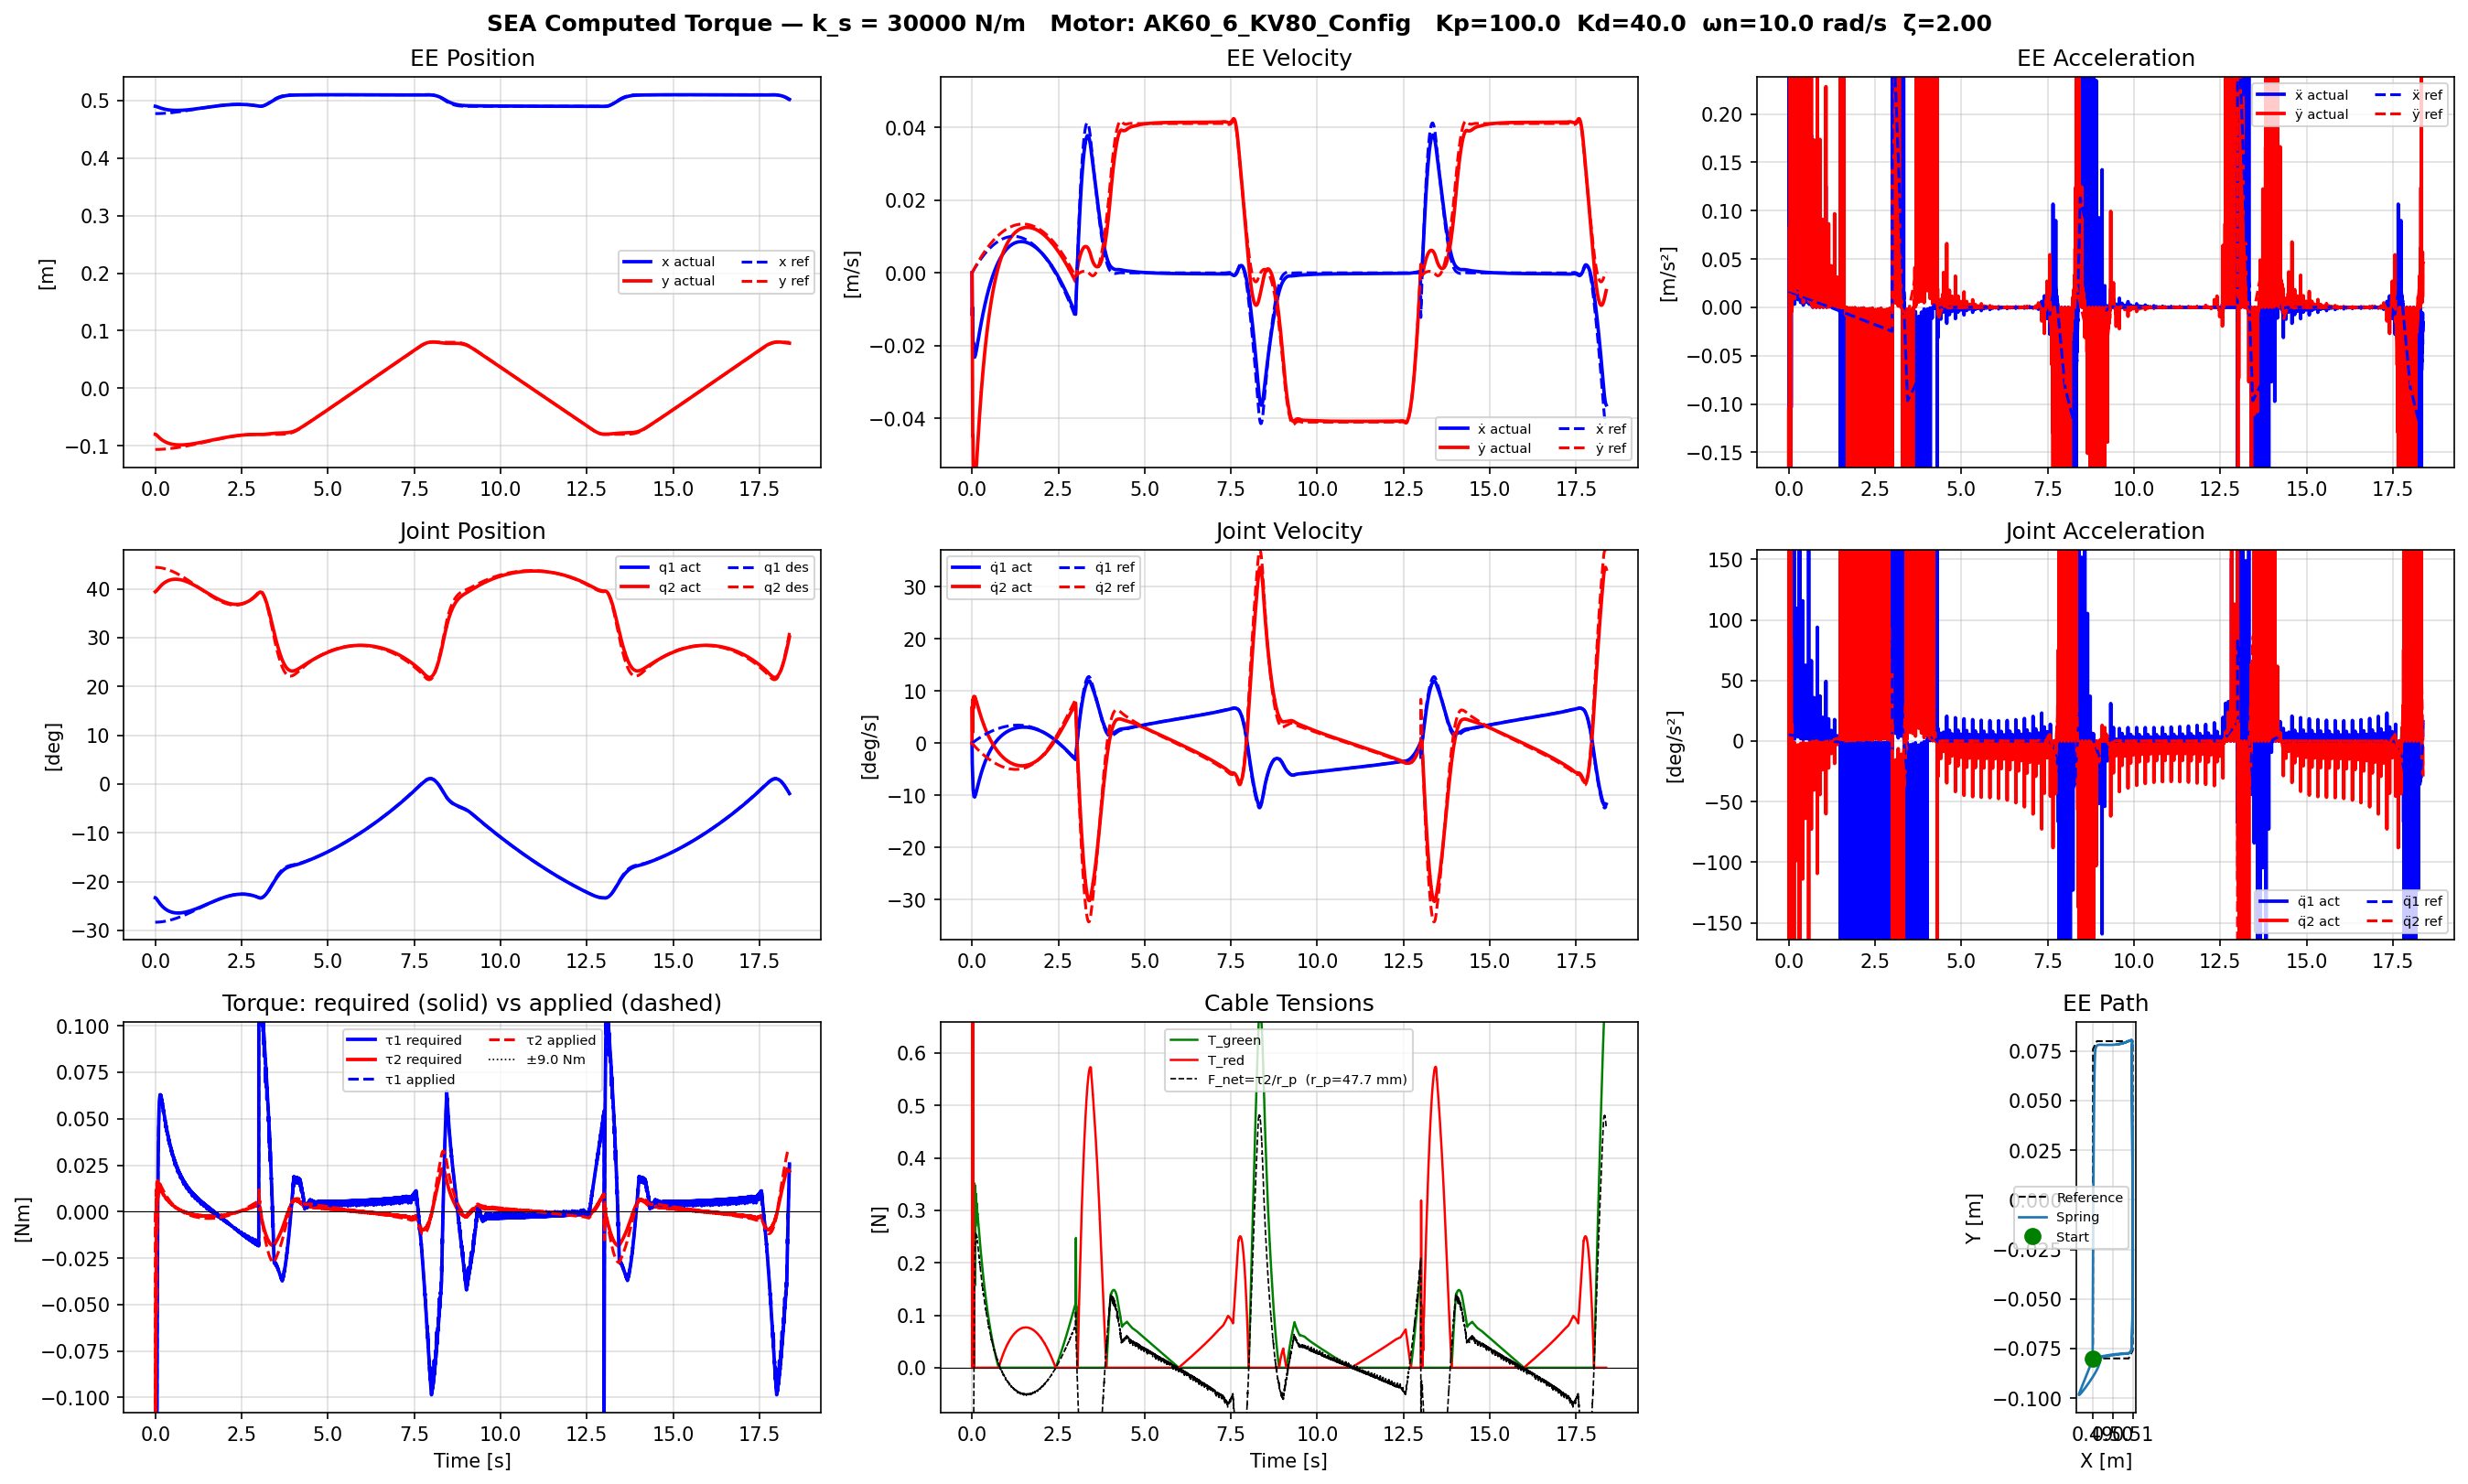
\includegraphics[width=\textwidth]{figures/sea_ct_3x3_ks30000_20260411_131829.png}
    \caption{CT 3$\times$3 performance panel at $\ks = 30\,000$\,N/m.  EE position (top-left) tracks the rectangular reference closely.  Joint positions (middle-left) follow desired values with minimal lag.  Applied torque (bottom-left, dashed) almost perfectly overlays desired torque---the spring is stiff enough that $\delta_{\mathrm{ss}} = \tau_2 / (\ks \rp) \approx 0$ and the SEA acts as a rigid passthrough.  Cable tensions alternate between green and red at rectangle corners as the torque direction reverses.  The EE path (bottom-right) tightly follows the reference rectangle.}
    \label{fig:ct_ks30000}
\end{figure}

\begin{figure}[H]
    \centering
    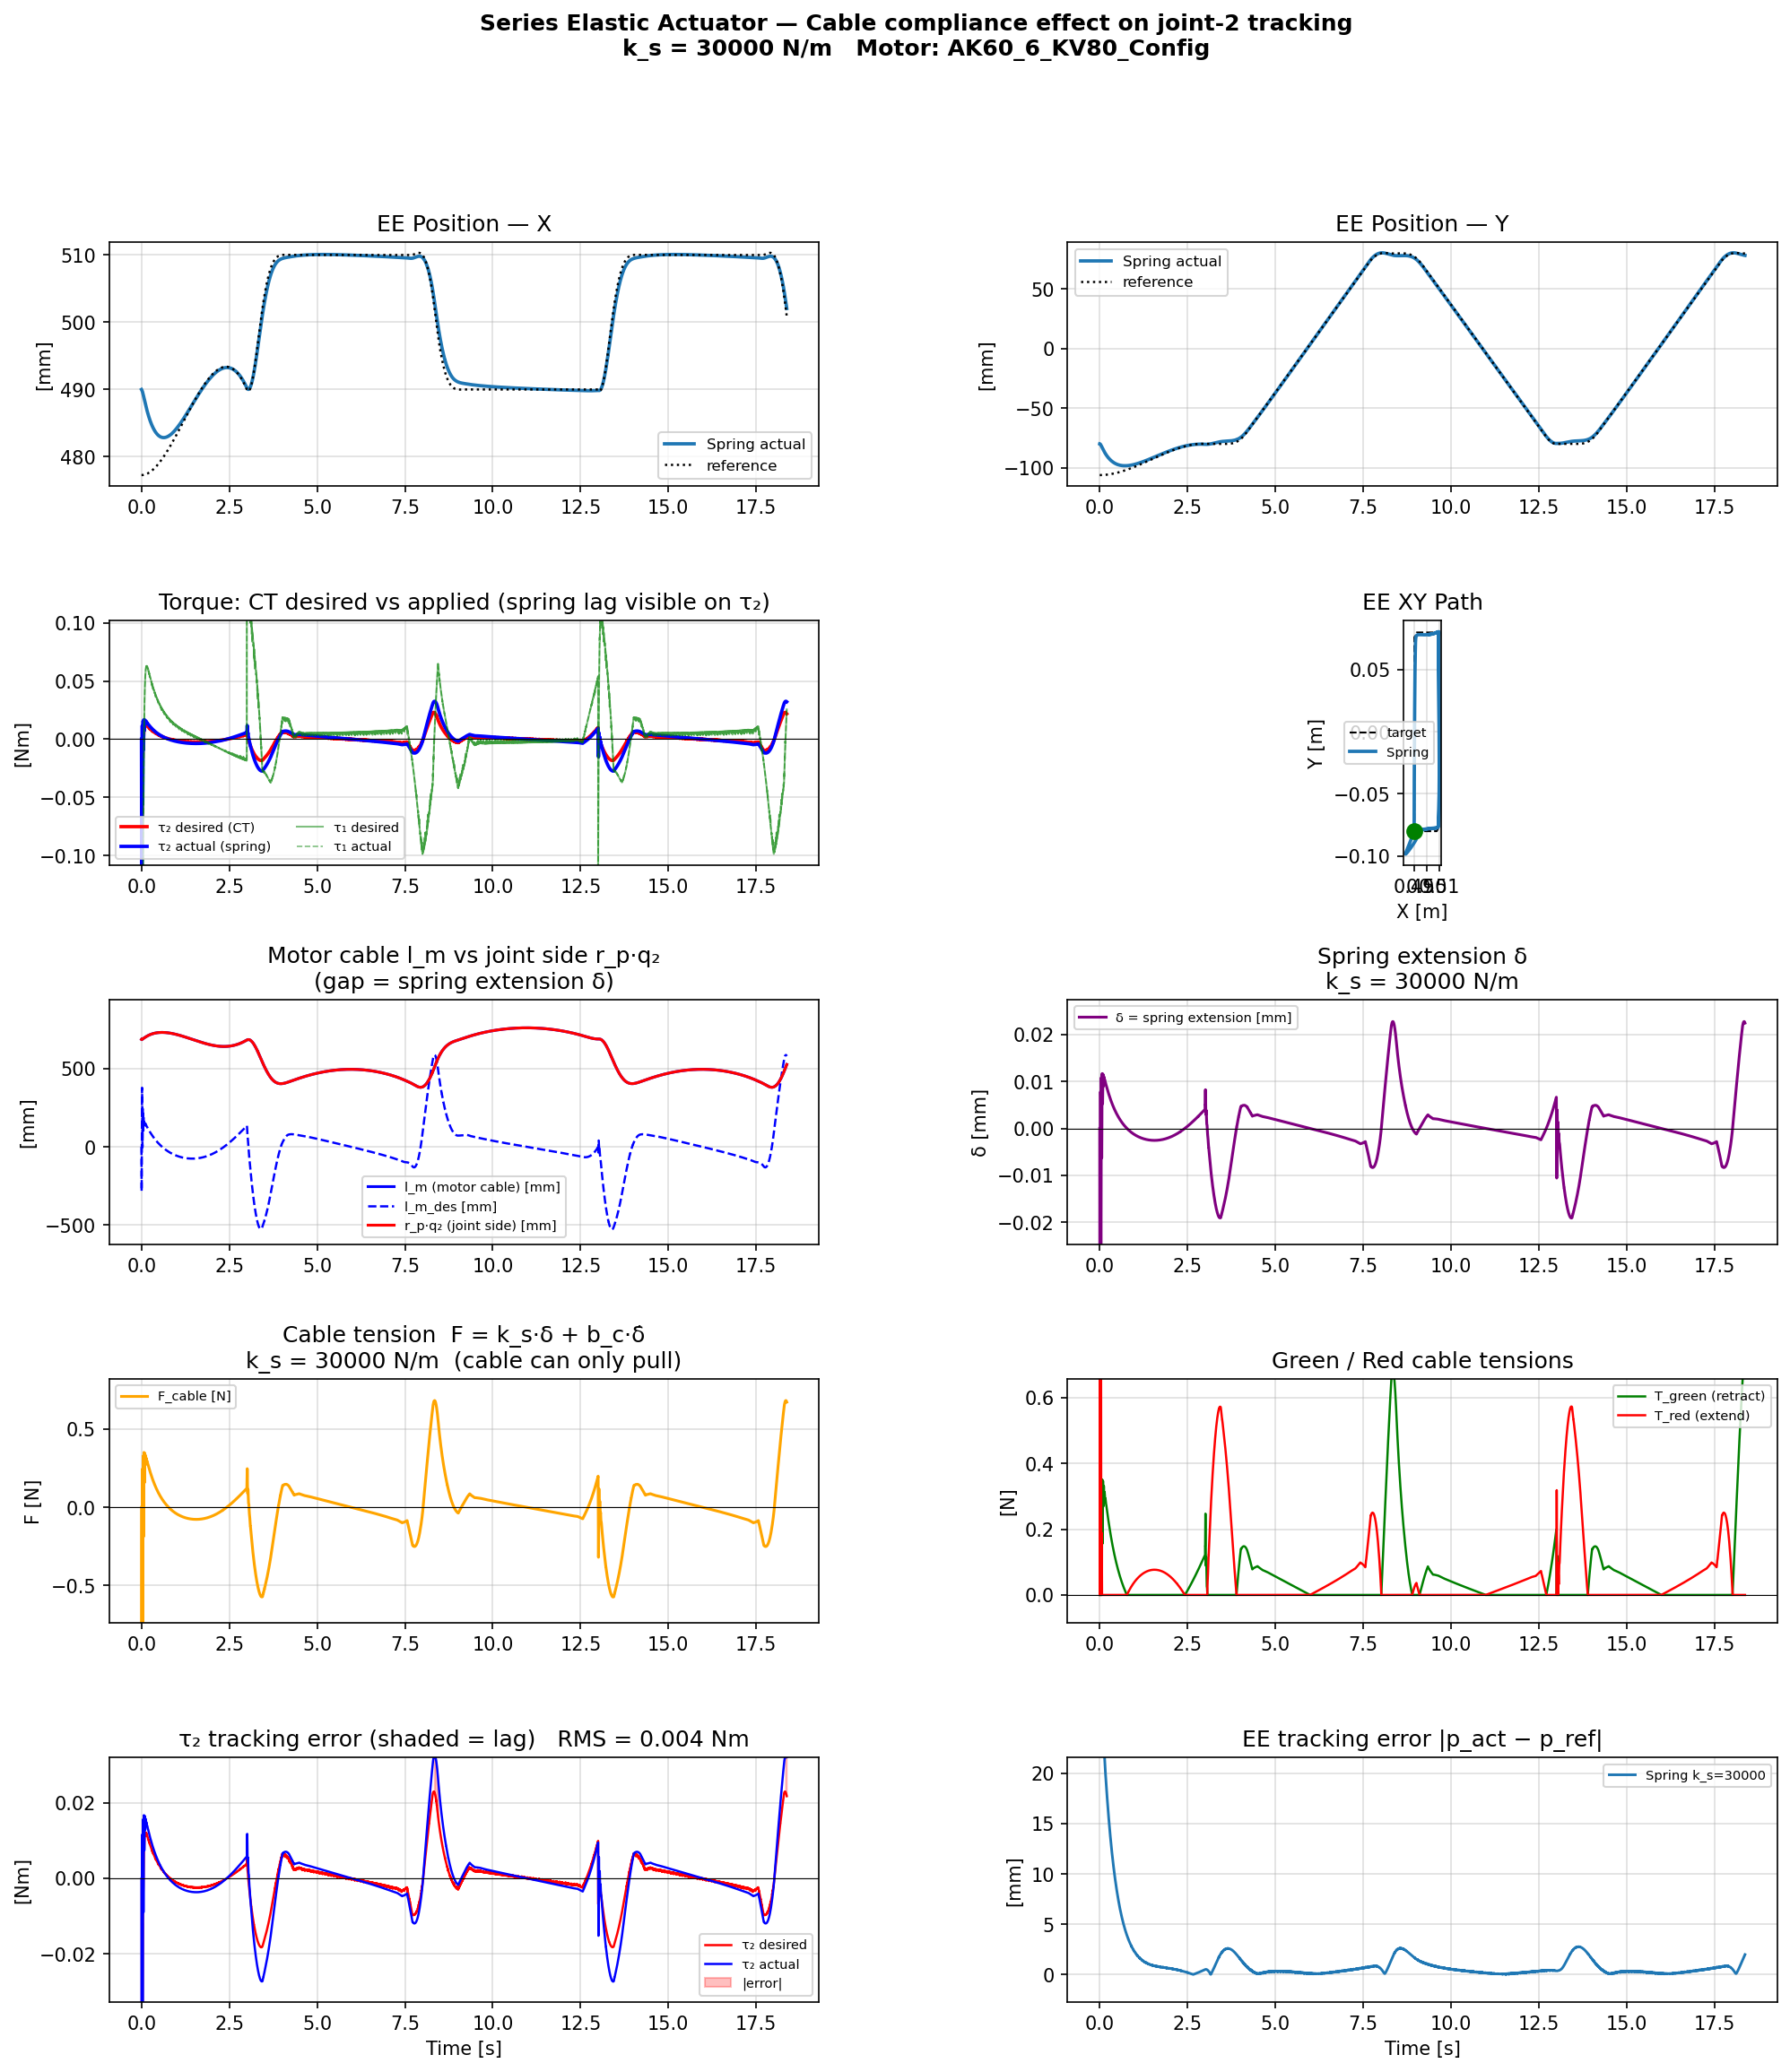
\includegraphics[width=\textwidth]{figures/sea_cable_ks30000_20260411_131829.png}
    \caption{SEA 5$\times$2 diagnostics at $\ks = 30\,000$\,N/m.  Spring extension $\delta$ (row~2, right) peaks at $\pm 0.02$\,mm---essentially zero.  Motor cable $\lm$ and joint-side $\rp q_2$ (row~2, left) are nearly superimposed, confirming negligible spring deflection.  Torque tracking RMS error is only 0.004\,Nm.  EE tracking error (row~4, right) is dominated by the move-to-start preamble; steady-state tracking stays below 5\,mm.}
    \label{fig:cable_ks30000}
\end{figure}


\subsection{Moderate Stiffness: $\ks = 3\,000$\,N/m}

An order of magnitude softer, the spring compliance becomes visible but tracking remains good.

\begin{figure}[H]
    \centering
    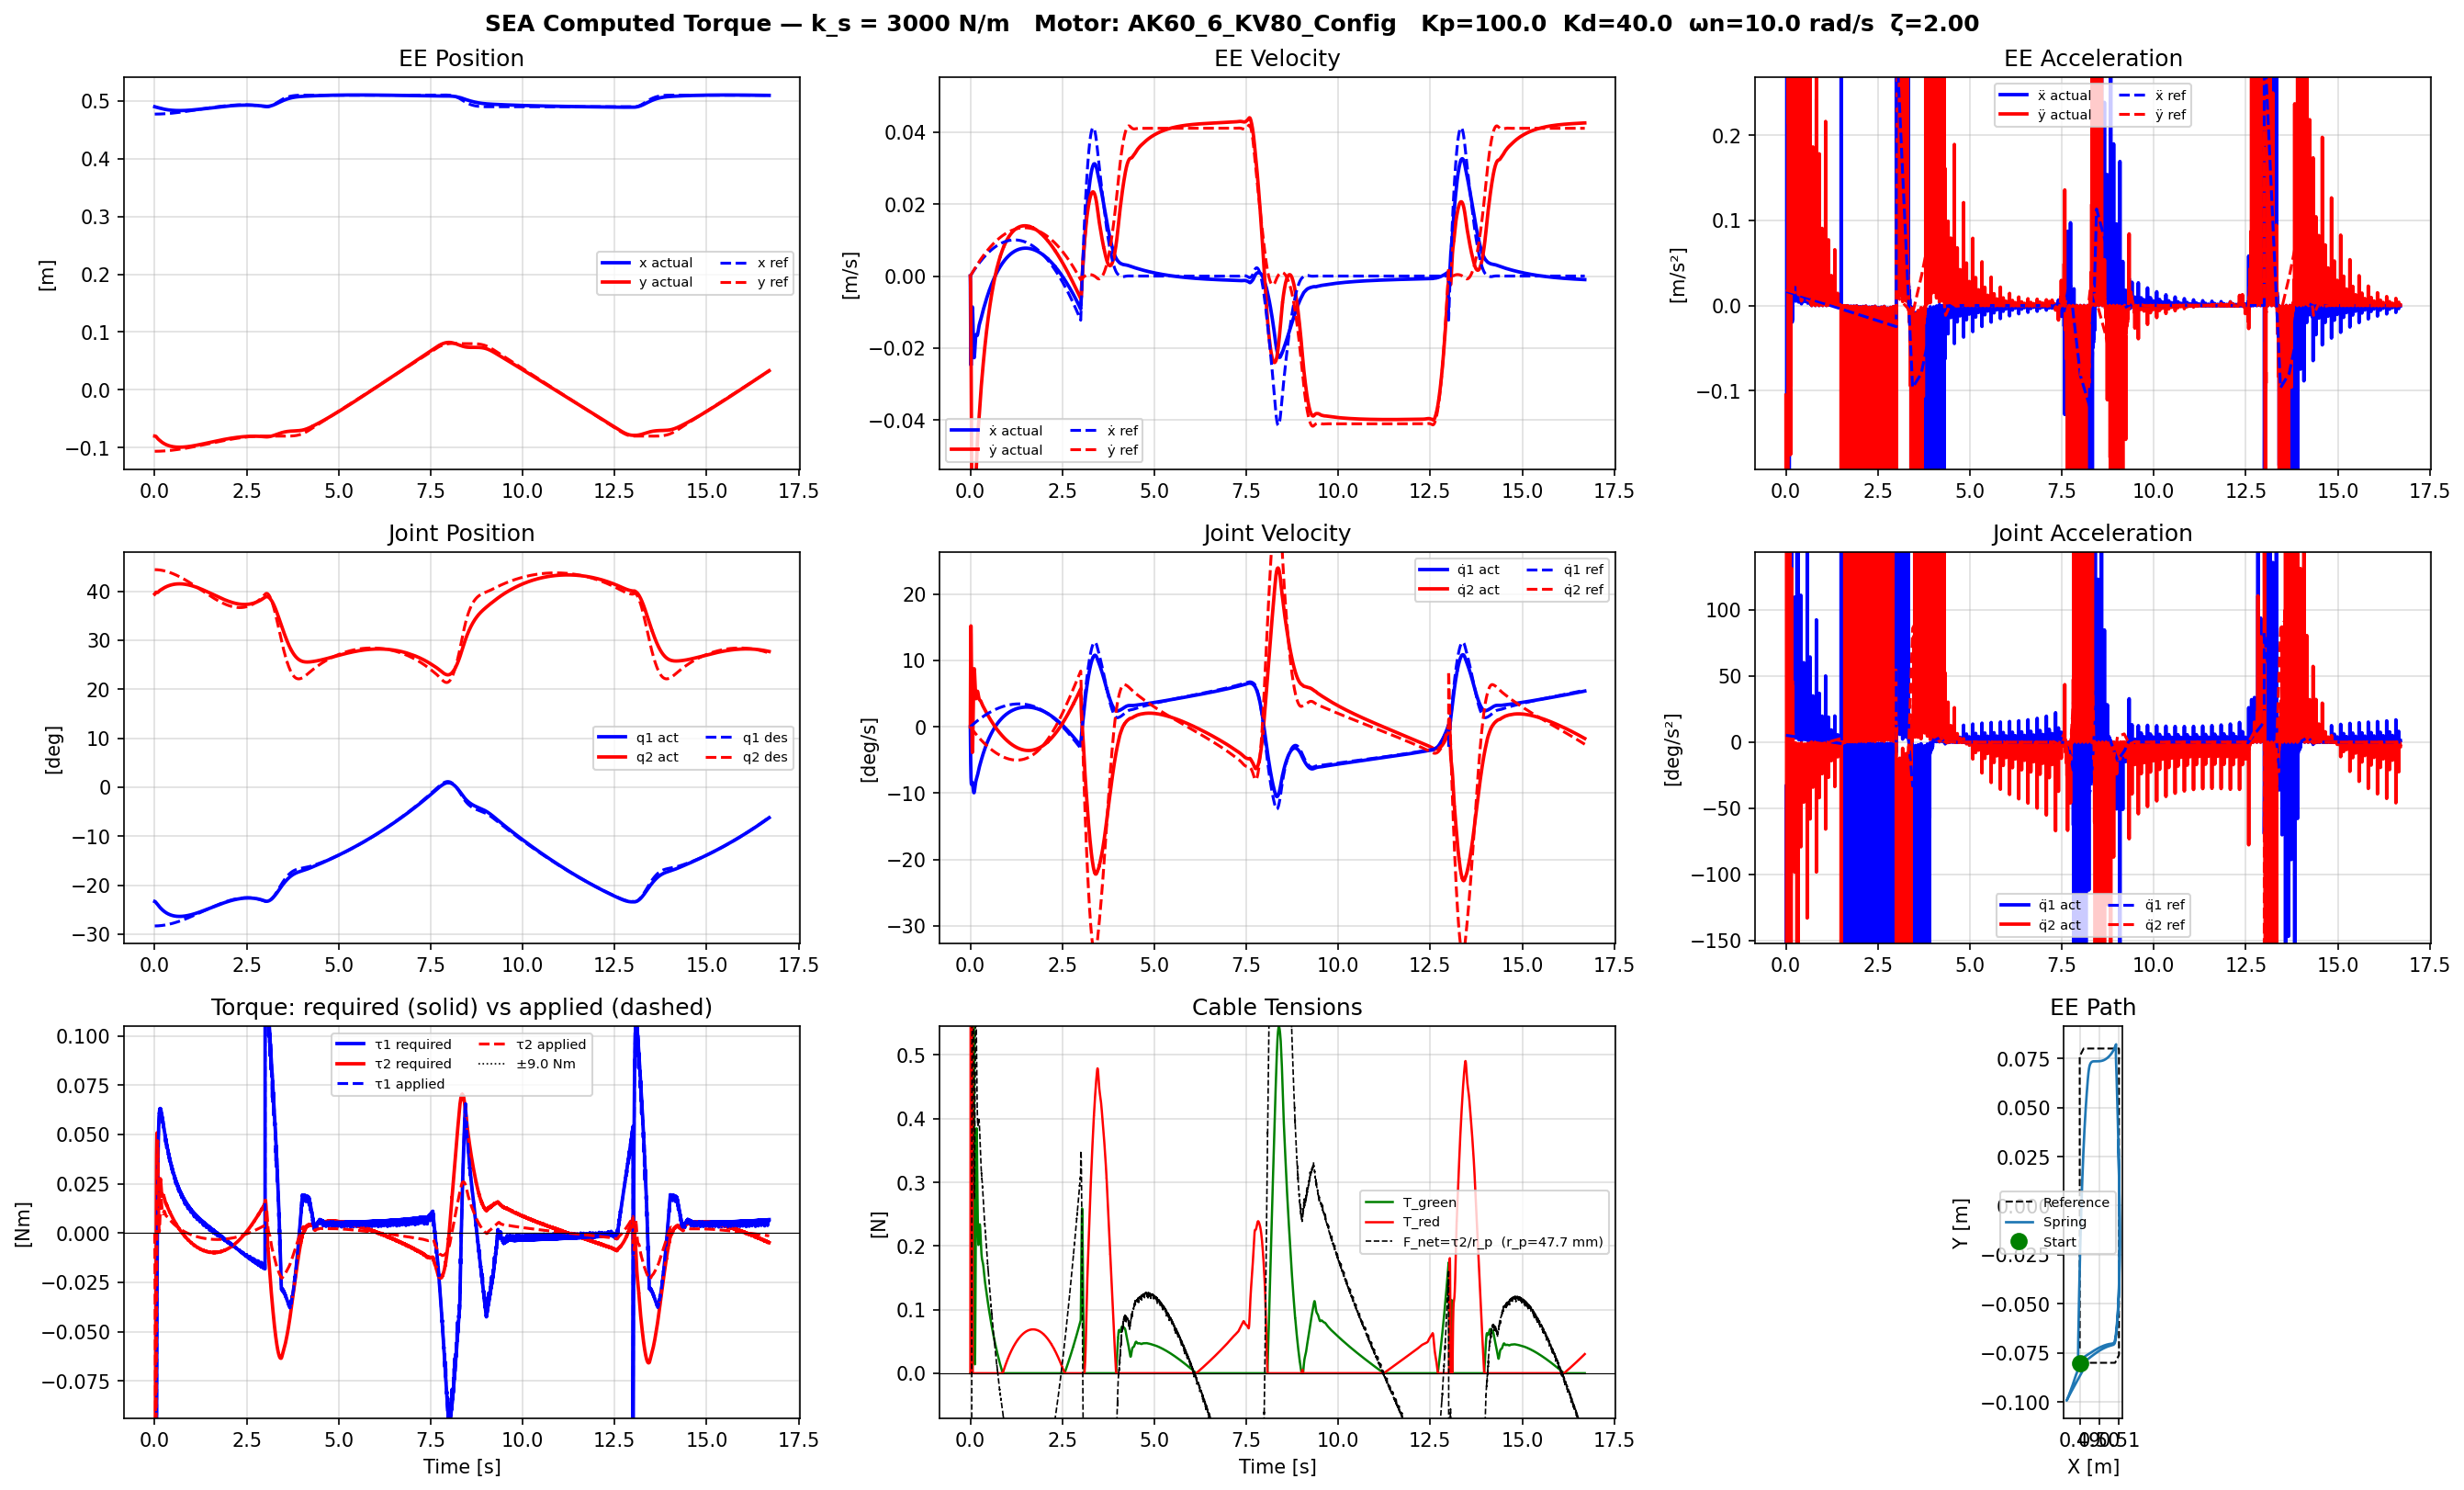
\includegraphics[width=\textwidth]{figures/sea_ct_3x3_ks3000_20260411_125341.png}
    \caption{CT 3$\times$3 performance at $\ks = 3\,000$\,N/m.  EE position tracking remains close to the reference.  Velocity and acceleration show slight deviations at rectangle corners.  Applied torque $\tau_2$ (bottom-left, dashed) follows desired torque closely but with a visible phase lag at transients---the spring cannot respond instantaneously.  Cable tensions peak at $\approx 0.5$\,N during the sharp direction changes.}
    \label{fig:ct_ks3000}
\end{figure}

\begin{figure}[H]
    \centering
    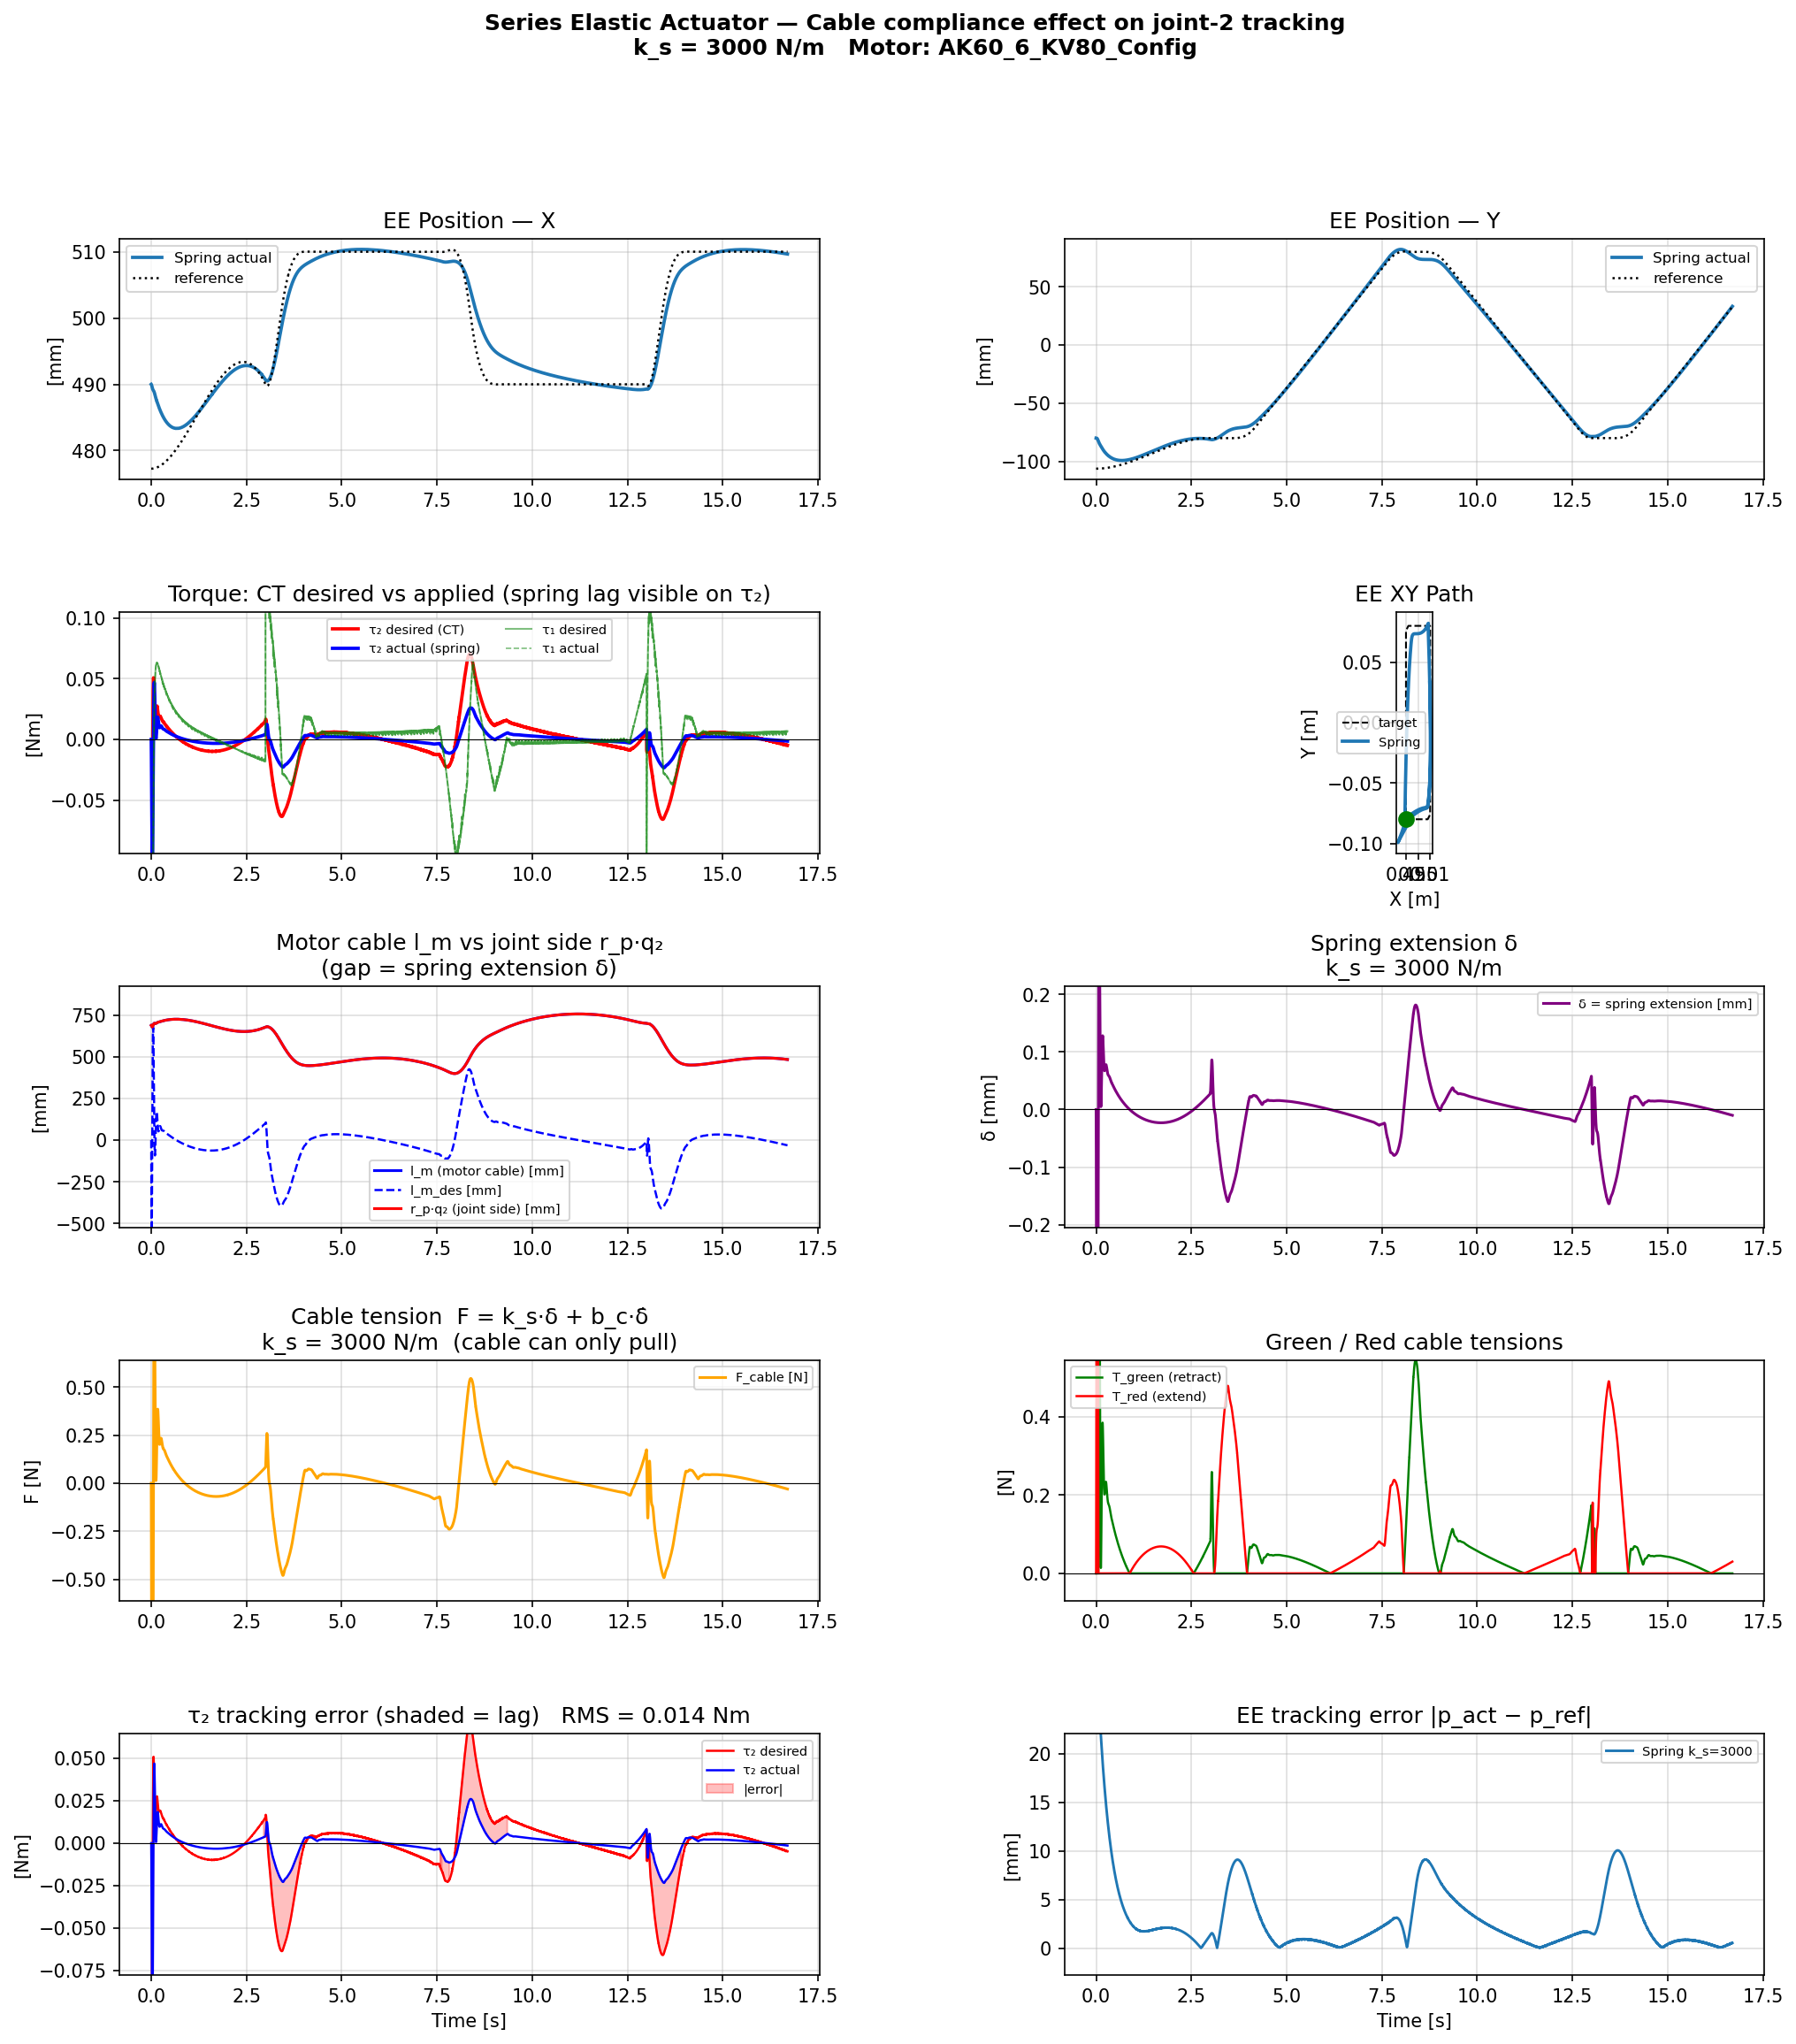
\includegraphics[width=\textwidth]{figures/sea_cable_ks3000_20260411_125341.png}
    \caption{SEA diagnostics at $\ks = 3\,000$\,N/m.  Spring extension $\delta$ (row~2, right) now reaches $\pm 0.2$\,mm---an order of magnitude larger than $\ks = 30\,000$.  The gap between $\lm$ and $\rp q_2$ (row~2, left) is visible but small.  Torque tracking RMS error is 0.014\,Nm, $3.5\times$ worse than the near-rigid case.  EE tracking error remains below $\approx 20$\,mm, with peaks at corners where the spring cannot follow the sudden torque demand.}
    \label{fig:cable_ks3000}
\end{figure}


\subsection{Compliant: $\ks = 300$\,N/m}

At this stiffness the spring lag becomes the dominant error source.

\begin{figure}[H]
    \centering
    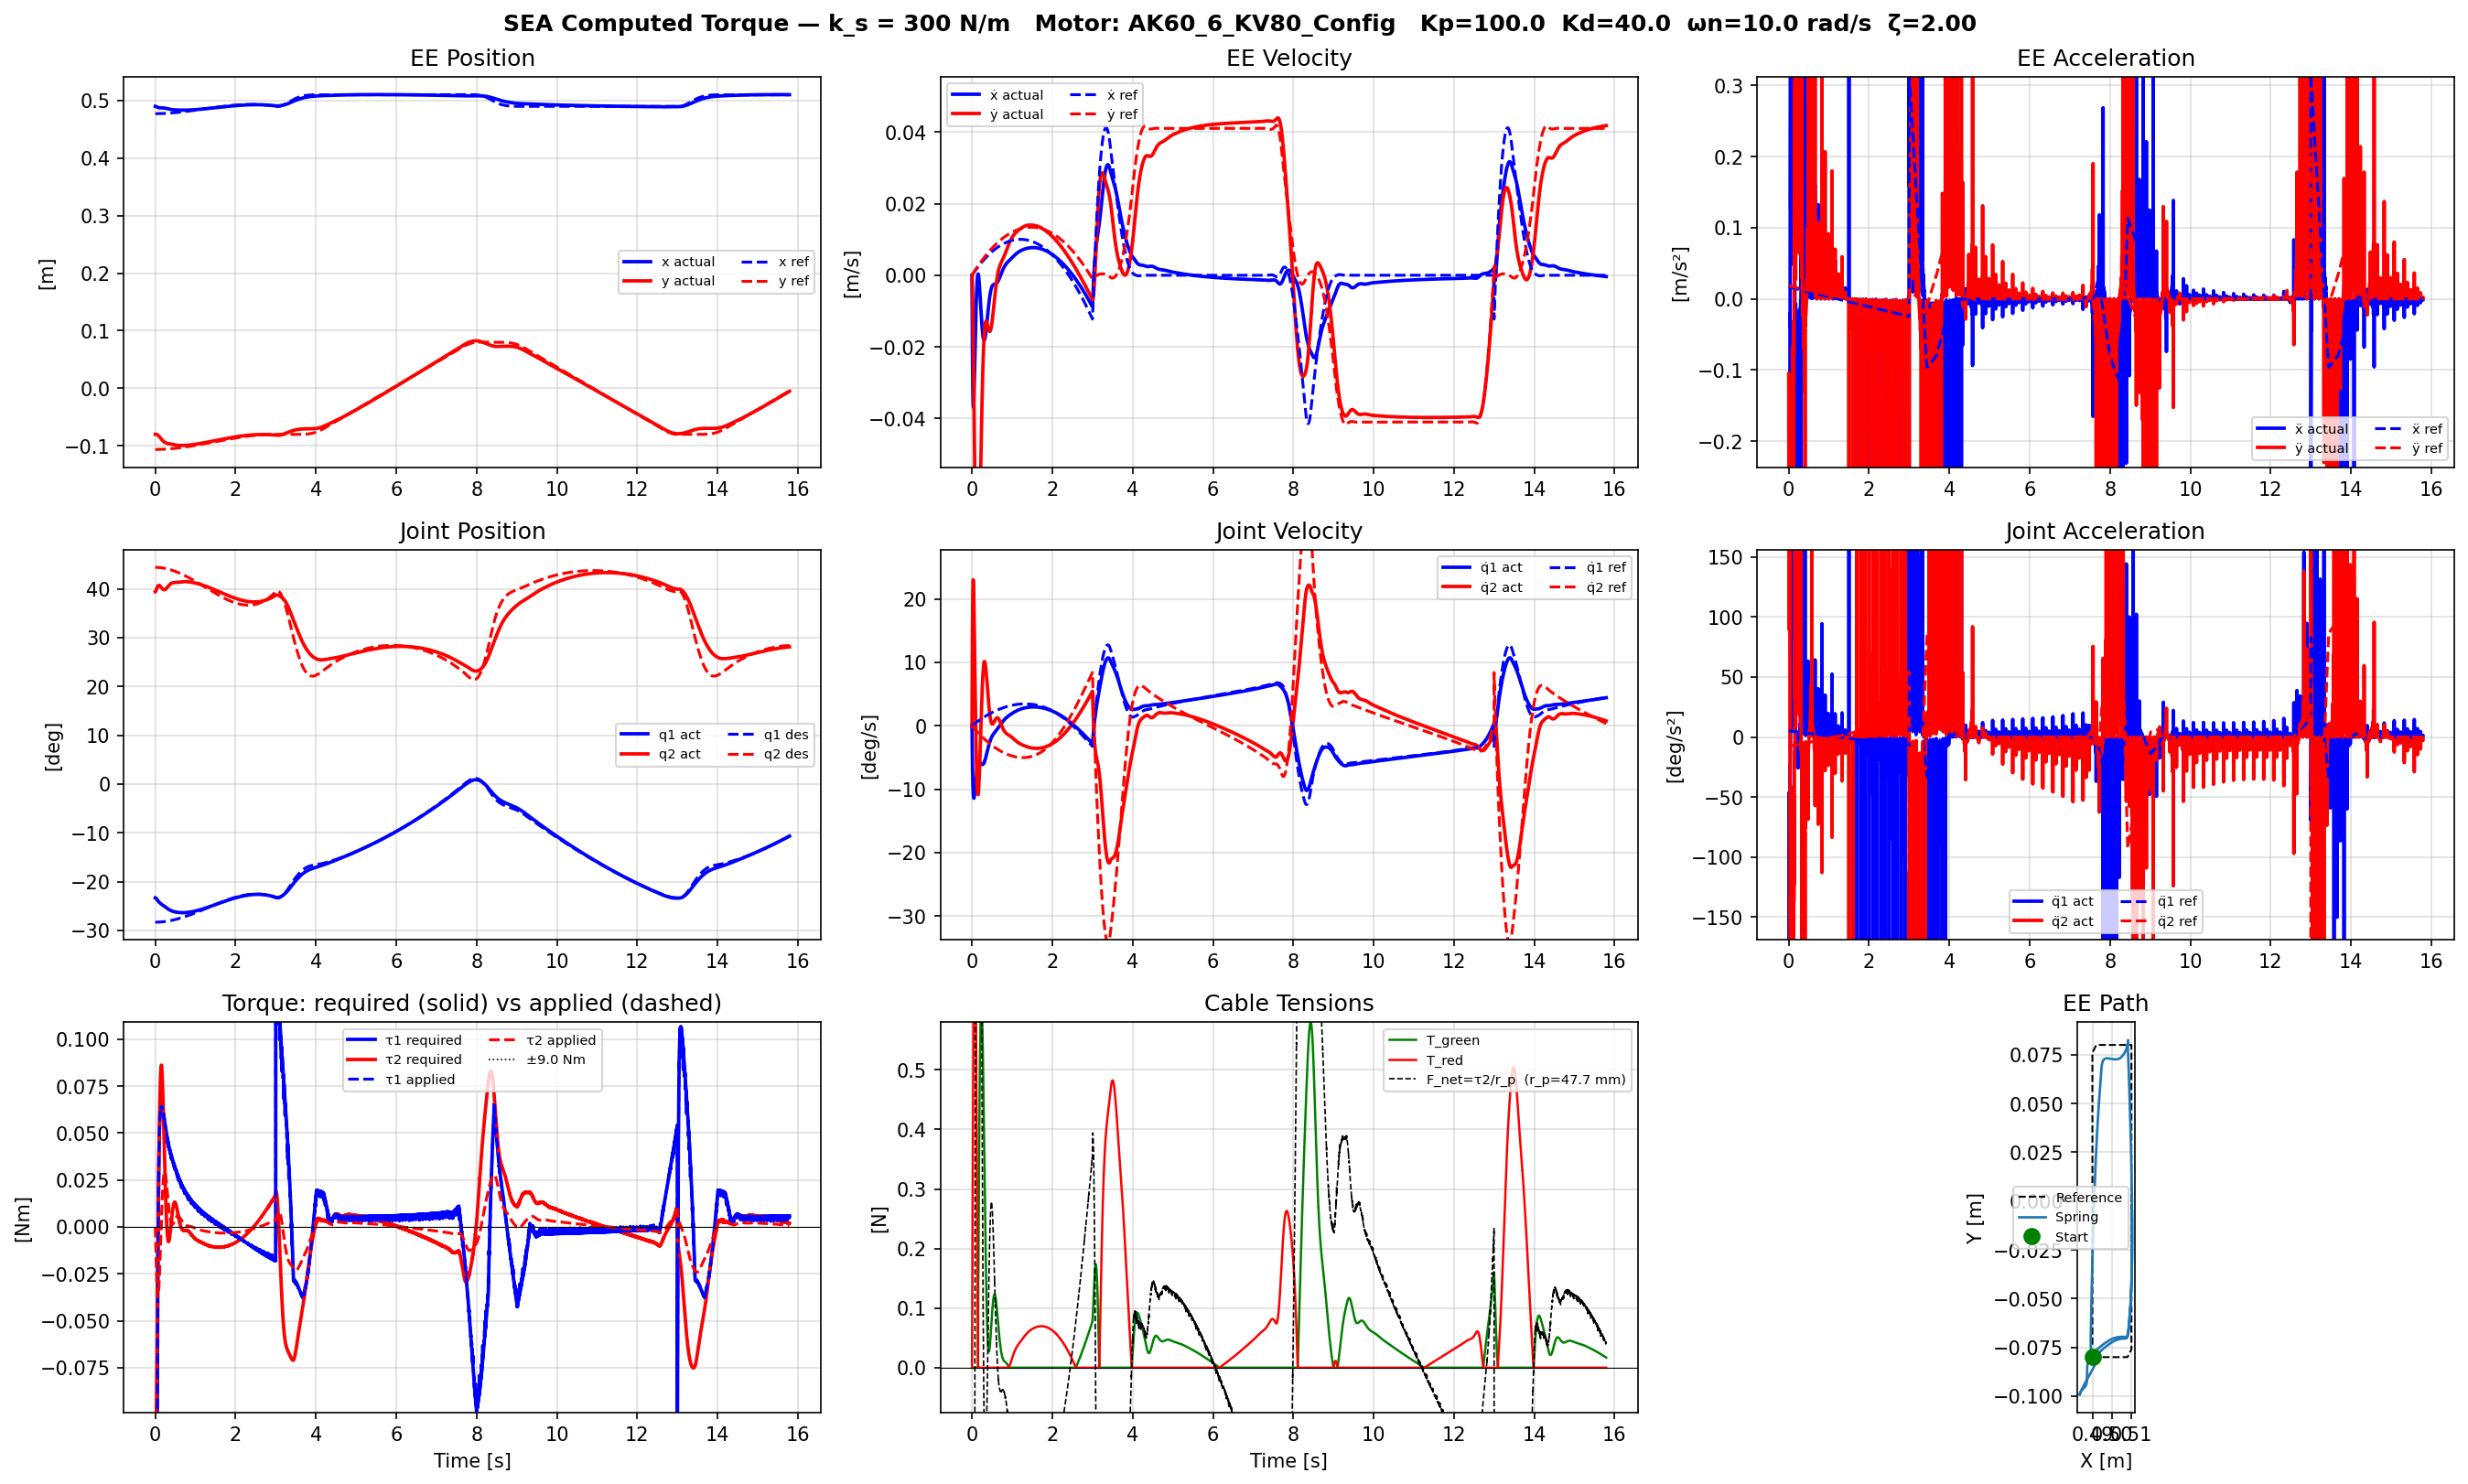
\includegraphics[width=\textwidth]{figures/sea_ct_3x3_ks300_20260411_125410.png}
    \caption{CT 3$\times$3 performance at $\ks = 300$\,N/m.  EE position shows noticeable deviation from reference at rectangle corners.  Joint positions (middle row) show $q_2$ actual lagging behind desired by several degrees during fast direction changes.  Applied $\tau_2$ (bottom-left) now clearly lags the desired torque with visible phase shift.  Cable tensions are smaller (peak $\approx 0.4$\,N) because the spring absorbs more energy before transmitting it.}
    \label{fig:ct_ks300}
\end{figure}

\begin{figure}[H]
    \centering
    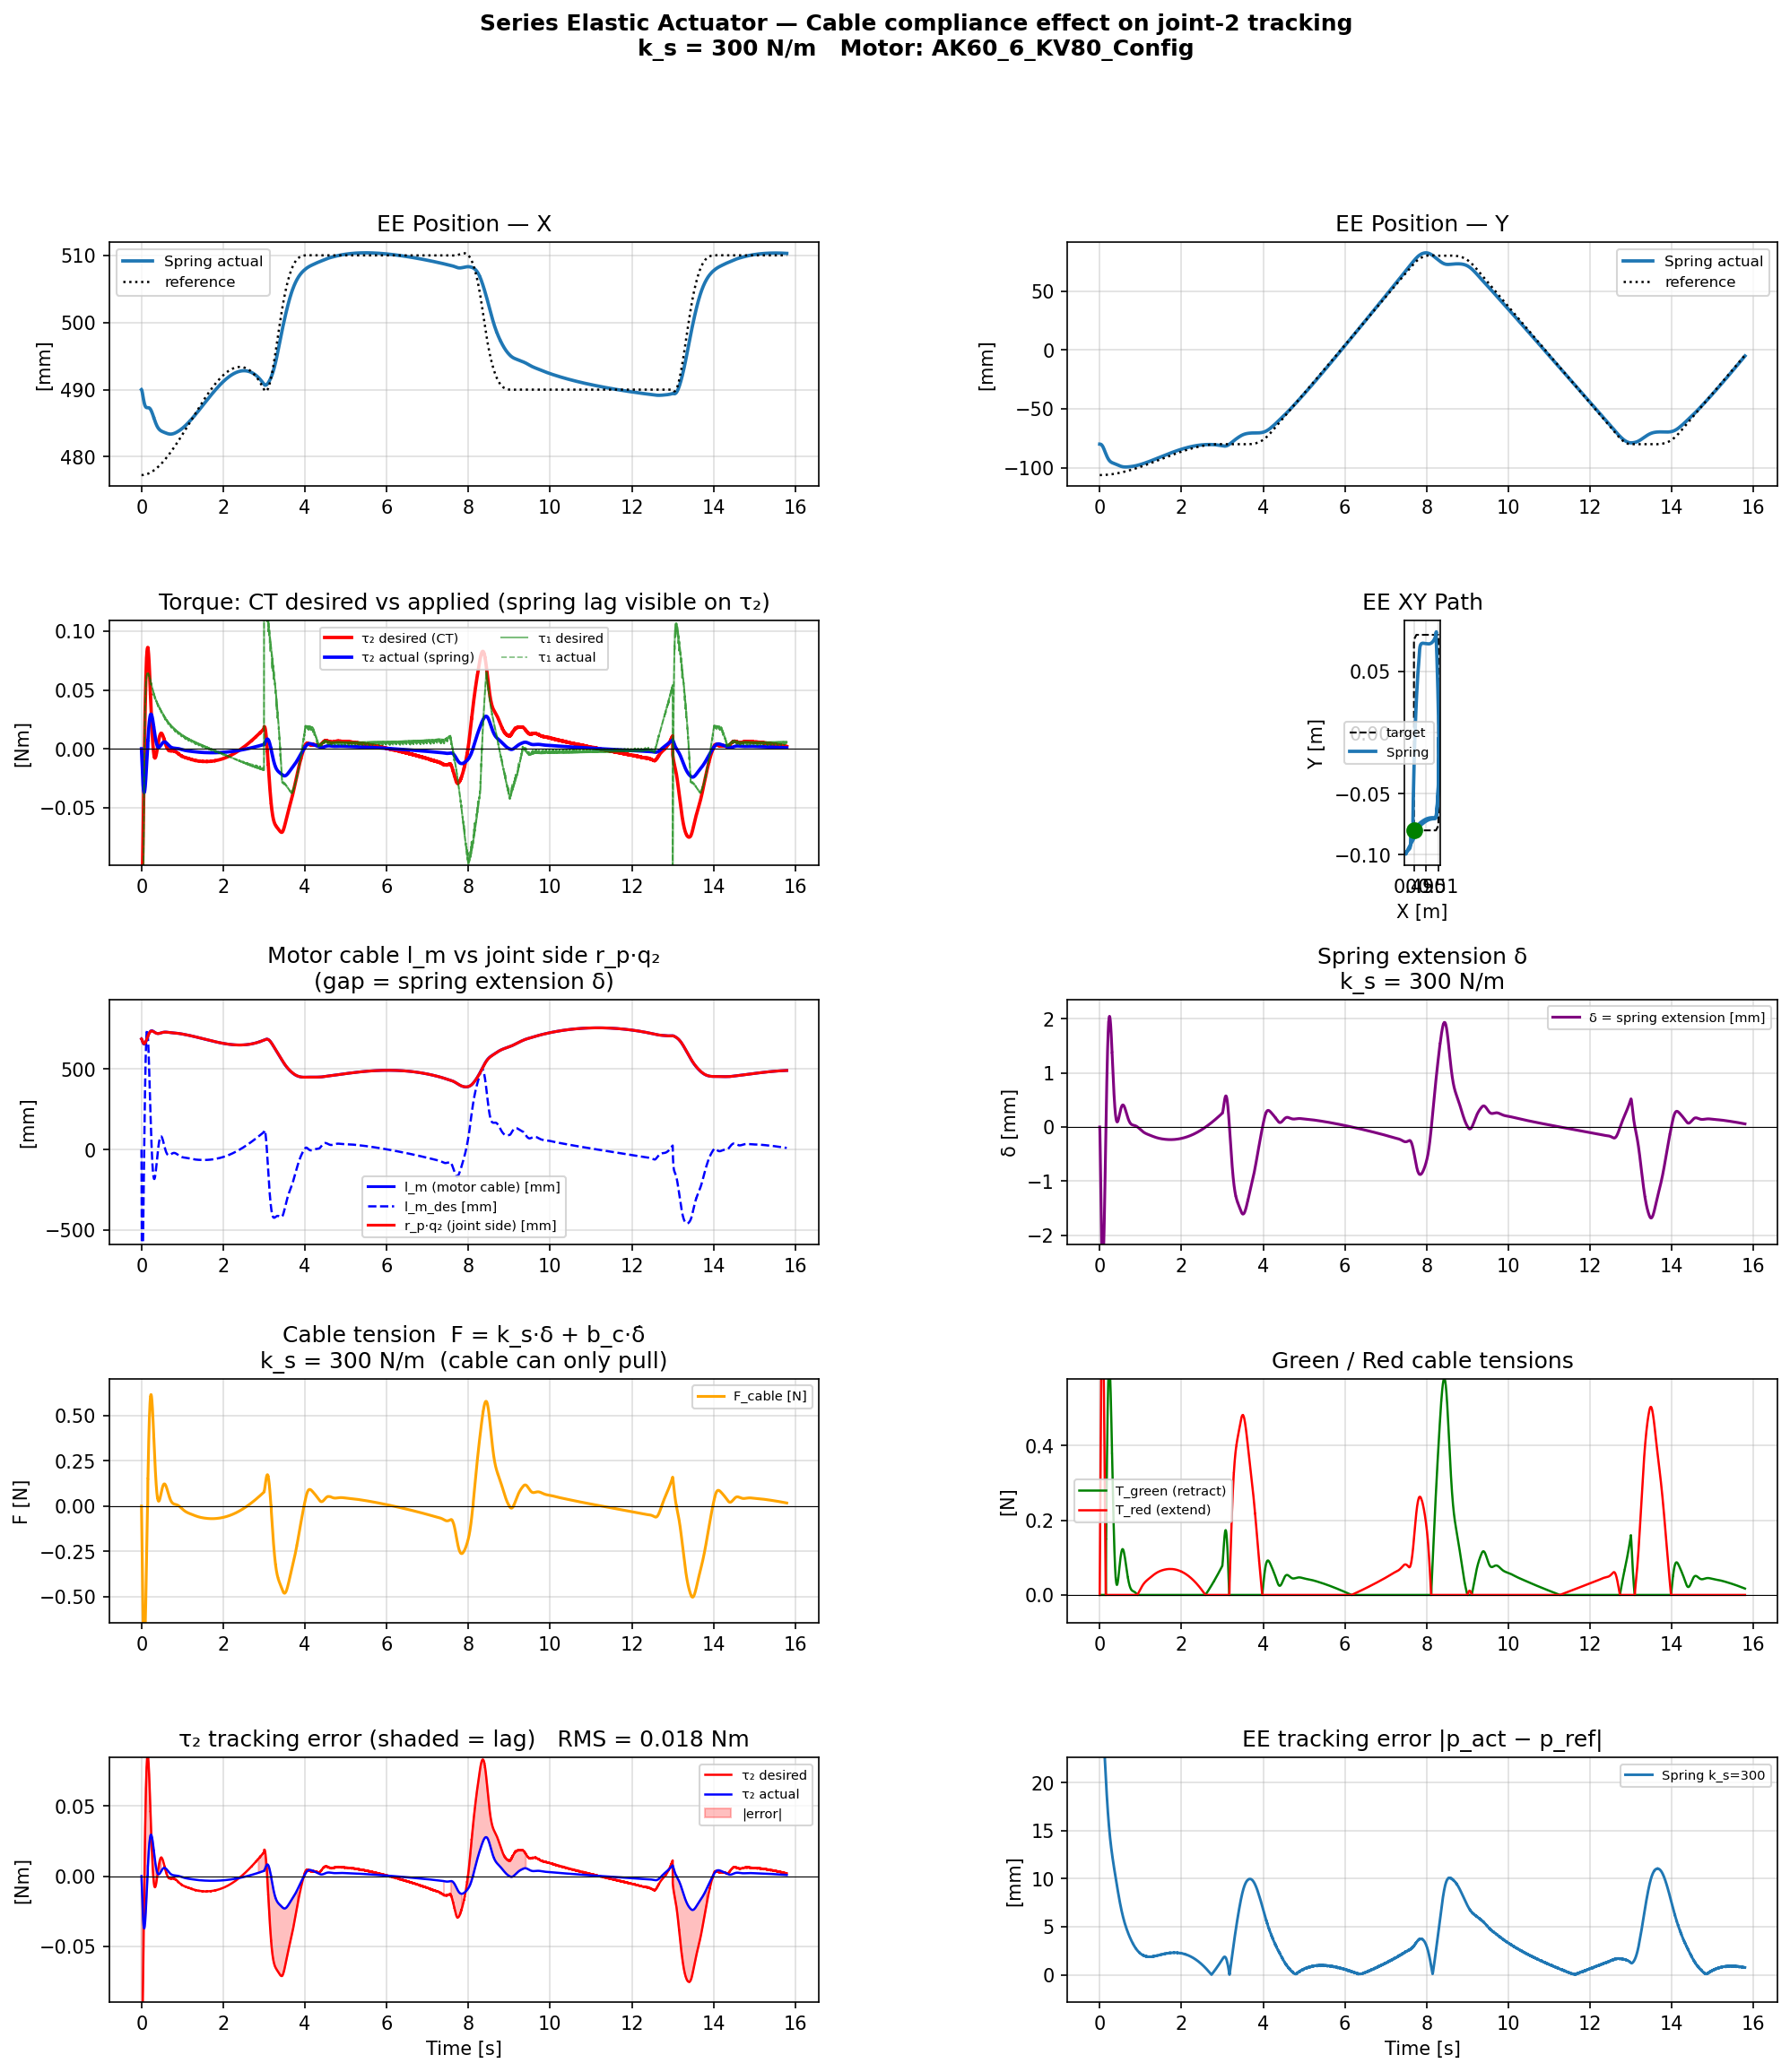
\includegraphics[width=\textwidth]{figures/sea_cable_ks300_20260411_125410.png}
    \caption{SEA diagnostics at $\ks = 300$\,N/m.  Spring extension $\delta$ (row~2, right) reaches $\pm 2$\,mm---$10\times$ larger than $\ks = 3\,000$.  The gap between $\lm$ and $\rp q_2$ (row~2, left) is now clearly visible, showing the motor leading the joint.  Torque tracking RMS error is 0.018\,Nm.  EE tracking error peaks at $\approx 20$\,mm, primarily at corners.  In torque mode, reducing $\ks$ by $10\times$ lowers the motor--spring resonance $\omega_n$ by $\sqrt{10} \approx 3.2\times$, which slows the motor response and slightly worsens torque tracking ($0.014 \to 0.018$\,Nm RMS).  However, the softer spring also reduces force per unit deflection ($F = \ks \delta$), so the overall degradation is moderate.}
    \label{fig:cable_ks300}
\end{figure}


\subsection{Very Soft: $\ks = 30$\,N/m}

At this extreme, the spring dominates the entire system response.

\begin{figure}[H]
    \centering
    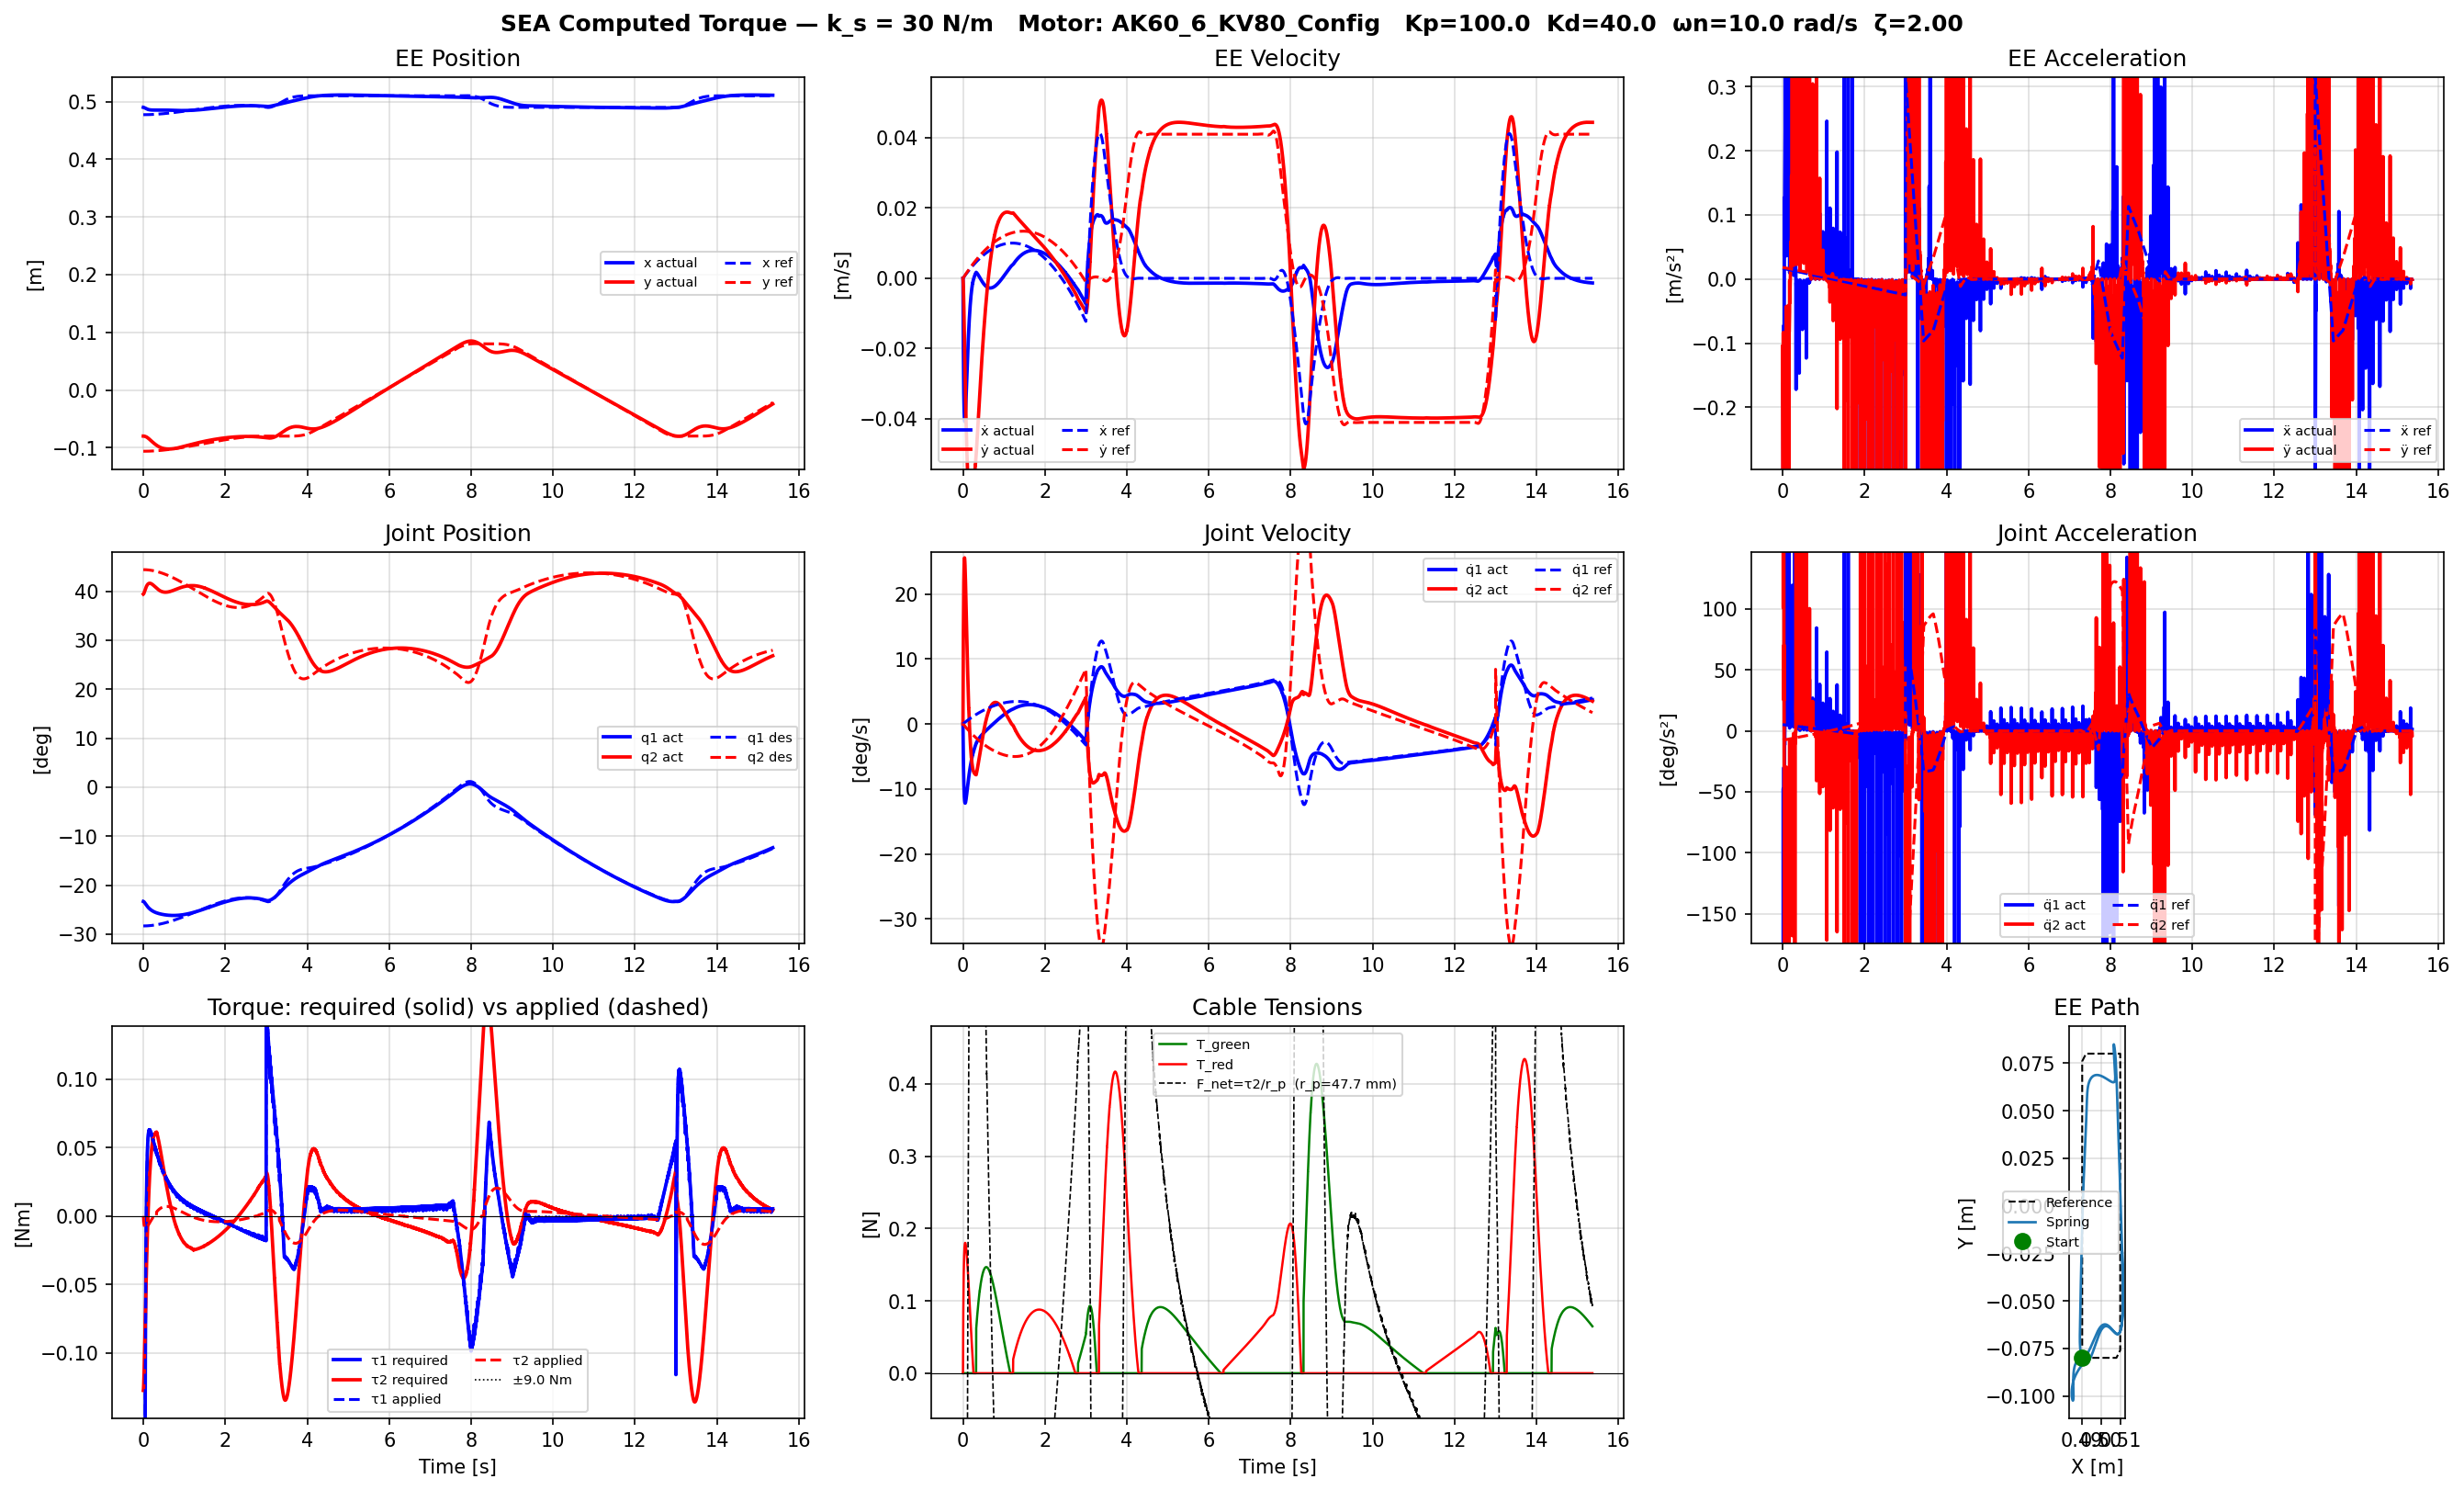
\includegraphics[width=\textwidth]{figures/sea_ct_3x3_ks30_20260411_125524.png}
    \caption{CT 3$\times$3 performance at $\ks = 30$\,N/m.  EE position (top row) shows significant deviation from reference---the arm overshoots corners and lags on straight segments.  Joint-2 position (middle-left, red) deviates substantially from desired (dashed), with the joint settling slowly after each direction change.  Applied $\tau_2$ is heavily filtered by the soft spring, with large phase lag.  The EE path (bottom-right) departs noticeably from the rectangle, cutting corners and exhibiting hysteresis.}
    \label{fig:ct_ks30}
\end{figure}

\begin{figure}[H]
    \centering
    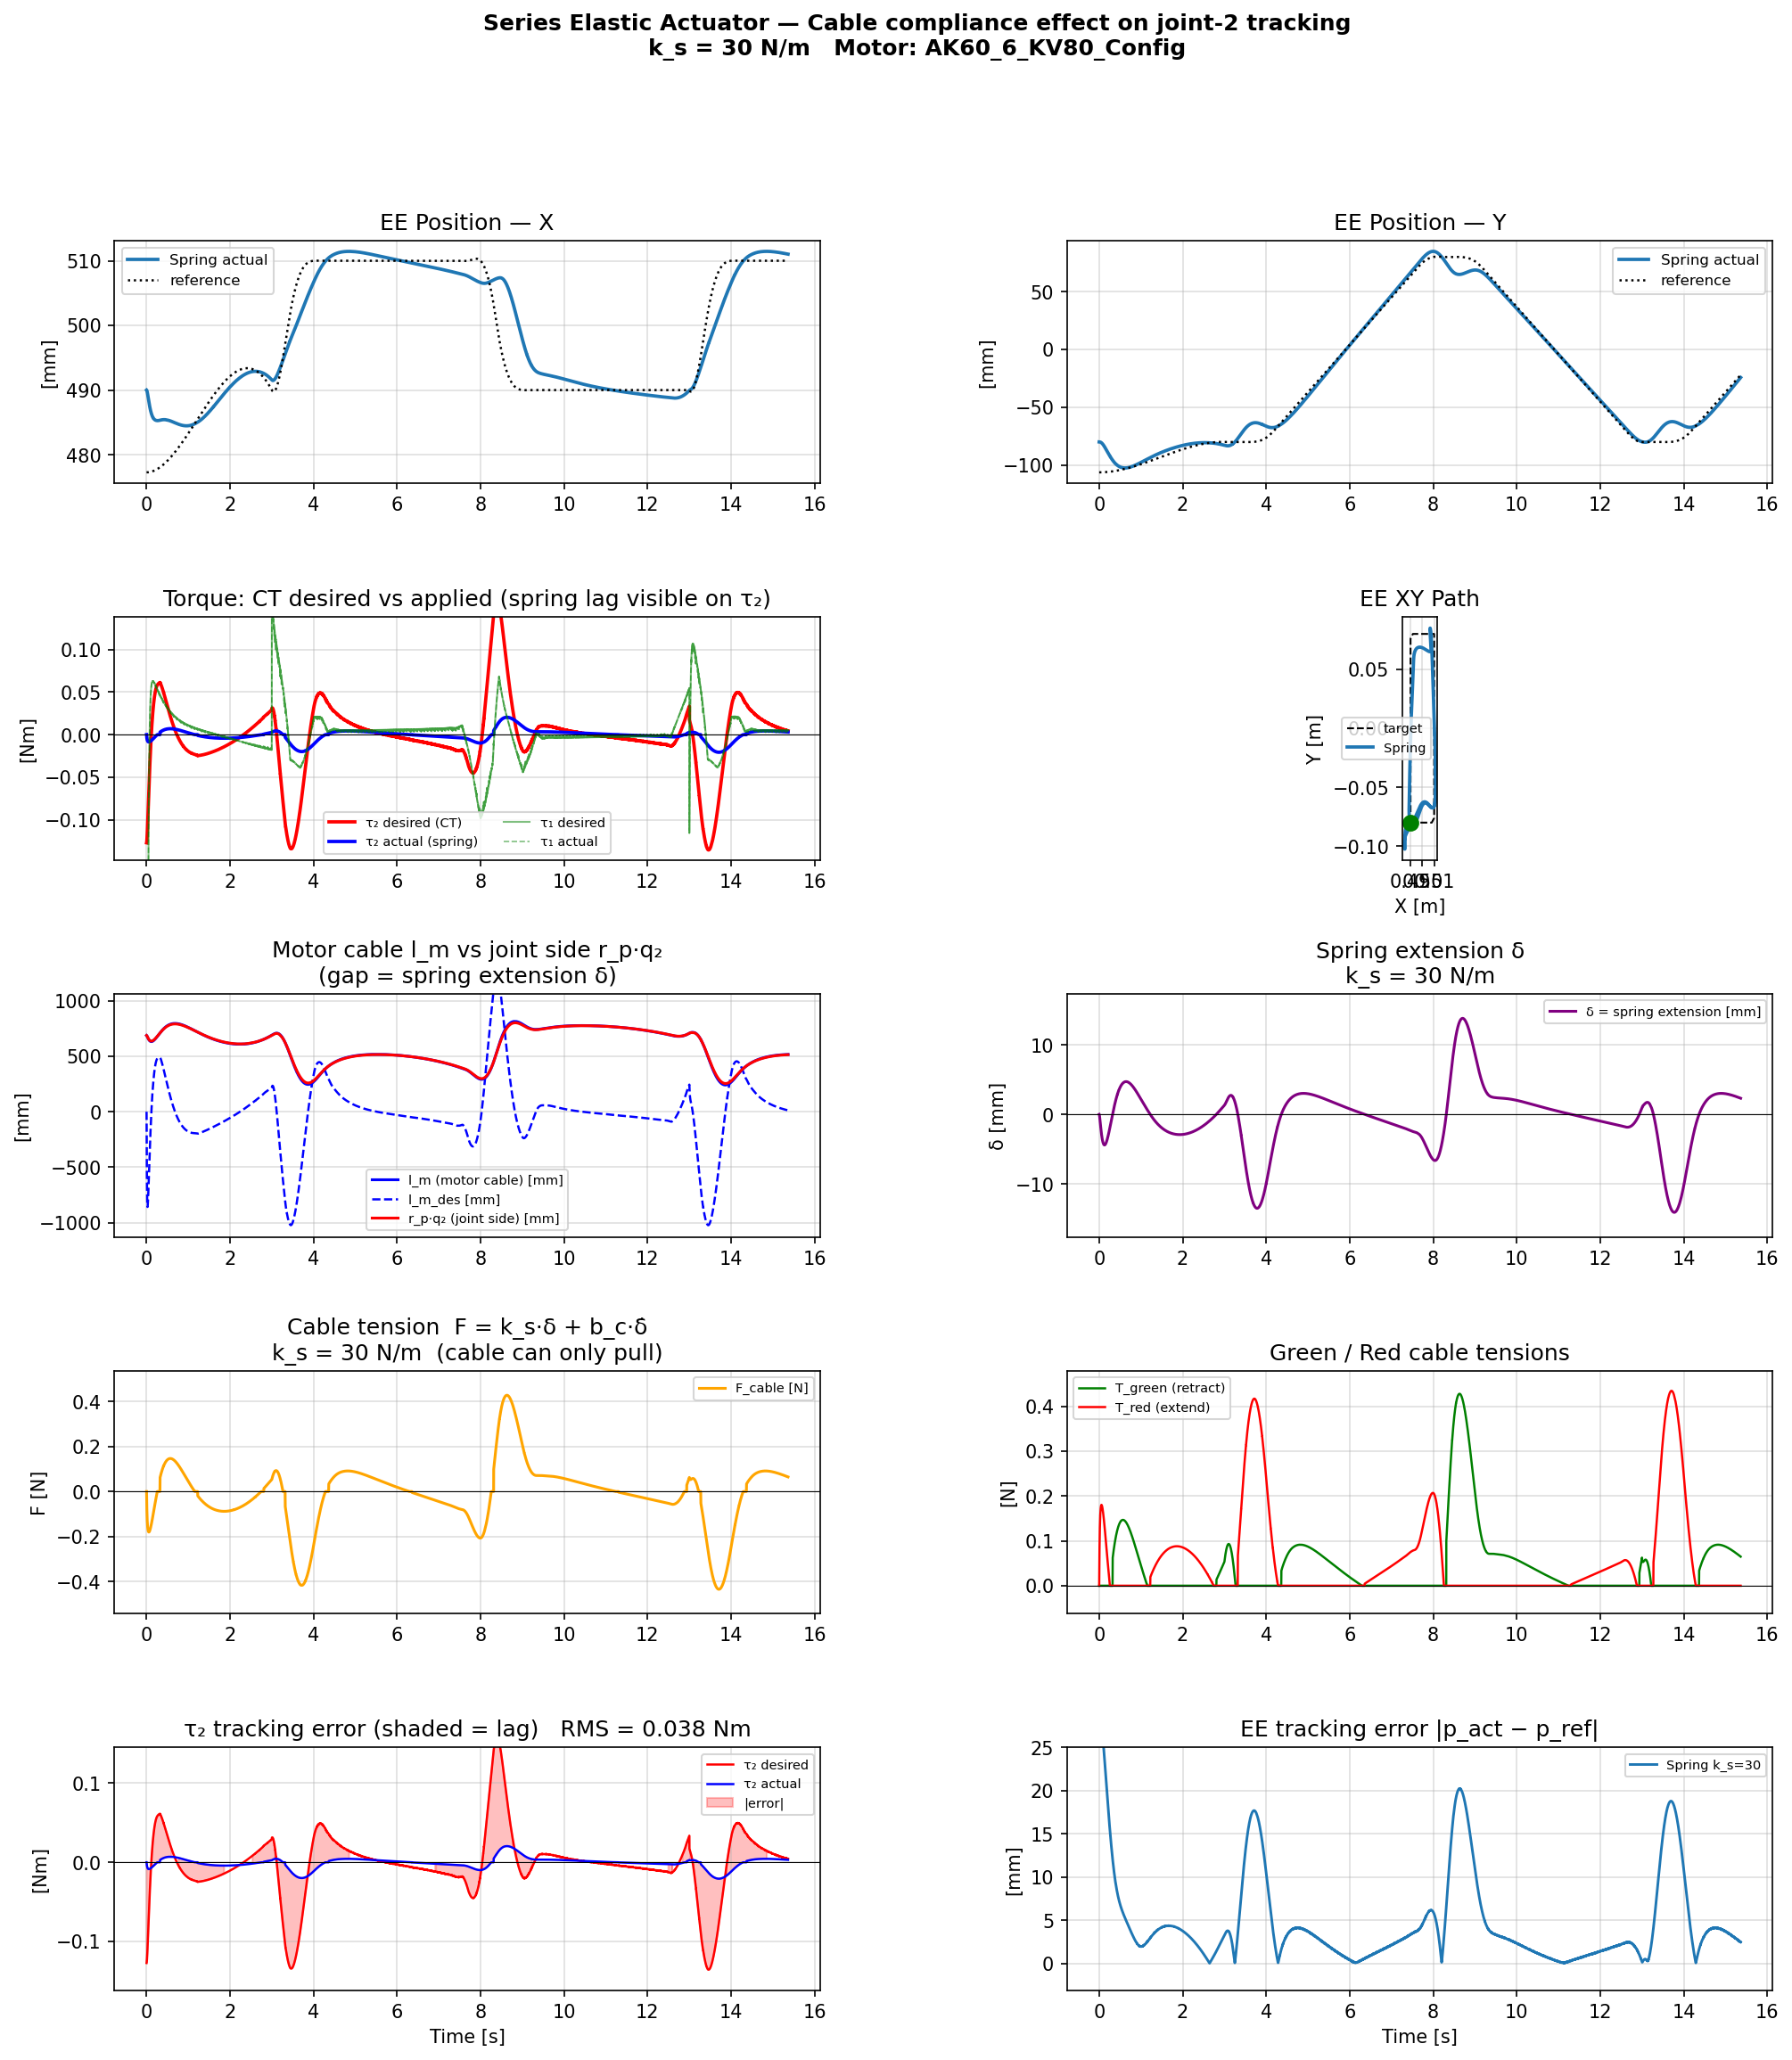
\includegraphics[width=\textwidth]{figures/sea_cable_ks30_20260411_125524.png}
    \caption{SEA diagnostics at $\ks = 30$\,N/m.  Spring extension $\delta$ (row~2, right) reaches $\pm 15$\,mm---nearly $1000\times$ the near-rigid case.  Motor cable $\lm$ and joint side $\rp q_2$ (row~2, left) diverge dramatically: the motor must travel far ahead of the joint to stretch the soft spring enough to produce the required force.  Torque tracking RMS error is 0.038\,Nm ($10\times$ worse than near-rigid).  EE tracking peaks at $\approx 25$\,mm.  The cable force (row~3) is smaller in magnitude because $F = \ks \delta$ with small $\ks$, even though $\delta$ is large.}
    \label{fig:cable_ks30}
\end{figure}


\subsection{Stiffness Sweep Summary}

\begin{table}[H]
\centering
\caption{Effect of spring stiffness on tracking quality (torque mode, CubeMars AK60-6).}
\label{tab:stiffness_sweep}
\begin{tabular}{rcccc}
\toprule
$\ks$ [N/m] & $\delta_{\mathrm{peak}}$ [mm] & $\tau_2$ RMS error [Nm] & EE error peak [mm] & Behaviour \\
\midrule
30\,000 & 0.02   & 0.004 & $<5$  & Near-rigid, minimal lag \\
3\,000  & 0.2    & 0.014 & $\sim$20 & Slight lag at corners \\
300     & 2      & 0.018 & $\sim$20 & Visible torque lag, larger $\delta$ \\
30      & 15     & 0.038 & $\sim$25 & Heavy lag, large motor excursion \\
\bottomrule
\end{tabular}
\end{table}

\begin{resultbox}
\textbf{Key observations from the stiffness sweep:}
\begin{enumerate}[leftmargin=2em]
    \item \textbf{Spring extension scales as $1/\ks$}: $\delta_{\mathrm{ss}} = \tau / (\ks \rp)$, so halving $\ks$ doubles the motor excursion needed.
    \item \textbf{Torque RMS error scales sublinearly with $\ks$}: Reducing $\ks$ by $1000\times$ (30\,000 $\to$ 30) only increases torque error by $\sim 10\times$, because softer springs also produce less force per unit lag.
    \item \textbf{EE tracking is dominated by transients}: Steady-state tracking is similar across all stiffnesses; the differences appear at rectangle corners where sudden torque changes expose the spring bandwidth limit.
    \item \textbf{Motor excursion is the practical constraint}: At $\ks = 30$\,N/m, the motor drum must displace $\pm 15$\,mm beyond the joint position---approaching the physical travel limits of a real cable drive.
\end{enumerate}
\end{resultbox}


% ============================================================================
\section{Summary of Equations}
\label{sec:summary}
% ============================================================================

\begin{resultbox}
\textbf{Complete CT + SEA Pipeline (per timestep):}

\medskip
\textbf{Computed Torque (inner layer):}
\begin{align}
    \text{IK:}\quad
        & \bq_{\mathrm{des}} = \mathrm{IK}(\bm{p}_{\mathrm{ref}}) \\[4pt]
    \text{Diff.\ IK:}\quad
        & \dot{\bq}_{\mathrm{ref}} = \bJ^{-1} \dot{\bm{p}}_{\mathrm{ref}}, \quad
          \ddot{\bq}_{\mathrm{ref}} = \bJ^{-1} \ddot{\bm{p}}_{\mathrm{ref}} \\[4pt]
    \text{PD + FF:}\quad
        & \bm{a}_{\mathrm{des}} = \ddot{\bq}_{\mathrm{ref}} + K_p(\bq_{\mathrm{des}} - \bq) + K_d(\dot{\bq}_{\mathrm{ref}} - \dot{\bq}) \\[4pt]
    \text{Inv.\ dynamics:}\quad
        & \btau_{\mathrm{des}} = \bM(\bq)\,\bm{a}_{\mathrm{des}} + \bh(\bq, \dot{\bq})
\end{align}

\medskip
\textbf{SEA Cable Model (Joint 2) --- Torque Mode (default):}
\begin{align}
    \text{Spring extension:}\quad
        & \delta = \rp \!\left(\frac{\thetam}{N} - q_2\right) \\[4pt]
    \text{Cable force:}\quad
        & F = \ks \, \delta + \bc \, \dot{\delta} \\[4pt]
    \text{Rotor dynamics:}\quad
        & \Jm \, \ddot{\thetam} = \frac{\tau_{2,\mathrm{des}}}{N} - b_{\mathrm{m}} \, \dot{\thetam} - \frac{\rp \cdot F}{N} \\[4pt]
    \text{Tensions:}\quad
        & T_{\mathrm{green}} = \max(F, 0), \quad
          T_{\mathrm{red}} = \max(-F, 0) \\[4pt]
    \text{Joint torque:}\quad
        & \tau_2 = \rp \cdot (T_{\mathrm{green}} - T_{\mathrm{red}})
          = \rp \cdot F
\end{align}

\medskip
\textbf{SEA Cable Model (Joint 2) --- Position Mode (legacy):}
\begin{align}
    \text{Spring extension:}\quad
        & \delta = \lm - \rp \, q_2 \\[4pt]
    \text{Motor servo:}\quad
        & \lmd = \wb \, (\lm^{\mathrm{des}} - \lm) \\[4pt]
    \text{Motor target:}\quad
        & \lm^{\mathrm{des}} = \rp \, q_2 + \frac{\tau_{2,\mathrm{des}}}{\ks \, \rp} \\[4pt]
    \text{Spring--damper:}\quad
        & F_{\mathrm{raw}} = \ks \, \delta + \bc \, (\lmd - \rp \dot{q}_2) \\[4pt]
    \text{Tensions:}\quad
        & T_{\mathrm{green}} = \max(F_{\mathrm{raw}}, 0), \quad
          T_{\mathrm{red}} = \max(-F_{\mathrm{raw}}, 0) \\[4pt]
    \text{Joint torque:}\quad
        & \tau_2 = \rp \cdot (T_{\mathrm{green}} - T_{\mathrm{red}})
          = \rp \cdot F_{\mathrm{raw}}
\end{align}

\textbf{Joint 1:}\quad $\tau_1 = \tau_{1,\mathrm{des}}$ \quad (rigid direct drive, unchanged from CT)

\medskip
\textbf{Visualization:}\quad Spring coil length $= L_{\mathrm{rest}} + |\delta|$ \quad (proportional to tension)
\end{resultbox}


\end{document}
